\documentclass [11pt,twoside]{article}
\usepackage[utf8]{inputenc}
\usepackage[T1]{fontenc}
\documentclass [11pt,twoside]{article}
\usepackage[utf8]{inputenc}
\usepackage[T1]{fontenc}

%Page margins, header and footer positions
\usepackage{geometry}
 \geometry{
 a4paper,
 % total={210mm,297mm},
 left=25mm,
 right=25mm,
 top=30mm,
 bottom=25mm,
 headsep=7mm}

\interfootnotelinepenalty=10000

%To display filling dots in the TOC for all entries
\usepackage[titles]{tocloft}
\renewcommand{\cftsecleader}{\cftdotfill{\cftdotsep}}

%Define new header and footer style
\usepackage{fancyhdr}

\pagestyle{fancy}
\fancyhf{}
\lhead{\color{Gray}{\small{Travlendar+ project by YOUR NAMES}}}
\lfoot{\textcolor{Gray}{\small{Copyright © 2017, YOUR NAMES – All rights reserved}}}
\rfoot{\textcolor{Gray}{\thepage}}
\renewcommand{\headrulewidth}{0pt}

%PACKAGES
\usepackage{wasysym}
\usepackage{pifont}

\newcommand{\supported}{\ding{52}\xspace}
\newcommand{\unsupported}{\ding{55}\xspace}
\newcommand{\partsupported}{\textcolor{black!40}{\ding{52}}\xspace}
\newcommand{\lowsupported}{\textcolor{black!20}{\ding{52}}\xspace}
\newcommand{\unknowsupported}{\textbf{?}\xspace}

%Font: Times
\usepackage{times}
%Change monospaced font
\renewcommand{\ttdefault}{lmtt}

%tables
%\usepackage{tabu}
\usepackage{tabularx}
\usepackage{ltablex}
\usepackage{longtable}
\usepackage{float} % To allow the use of H modifier in long tables

%landscape mode
\usepackage{pdflscape}
\usepackage{rotating}
\usepackage{caption}

%make landscape mode be sensitive to even and odd pages
%start
\def\myrotate{\ifodd\c@page\else-\fi 90}
\makeatletter
\global\let\orig@begin@landscape=\landscape%
\global\let\orig@end@landscape=\endlandscape%
\gdef\@true{1}
\gdef\@false{0}
\gdef\landscape{%
    \global\let\within@landscape=\@true%
    \orig@begin@landscape%
}%
\gdef\endlandscape{%
    \orig@end@landscape%
    \global\let\within@landscape=\@false%
}%
\@ifpackageloaded{pdflscape}{%
    \gdef\pdf@landscape@rotate{\PLS@Rotate}%
}{
    \gdef\pdf@landscape@rotate#1{}%
}
\let\latex@outputpage\@outputpage
\def\@outputpage{
    \ifx\within@landscape\@true%
        \if@twoside%
            \ifodd\c@page%
                \gdef\LS@rot{\setbox\@outputbox\vbox{%
                    \pdf@landscape@rotate{-90}%
                    \hbox{\rotatebox{90}{\hbox{\rotatebox{180}{\box\@outputbox}}}}}%
                }%
            \else%
                \gdef\LS@rot{\setbox\@outputbox\vbox{%
                    \pdf@landscape@rotate{+90}%
                    \hbox{\rotatebox{90}{\hbox{\rotatebox{0}{\box\@outputbox}}}}}%
                }%
            \fi%
        \else%
            \gdef\LS@rot{\setbox\@outputbox\vbox{%
                \pdf@landscape@rotate{+90}%
                \hbox{\rotatebox{90}{\hbox{\rotatebox{0}{\box\@outputbox}}}}}%
            }%
        \fi%
    \fi%
    \latex@outputpage%
}
\makeatother
%end

%graphics
\usepackage{graphicx}
\usepackage[dvipsnames, table]{xcolor}
%If you upload images from PC, you need to insert code for the path here (different for Windows and Unix OS)

%References
%\usepackage{xpatch}
%\usepackage[backend=biber, style=numeric, citestyle=numeric, sorting=none]{biblatex}
%\addbibresource{main.bib}

%Other
\usepackage{ifthen}
\usepackage{xspace}
\usepackage{enumitem}
\usepackage{amssymb}
\usepackage[pdftex, colorlinks]{hyperref}
\newcommand{\comment}[1]{{\color{Red}$\blacktriangleright$ Comment: #1 $\blacktriangleleft$}}


% Some utilities\ldots
\usepackage{soul}
\usepackage{tikz}

\usetikzlibrary{calc}
\usetikzlibrary{decorations.pathmorphing}


\makeatletter

\newcommand{\defhighlighter}[3][]{%
  \tikzset{every highlighter/.style={color=#2, fill opacity=#3, #1}}%
}

\defhighlighter{yellow}{.5}

\newcommand{\highlight@DoHighlight}{
  \fill [ decoration = {random steps, amplitude=1pt, segment length=15pt}
        , outer sep = -15pt, inner sep = 0pt, decorate
       , every highlighter, this highlighter ]
        ($(begin highlight)+(0,8pt)$) rectangle ($(end highlight)+(0,-3pt)$) ;
}

\newcommand{\highlight@BeginHighlight}{
  \coordinate (begin highlight) at (0,0) ;
}

\newcommand{\highlight@EndHighlight}{
  \coordinate (end highlight) at (0,0) ;
}

\newdimen\highlight@previous
\newdimen\highlight@current

\DeclareRobustCommand*\highlight[1][]{%
  \tikzset{this highlighter/.style={#1}}%
  \SOUL@setup
  %
  \def\SOUL@preamble{%
    \begin{tikzpicture}[overlay, remember picture]
      \highlight@BeginHighlight
      \highlight@EndHighlight
    \end{tikzpicture}%
  }%
  %
  \def\SOUL@postamble{%
    \begin{tikzpicture}[overlay, remember picture]
      \highlight@EndHighlight
      \highlight@DoHighlight
    \end{tikzpicture}%
  }%
  %
  \def\SOUL@everyhyphen{%
    \discretionary{%
      \SOUL@setkern\SOUL@hyphkern
      \SOUL@sethyphenchar
      \tikz[overlay, remember picture] \highlight@EndHighlight ;%
    }{%
    }{%
      \SOUL@setkern\SOUL@charkern
    }%
  }%
  %
  \def\SOUL@everyexhyphen##1{%
    \SOUL@setkern\SOUL@hyphkern
    \hbox{##1}%
    \discretionary{%
      \tikz[overlay, remember picture] \highlight@EndHighlight ;%
    }{%
    }{%
      \SOUL@setkern\SOUL@charkern
    }%
  }%
  %
  \def\SOUL@everysyllable{%
    \begin{tikzpicture}[overlay, remember picture]
      \path let \p0 = (begin highlight), \p1 = (0,0) in \pgfextra
        \global\highlight@previous=\y0
        \global\highlight@current =\y1
      \endpgfextra (0,0) ;
      \ifdim\highlight@current < \highlight@previous
        \highlight@DoHighlight
        \highlight@BeginHighlight
      \fi
    \end{tikzpicture}%
    \the\SOUL@syllable
    \tikz[overlay, remember picture] \highlight@EndHighlight ;%
  }%
  \SOUL@
}

\makeatother

% Common abbrev. are set as commands to ensure proper spacing after the dot
\RequirePackage{xspace}
\newcommand{\ie}{i.e.\@\xspace}
\newcommand{\aka}{a.k.a.\@\xspace}
\newcommand{\Ie}{I.e.\@\xspace}
\newcommand{\cf}{cf.\@\xspace}
\newcommand{\Cf}{Cf.\@\xspace}
\newcommand{\eg}{e.g.\@\xspace}
\newcommand{\Eg}{E.g.\@\xspace}
\newcommand{\etal}{et al.\@\xspace}
\newcommand{\etc}{etc.\@\xspace}
\newcommand{\wrt}{w.r.t.\@\xspace}
\newcommand{\Wrt}{W.r.t.\@\xspace}



\date{}

\setlength{\headheight}{13.6pt}

\begin{document}

    %TITLE PAGE
    \begin{titlepage}

        % LOGO e titolo sopra
        \vspace*{-2cm} % (opzionale) aggiusta il margine superiore
        \begin{center}
            \begin{tabularx}{\textwidth}{>{\raggedleft\arraybackslash}p{0.30\textwidth}>{\raggedleft\arraybackslash}X}
                \textcolor{titleColor}{\textbf{\small{RASD Ricci, Paoli, Grisoni}}} & 
\includegraphics[scale=0.5]{Images/PolimiLogo} \\
            \end{tabularx}
        \end{center}
        % Spazio verticale tra logo e titolo
        \vspace*{4cm} % Sostituito \vspace con \vspace* per garantire lo spazio anche all'inizio della pagina
    
        % TITLE
        \begin{center}
            % Titolo del documento
            {\textcolor{titleColor}{\textbf{\Huge{RASD}}}} \\[2ex]
            {\textcolor{titleColor}{\textbf{\Huge{Requirement Analysis and Specification Document}}}} \\[1cm]
        \end{center}
    \end{titlepage}
    
    %Define deliverable specific info
    %Replace cell contents where needed
    \begin{table}[h!]
        \renewcommand{\arraystretch}{1}
        \setlength{\extrarowheight}{2pt}
        \begin{tabularx}{\textwidth}{>{\raggedleft\arraybackslash}p{0.3\textwidth}>{\raggedright\arraybackslash}X}
            \hline
            \textbf{Deliverable:} & RASD \\ 
            \textbf{Title:} & Requirement Analysis and Verification Document \\ 
            \textbf{Authors:} & Lorenzo Ricci, Matteo Giovanni Paoli, Samuele Grisoni \\ 
            \textbf{Version:} & 1.0 \\ 
            \textbf{Date:} & insert date here \\ 
            \textbf{Download page:} & \url{https://github.com/Slaitroc/RicciPaoliGrisoni/} \\ 
            \textbf{Copyright:} & Copyright © 2024, Ricci, Paoli, Grisoni – All rights reserved \\ \hline
        \end{tabularx}
    \end{table}
    
  
    
    \setcounter{page}{2}
    %------------------------------------------------------------------------------------------------------------------------------------------------
    \newpage
    \addcontentsline{toc}{section}{Table of Contents}
    \tableofcontents
    \newpage
    \addcontentsline{toc}{section}{List of Figures}
    \listoffigures
    \addcontentsline{toc}{section}{List of Tables}
    \listoftables
    %------------------------------------------------------------------------------------------------------------------------------------------------
    \clearpage
    \section{Introduction}
    \label{sect:introduction}
    \subsection{Purpose}
The purpose of the Student\&Company (S\&C) Platform is to create a system that allows Students to find Internships to enhance their education and improve their curriculum, while allowing Companies to find suitable candidates for their internship programs. All of this is done in a simple and efficient way by providing a series of tools to help both parties in the process.\\
S\&C will support the entire lifecycle of the Internship process for both Students and Companies: from the initial matchmaking that can be done automatically by the system through a proprietary Recommendation Process, or obtained by a Student with a Spontaneous Application to a specific internship offer, to the final selection process done through structured interviews created and submitted by Companies directly on the platform.\\% 
In the meantime, Student\&Company will also provide a series of Suggestions to improve CVs published by Students and internship offers published by Companies. The platform will also allow the Universities of Students who are actually doing an internship to monitor the progress of such activities and handle any Complaints if necessary, even by terminating the internship if no other solution to the problem can be found.
\subsubsection{Goals}
\begin{enumerate}[label={\color{titleColor}[G\arabic*]}]
\item Companies would like to advertise the internships they offer.
\item Students would like to autonomously candidate for available internships.
\item Students would like to be matched with internships they might be interested in.
\item Companies would like to perform interviews with suitable students.
\item Students and companies would like to complain, communicate problems, and provide information about an Ongoing Internship.
\item Students and companies would like to be provided with suggestions about how to improve their submission;
\item Universities would like to handle complaints about Ongoing Internships.
\item Students would like to choose which internship to attend from among those for which they passed the interview.
\item Companies would like to select students for the internship position among those who passed the interview.
 
\end{enumerate}


\subsection{Scope}
This section defines the scope of the S\&C platform, highlighting the key features and functionalities that enable interactions among students, companies, and universities.
The main features to provide in order to satisfy all the goals are the following:
\begin{itemize}
\item {\color{titleColor}Advertise Internship:}\\ Companies can publish internships offers that:
    \begin{itemize}
        \item Students can spontaneously apply to;
        \item Recommendation process consider while looking for matches.
    \end{itemize}
\item {\color{titleColor}Insert CV:}\\ Students can provide the platform with their CV that Recommendation Process will consider while looking for matches.
\item {\color{titleColor}Spontaneous Application:}\\ Students can autonomously apply for an available internship offer.
%\item {\color{titleColor}Spontaneous Application Acceptance:}\\ Companies can accept a spontaneous application sent by a Student.
\item {\color{titleColor}Recommendation Process:}\\ The platform automatically finds matches between available CV and Internships. At the end of the process, provides Students and Companies with a match they can accept or refuse.
%\item {\color{titleColor}Matches and Application Monitoring:}\\
%Students and Companies can see and interact with spontaneous applications and  matches concerning them.
\item {\color{titleColor}Interview Process:}\\
    Companies can interview both Student whose Spontaneous Application has been accepted, and Students that accepted a match found by the Recommendation Process the company has accepted too. The outcome of the Interview finalizes the selection process that can lead to a confirmed internship experience.  
{%\item {\color{titleColor}Match Acceptance:}\\ Students and Companies can accept a match proposed by the Recommendation Process.
%\item {\color{titleColor}Interview Management:}\\
    %Companies can create template interviews and start the Interview process with:
    %\begin{itemize} 
    %\item Students whose match with one of their Internship has been accepted by both the parties;
    %\item Students whose spontaneous application with one of their Internship has been accepted by both the parties.
    %\end{itemize}
    %Companies can monitor the state of an interview:
    %\begin{itemize}
        %\item sent: means the Interview process concerning that student has started;
        %\item on-going: means that the student is answering the interview he/she received;
        %\item to-be-evaluated: means that the student has answered all the sections of the interview and the interview needs to be evaluated by the Company;
        %\item negatively-evaluated: means that the interview has been negatively evaluated by the Company and the interview will not lead to a confirmed internship;
        %\item positively-evaluated: means that the interview has been positively evaluated by the Company, and it is waiting to be accepted or refused by the Student;
        %\item refused: means that the Student refused the internship offer and the interview will not lead to a confirmed internship;
        %\item accepted: means that the Student accepted the internship offer and the interview will lead to a confirmed internship. It also implies that all the other evaluated/to-be-evaluated/on-going/sent interviews states concerning that student will be imposed to refused.
    %\end{itemize}
    %Companies can delete previously created template interviews only if all the interviews concerning that template are in a refused/accepted/negatively-evaluated state.
}
\item {\color{titleColor}Internship Handling:}\\
    Students and Companies can complain, communicate problems, provide information about a confirmed internship.\\
    University can monitor a confirmed Internship and handle complaints, communicated problems and provided information.
    Handling a complaint, the University can decide to interrupt the Internship.
\item {\color{titleColor}Suggestion Mechanism:}\\
    The platform provide suggestion to both Students and Companies about the manner they insert respectively their CV and Internships. The suggestion achievement is to allow Students and Companies to perform better in Recommendation Process.
\end{itemize}

\subsubsection{World Phenomena}
\begin{enumerate}[label={\color{titleColor}[WP\arabic*]}]
\item A company wants to advertise its internship.
\item A student wants to apply for an internship.
\item A company wants to accept a suitable recommendation.
\item A company wants to accept a student's spontaneous application.
\item A student wants to accept a suitable recommendation.
\item A company wants to interview a student.
\item A company wants to manage (create, visualize, send, evaluate) its interviews.
\item A student wants to answer questions concerning an interview.
\item A company wants to complain, communicates problem, provide information about an Ongoing Internship.
\item A student wants to complain, communicates problem, provide information about an Ongoing Internship.
\item A student wants to receive suggestions on how to improve his CV.
\item A company wants to receive suggestions on how to improve their internship offers.
\item A university wants to monitor an Ongoing Internship that involves one of their students.
\item A university wants to handle complaints about an Ongoing Internship that involves one of their students.
\item A university wants to interrupt an Ongoing Internship that involves one of their students.
\item A company wants to choose from the students they are interested in the ones to whom they will offer the internship position.
\item A student wants to choose an internship position offer.

\end{enumerate}
\subsubsection{Shared Phenomena}
\paragraph{Shared - By World}
\begin{enumerate}[label={\color{titleColor}[SPW\arabic*]}]
\item A company publish an internship.
\item A student insert his CV.
\item A company accepts a spontaneous application.
\item A student or company monitors his recommendations.
\item A student or a company accepts a recommendation.
\item A company creates interviews for a specific internship.
\item A company sends to a student a previously created interview.
\item A company evaluates a previously sent interview that has been answered by the student.
\item A student answers questions related to an interview.
\item A company sends to a student who passed the interview an internship position offer.
\item A student accepts an internship position offer.
\item A student or company complains, communicates problem, provides information about an Ongoing Internship.
\item A university answers to complaints about Ongoing Internships that involves one of their students.
\item A university interrupts an internship that involves one of their students.
\end{enumerate}
\paragraph{Shared - By Machine}
\begin{enumerate}[label={\color{titleColor}[SPM\arabic*]}]
    \item The platform shows to students available internships.
\item The platform shows to companies available candidates for their internships.
\item The platform shows to students and companies information about their recommendations and spontaneous applications.
\item The platform asks for feedback to improve the recommendation research mechanism.
\item The platform notifies students and companies when a suitable recommendation involving them is found.
\item The platform shows to companies information about their interviews.
\item The platform provides students and companies suggestions about how to formulate better respectively their CV and internship offers.
\item The platform shows to universities information about an Ongoing Internship.
\item The platform notifies companies when there is a new spontaneous application regarding one of their internships.
\item The platform notifies a student when a company accepts his spontaneous application.
\item The platform notifies a student when a company sends to him a new interview.
\item The platform notifies a student when a company evaluates an interview he previously sent.
\item The platform notifies a student when a company sends him an internship offer.
\item The platform notifies a company when a student accepts his internship position offer.
\item The platform notifies the involved student and the company when a university terminates their internship.
\item The platform notifies the university when there is a new complaint or problem about an Ongoing Internship regarding one of their students.

\end{enumerate}
\subsection{Definitions, Acronyms, Abbreviations} 
This section offers explanations of terminology to elucidate the terms, acronyms and abbreviations used throughout the document, facilitating easy comprehension and reference for the readers.
\subsubsection{Definition}
\begin{itemize}
    \item \textcolor{titleColor}{\textbf{University}\label{def:university}}: An institution that is registered on the S\&C platform.
    \item \textcolor{titleColor}{\textbf{Company}\label{def:company}}: A company that is registered on the S\&C platform.
    \item \textcolor{titleColor}{\textbf{Student}\label{def:student}}: A person who is currently enrolled in a University and is registered on the S\&C platform.
    \item \textcolor{titleColor}{\textbf{User}\label{def:user}}: Any registered entity on the S\&C platform.
    \item \textcolor{titleColor}{\textbf{Internship Offer}\label{def:internshipOffer}}: The offer of an opportunity to enroll in an internship provided by a Company. The offer remains active on the platform indefinitely until the publishing Company removes it
    \item \textcolor{titleColor}{\textbf{Participant}}\label{def:participant}:{A Participant is an entity that interacts with the platform for the purpose of find or offering an Internship Position Offer, like Students and Companies
    }
    \item \textcolor{titleColor}{\textbf{Recommendation Process}}\label{def:recommendationProcess}: The process of matching a Student with an Internship offered by a Company based on the Student's CV and the Internship's requirements made by the S\&C platform.
    \item \textcolor{titleColor}{\textbf{Recommendation/Match}\label{def:match}}: The result of the Recommendation Process. It is the match between a Student and an Internship.
    \item \textcolor{titleColor}{\textbf{Spontaneous Application}\label{def:spontaneousApplication}}: The process of a Student manually applying for an Internship that was not matched through the Recommendation Process.
    \item \textcolor{titleColor}{\textbf{Interview}\label{def:Interview}}: The process of evaluating a Student's application for an Internship done by a Company through the S\&C platform. 
    \item \textcolor{titleColor}{\textbf{Feedback}\label{def:Feedback}}: Information provided by Participant to the S\&C platform to improve the Recommendation Process.
    \item \textcolor{titleColor}{\textbf{Internship Position Offer}\label{def:internshipPositionOffer}}: The formal offer of an internship position presented to a student who has successfully passed the Interview, who can decide to accept or reject it.
    \item \textcolor{titleColor}{\textbf{Suggestion}\label{def:suggestion}}: Information provided by the S\&C platform to Participant to improve their CVs and Internship descriptions.
    \item \textcolor{titleColor}{\textbf{Confirmed Internship}\label{def:confirmdInternship}}: An Internship that has been accepted by the Student and the offering Company.
    \item \textcolor{titleColor}{\textbf{Ongoing Internship}\label{def:ongoing}}: A internship that is currently in progress. All Ongoing Internships are Confirmed Internships, but the vice versa is not always true.
    \item \textcolor{titleColor}{\textbf{Complaint}\label{def:complaint}}: A report of a problem or issue that a Student or Company has with an Ongoing Internship. It can be published on the platform and handled by the University.
    \item \textcolor{titleColor}{\textbf{Confirmed Match}\label{def:confirmedMatch}}: A match that has been accepted by both a Student and a Company.
    \item \textcolor{titleColor}{\textbf{Rejected Match}\label{def:rejectedMatch}}: A match that has been refused by either a Student or a Company.
    \item \textcolor{titleColor}{\textbf{Pending Match}\label{def:pendingMatch}}: A match that has been accepted only by a Student or a Company, waiting for a response from the other party.
    \item \textcolor{titleColor}{\textbf{Unaccepted Match}\label{def:unacceptedMatch}}: A match that has been refused by either a Student or a Company.

    
    
\end{itemize}

\subsubsection{Acronyms}
\begin{table}[h]
    \centering
\begin{tabular}{|c|c|}
        \hline
        \textbf{Acronyms} & \textbf{Definition} \\ \hline
        RASD & Requirements Analysis \& Specification Document\\ \hline
        CV & Curriculum vitae\\ \hline
    \end{tabular}
    \caption{Acronyms and Definitions}
    \label{tab:acronyms}
\end{table}

\subsubsection{Abbreviations}
\begin{table}[h]
    \centering
\begin{tabular}{|c|c|}
        \hline
        \textbf{Acronyms} & \textbf{Definition} \\ \hline
        S\&C & Students\&Companies \\ \hline
    \end{tabular}
    \caption{Abbreviations and Definitions}
    \label{tab:abbreviations}
\end{table}

\subsection{Revision History}
\begin{table}[h]
    \centering
    \begin{tabular}{|c|c|c|}
        \hline
        \textbf{Revised on} & \textbf{Version} & \textbf{Description}\\ \hline
        ?-?-2024 & 1.0     & Initial release of the document \\ \hline
    \end{tabular}
    \caption{Document Revision History}
    \label{tab:revision_history_table}
\end{table}

\subsection{Reference Documents}
\begin{itemize}
  \item Assignment RDD AY 2024-2025
  \item Software Engineering 2 A.Y. 2024/2025 Slides “CreatingRASD”
  \item IEEE Software Requirements Specification Template
  \item Alloy Documentations: \url{alloy.readthedocs.io}
\end{itemize}


\subsection{Document Structure}
\begin{enumerate}
    \item \textcolor{titleColor}{\textbf{Introduction}}: This section provides an overview of the document and the system. Here the purpose of the platform is explained, along with the goals and phenomena of the system. Finally, essential definitions are provided.
    \item \textcolor{titleColor}{\textbf{Overall Description}}: In this section, a high-level perspective of the system is provided, describing its overall purpose, functionality, and \hyperref[def:user]{User} interactions. It includes an outline of the system's intended features, user profiles, and assumptions about the domain.
    \item \textcolor{titleColor}{\textbf{Specific Requirements}}: In this section, we focus on the technical and functional details of the system. Here, the external interfaces are specified as well as the functional and non-functional requirements of the system. Diagrams, such as use case and sequence diagrams, have been used to provide a visual representation of the system's functionality.
    \item \textcolor{titleColor}{\textbf{Alloy}}: This section illustrates code and diagrams of the Alloy formal specification language that has been used to ensure the consistency and correctness of the system's formalized requirements.
    \item \textcolor{titleColor}{\textbf{Effort Spent}}: This section provides an overview of the time spent by each group member on the project.
    \item \textcolor{titleColor}{\textbf{References}}: This section provides a list of references used in the document.
\end{enumerate}
    %------------------------------------------------------------------------------------------------------------------------------------------------
    \clearpage
    \section{Overall Description}
    \label{sect:overview}
    \subsection{Product Prospective}
This section provides a high-level description of the Student\&Company platform, outlining its main features and functionalities throught the use of text description such as User Scenarios, and a more in-depth analysis of the system's structure through the use of Class Diagrams and State Charts.
\subsubsection{User Scenarios}
\label{subsec: user scenarios}

\begin{enumerate}
        \item \textbf{\textcolor{titleColor}{Student Sign-up}}\\
        Mario Rossi is a student that want to improve his abilities and education by doing an internship before graduating. He opens the SC root page and select “SignUp”. He provides the required personal information such as his name, surname, date of birth, an email, and a password that he will use as login credential. He also select from the list of available university the one he is attending\\
        If the email address has never been used on the site, Mario will receive an email for confirming the mail address and the registration of the account. Once the registration is confirmed by Mario, the account is created. If the email address is already in use, the platform will show an error that ask to insert a new email address.
    \item \textbf{\textcolor{titleColor}{Company Sign-up}}\\
        FastRedCar SPA, a world-leading car company, aims to launch an internship program to train final-year mechanical engineering students pursuing a Bachelor's or Master's degree. To register on the S\&C platform, the company accesses the root page and selects “Sign Up,” where they provide the required information, including the company name, headquarters address, VAT number, email address, and a password to be used as login credentials.\\
        If both the VAT number and email address have not been previously used on the platform, FastRedCar SPA will receive a confirmation email to verify the address and complete the account registration. Once the email is confirmed, the account is successfully created.\\
        However, if either the VAT number or email address is already associated with an existing account on S\&C, an error message will be displayed, indicating that the company already has a registered account on the platform.
    \item \textbf{\textcolor{titleColor}{University Sign-up}}\\
        The Technical University of Milan is a prestigious university that wants his students to complete an internship before graduating, believing this experience will enhance their skills and knowledge. The university opens the S\&C root page and selects “SignUp” where they provide the required information such as the university name, the university description, the university VAT number, the name of the university office that will manage the internship program and also an email address and a password that will be used as login credential.\\
        If both the VAT number and email address have not been previously used on the platform, the Technical University of Milan will receive an email for confirming the mail address and the registration of the account. Once the registration is confirmed, the account is created.
        However, if either the VAT number or email address is already associated with an existing account on S\&C, an error message will be displayed, indicating that the university already has a registered account on the platform.
    \item \textbf{\textcolor{titleColor}{User Login}}\\
        A platform user that has already registered an account can log in by providing the email and password used during the registration. If the email and password are correct, matching an entry in the platform DB, the user is redirected to the platform dashboard page. If the email or password are incorrect, the platform will show an error message indicating that the login credentials are wrong.
    \item \textbf{\textcolor{titleColor}{Student Load Curriculum}}\\
        Stefano is a student who has already registered an account on S\&C and wants to complete his profile by uploading his CV. From the platform's dashboard, he clicks on the “CV” button. He is then redirected to a page where he can enter his curriculum information, including his current level of education, languages he knows, technical skills, and, optionally, details about past work experience along with contact information for previous employers.
        He also adds a photo of himself, a brief description of his interests and hobbies and, as soon as he clicks on the “Submit CV” button, the platform elaborates it and try to find some matching internship based on the given information.\\
        A list of five different internships, to which Stefano has been matched, is shown to the student in the platform's recommendations page where he can decide to apply for one of them, notifying the company.
        While computing the matching, the platform also provides Stefano with some suggestions on how to improve his CV and matching probability, based on a grammar and lexical analyses and a direct comparison of Stefano's CV with other similar candidate
    \item \textbf{\textcolor{titleColor}{Company Submit an Internship Insertion}}\\
        AnanasPhone is a major tech company, specialized in the production of smartphones and tablets, that has an account on the S\&C site. The company wants to create an internship program aimed at software engineering students in the final year of their Master's degree.\\
        A Human Resource employee open the S\&C platform and select “Internship Offers” where a list of all the internship already present on S\&C are shown. Here he clicks on “Create Internship” where he provides the required information such as the internship title, the internship description, the start date and duration, the office address, a list of the required skills students need to have in order to be considered for the internship and, possibly, a list of benefits offered to the future intern. Once the internship is created, by clicking on the “Submit Internship” button, the platform will start the recommendation process with the aim to match the internship with all the students that are compatible with such opportunity, based on the given information of both parties.\\
        %I propose to leave this as "singular" because each time a intership offer is created some suggiestions are given but only for that offer
        The platform will also provide AnanasPhone with some suggestions on how to improve the internship description, and matching probability, based on a grammar and lexical analyses and a direct comparing of AnanasPhone's Internship proposal with other similar companies.
    \item \textbf{\textcolor{titleColor}{Company create a structured interview to submit to possible candidate}}\\
        MacroHard is a world-leading tech company, known for creating its secure and reliable operating system, “Door”. The company has an account on the S\&C platform and has already set up an internship program for software engineering students pursuing a Master’s degree. The company wants to create a structured interview to evaluate the technical skills and motivation of the students who apply for the internship.\\
        MacroHard opens the platform dashboard and, on the page displaying the lists of matched students, clicks on the “Create Interview” button. This option allows the company to create structured interviews that will be submitted to candidates. 
        MacroHard can create multiple interviews for the same internship, allowing to submit them to different students based on factors such as the student’s CV, method of application (matched or spontaneous), or other criteria. \\
        For this internship, MacroHard has created two types of interviews: one for matched students to assess their technical skills, and another for spontaneous applicants, which evaluates not only technical skills but also the student's motivation.
    \item \textbf{\textcolor{titleColor}{Student accepts a matched internship}}\\
        Sara is an economic major student that has already uploaded her CV on the S\&C platform, and she is looking for an internship. She has received a notification and, by clicking on it, she sees that a new internship is available for her.\\
        Sara reads the internship information, and she decides to accept it. A notification is then sent to the company that created the internship informing them of Sara's acceptance of the match. If the company also accepts the match, the platform requires the company to initiate the selection process by creating or assigning a structured interview to Sara, who will be notified about it.
        To both parties, feedback is requested by the platform to improve the Recommendation Process by asking both to rate the matching generated by S\&C  
    \item \textbf{\textcolor{titleColor}{Student manually applies for an internship}}\\
        Marco is a chemistry student that has already uploaded his CV on the S\&C platform and is looking for an internship. Unfortunately, the matching internships provided by the platform do not fully satisfy his needs, and he decides to proactively search for another one.\\
        He opens the platform's dashboard page and click on the “Browse all Internships” button. Here he can see all the internships that are available on the platform, and he can filter them by field of study, required skills, location and other parameters.
        He finds an internship that is not in the matching list provided by the platform, but that is perfect for him, so he clicks on the “Apply” button.\\
        The platform notifies the company that Marco has applied for the internship and will inform the student the company will start the application process by sending him an interview. There is no need for Marco to accept the interview, as a spontaneous application is considered as an implicit acceptance of the match by the student.
    \item \textbf{\textcolor{titleColor}{Student see his application  interview status}}\\
        Stefano is a student who has applied for various internships through the S\&C platform. He has submitted applications, both by matching with companies through the platform's automated feature, and by manually applying. He is already in a selection phase with some of them, and he is currently waiting for updates from the different companies.\\
        When Stefano logs into the platform, he navigates to “Interviews”. In this section, he can view the status of each of his applications by clicking on each one of them. This includes whether the company has assigned him an interview, whether his interview has been reviewed, and whether he has been accepted or rejected for the position. In the same section, he can also see if the platform is running the recommendation process, matching his profile with all the other possible internship offers.
    \item \textbf{\textcolor{titleColor}{Company see the status of the selection process}}\\
        CosmoX, a renowned private space company that is specialized in the reuse of rocket, has created an internship on the S\&C platform for aspirants Aerospace engineers. It has received multiple manual applications from different students and has been match numerous time. The company has already accepted all worthy manual applications and matches and has assigned structured interviews to everyone. CosmoX is now waiting for the students to complete the interviews.\\
        When a CosmoX employee logs into the platform, he can navigate to the “Interview” section. In this section, he can view the status of each interview and the status of each student, such as: “SENT” if the student has received the interview but not opened yet, “COMPLETED” if the student has completed the interview and “REVIEWED” if the company has started the review process of the interview.
    \item \textbf{\textcolor{titleColor}{Student refuse/accept an internship}}\\
        Paula is an Art Major that has been matched by S\&C with different museums and private art galleries in the city of Florence. She happily accepted all the matches and completed the interviews with all the companies. She did not expect to pass all the interviews, and now she has to choose between the different offers.\\
        Paula open the platform and navigate to the “Interview” section, where she can see all of her interview and the status of each one. To refuse an internship position after successfully passing the interview, Paula clicks on it and then clicks on the “Refuse” button, and the platform will notify the company about her the decision. By doing the same process, but clicking on the “Accept” button, the platform will notify the company that Paula has accepted the internship and will and block any other interview process informing the respective companies.\\ 
        By navigating to the “Interview” section, any company can see, between the different possible state of an application, if the internship of a particular student has been accepted or refused.
    \item \textbf{\textcolor{titleColor}{Company publishes a complaint about a student}}\\
        PlaneHearts is a company famous for its innovative and multi-platform IDE for the development of mobile applications. The company has created an internship on the S\&C platform for software engineering students and selected Giovanni, a computer science student, for the internship. However, after the internship started, employees at PlaneHearts noticed that Giovanni was not performing as expected, did not have the required skills, and was not motivated to learn. The company decided to publish a complaint about Giovanni on the platform to inform the student's university.\\
        For publish the complaint, the person managing PlaneHearts account on S\&C, logs into the platform and navigates to the “Complaints” section. Here, he can view all the complaints they have published and can create a new complaint by providing the student's name, the internship title, and describing the problem that has arisen. Once the complaint is submitted, the platform will notify Giovanni and his university.
    \item \textbf{\textcolor{titleColor}{Student responds to a complaint}}\\
        Giovanni has received a notification from the S\&C platform that a complaint has been published about him by PlaneHearts, the company where he is currently doing an internship. The complaint states that Giovanni is not performing as expected, does not have the required skills, and is not motivated to learn during this experience.\\
        The Student will have the opportunity to respond to the complaint and provide his version of the events by navigating to the “Complaints” section of the platform. Here, he can view all the complaints published about him and can respond to each one by providing a description of the situation from his perspective.
    \item \textbf{\textcolor{titleColor}{University handles a complaint}}\\
        The University of Rome, a prestigious university that has students enrolled in the S\&C platform, has received a complaint about one of their students. The carrier advisor at the university opens the S\&C platform and navigate to the “Complaints” section. Here, he can view all the complaints published about his students and can handle each one by reviewing the complaint, contacting the student and the company involved, and taking appropriate actions to resolve the issue.
        In this particular case, the advisor and the university have decided to interrupt the internship of the student to protect the student and the company from further issues. The university do so by clicking on the “Interrupt Internship” button in the complaint page. The platform will notify the student and the company about the interruption of the internship and will close the complaint.
\end{enumerate}
\subsubsection{Class Diagrams}
The following UML class diagram describes the domain of our interest with the entities involved in it and the main relations between them. It includes the main attributes and a limited set of methods that represent the core functionalities of the system. These entities capture the essence of the platform's domain.
\begin{figure}[H]
    \centering
    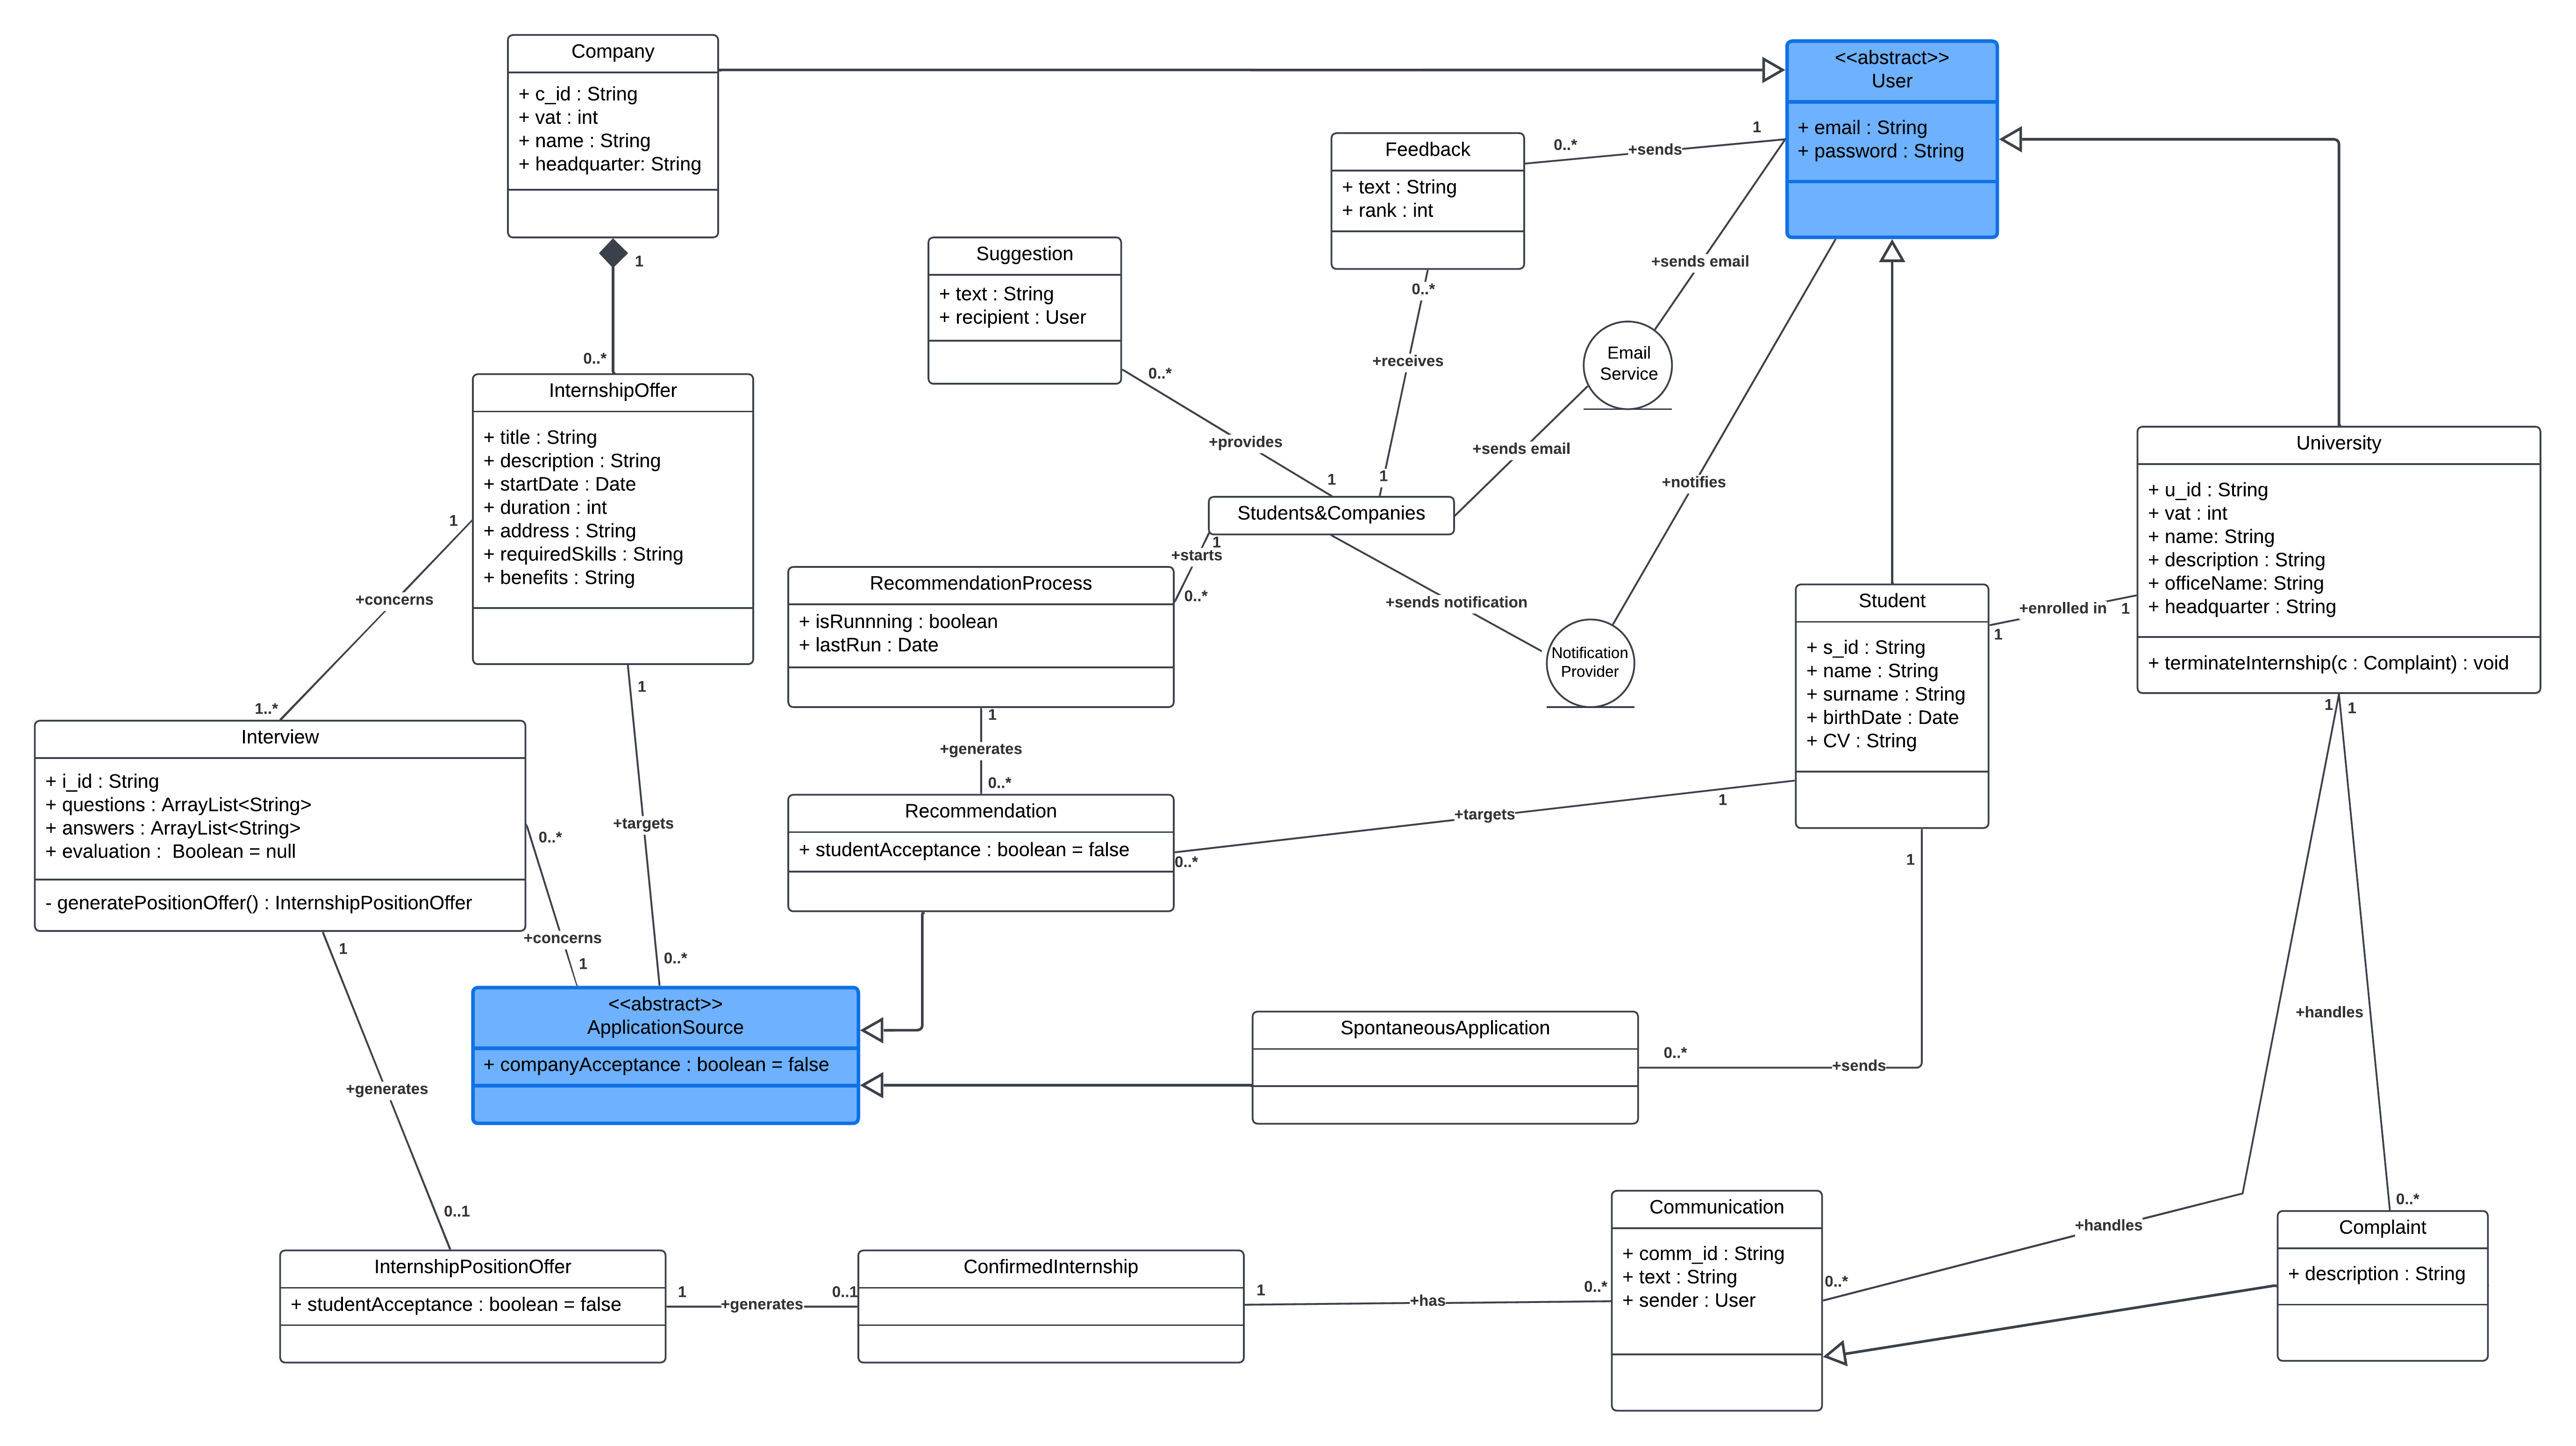
\includegraphics[width=\linewidth]{Latex/Images/ClassDiagram2.1.png}
    \caption{Class Diagram}
    \label{fig:ClassDiagram}
\end{figure}
To clarify the methods signatures:
\begin{itemize}
    \item Interview: \verb|generatePositionOffer(): InternshipPositionOffer| \\generates the \verb|InternshipPositionOffer| if the company wants to provide the student who passed an interview with an Internship Position Offer. 
    \item University: \verb|terminateinternship(c: Complaint): void| \\allows the University to terminate an Internship through a Complaint.
\end{itemize}
Other methods have been omitted for simplicity, as the relations are sufficient to understand the domain. 
\clearpage
\subsubsection{State Charts}
The following section presents a series of state diagrams illustrating the progression of the main phases of the Student\&Company platform. These diagrams include representations of the Recommendation Process and its Spontaneous Application variant, the Interview Process that may result in an Internship Position Offer, and finally, a Selection Process diagram that highlights the relationship between the latter two processes.
These diagrams represent the possible states that the object Interview can be in, without detailing all possible outcomes explicitly. For example, the case of the interview accepted or rejected are represented into a single state, InternshipEnded, without loss of generality.
\newline\newline
\noindent\textbf{\color{titleColor}Recommendation Process}\\
\begin{figure}[ht]
    \centering
    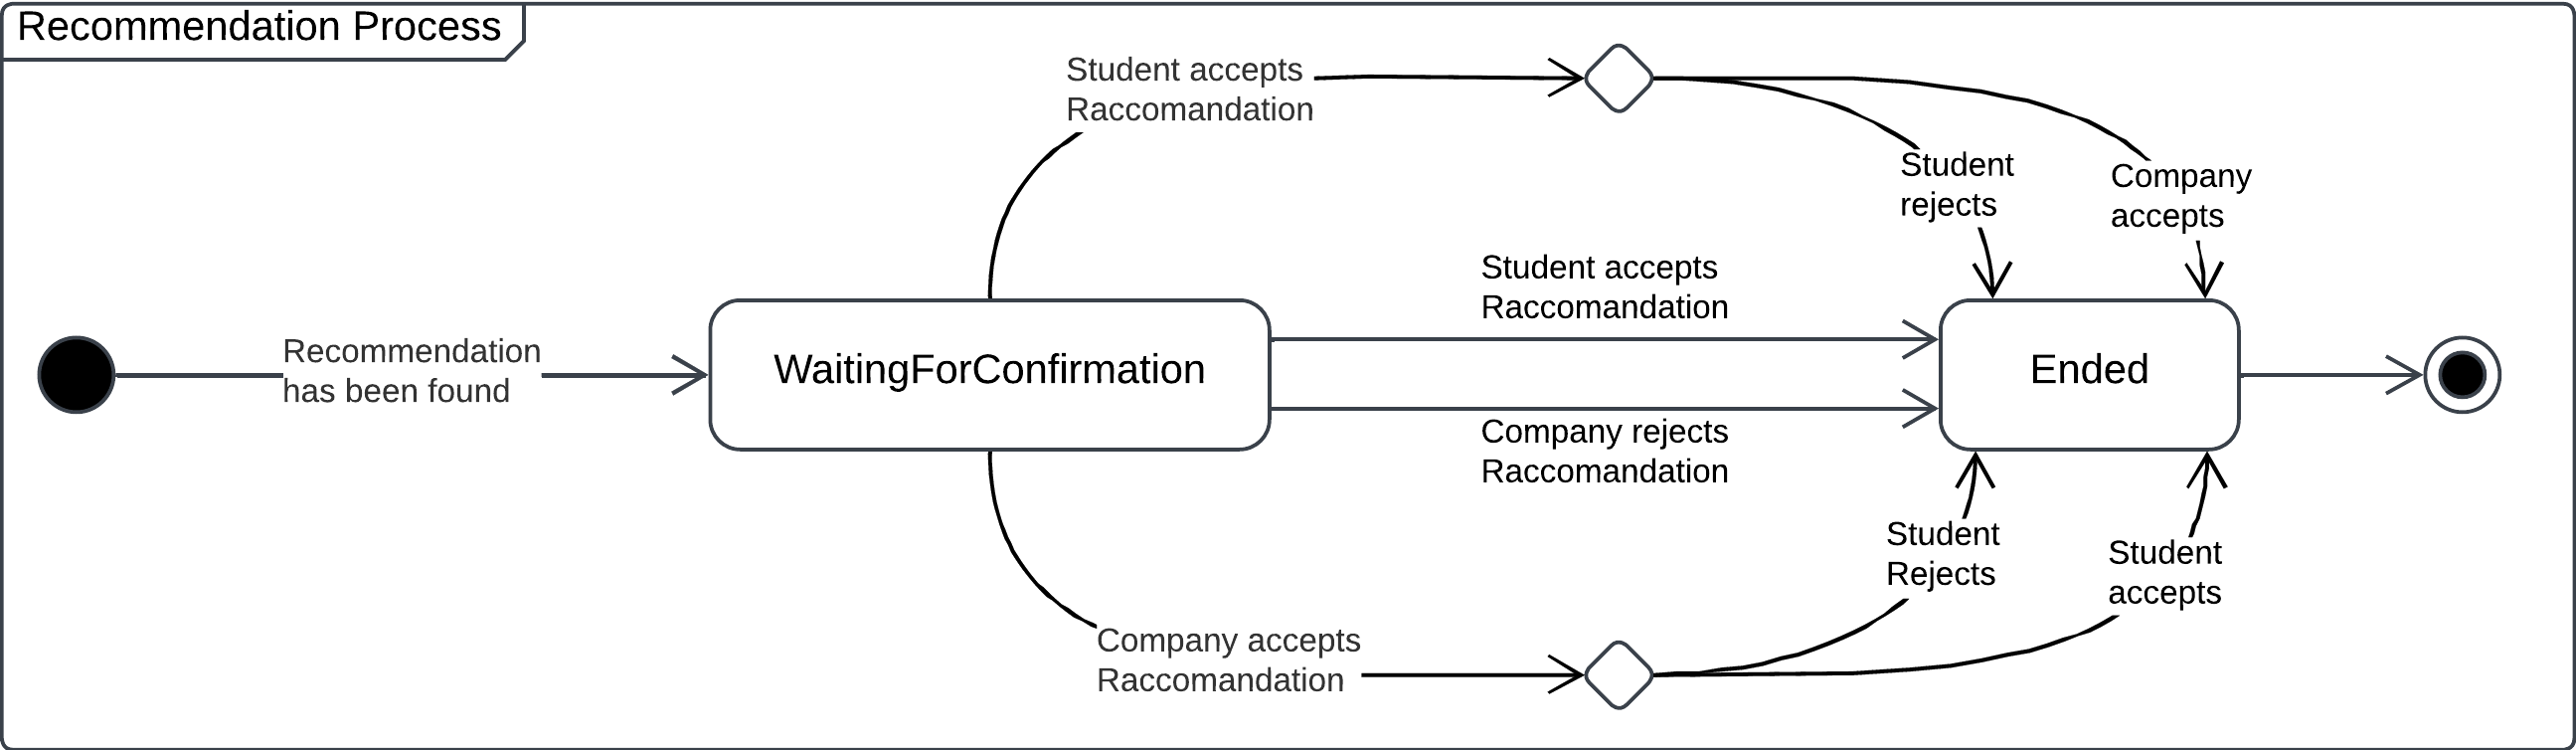
\includegraphics[width=1 \textwidth]{Latex/Images/RecommendationStateChart.png}
    \caption{Recommendation State Chart}
    \label{fig:RecommendationProcess}
\end{figure}
\begin{itemize}
    \item The Recommendation Process is the core of the Student\&Company platform. It is the process that matches Students with Internships based on the Student's CV and the Internship's requirements. It is initiated by the platform when it detects a potential Match. The process then evolves to a "ToBeAccepted" state, where the system waits for the Student and the Company to accept the Match. If one of the two parties rejects the Match, the process is terminated. If both parties accept the Match, an Interview is initiated, and the process is terminated.
\end{itemize}

\noindent\textbf{\color{titleColor}Spontaneous Application Process}\\
\begin{figure}[ht]
    \centering
    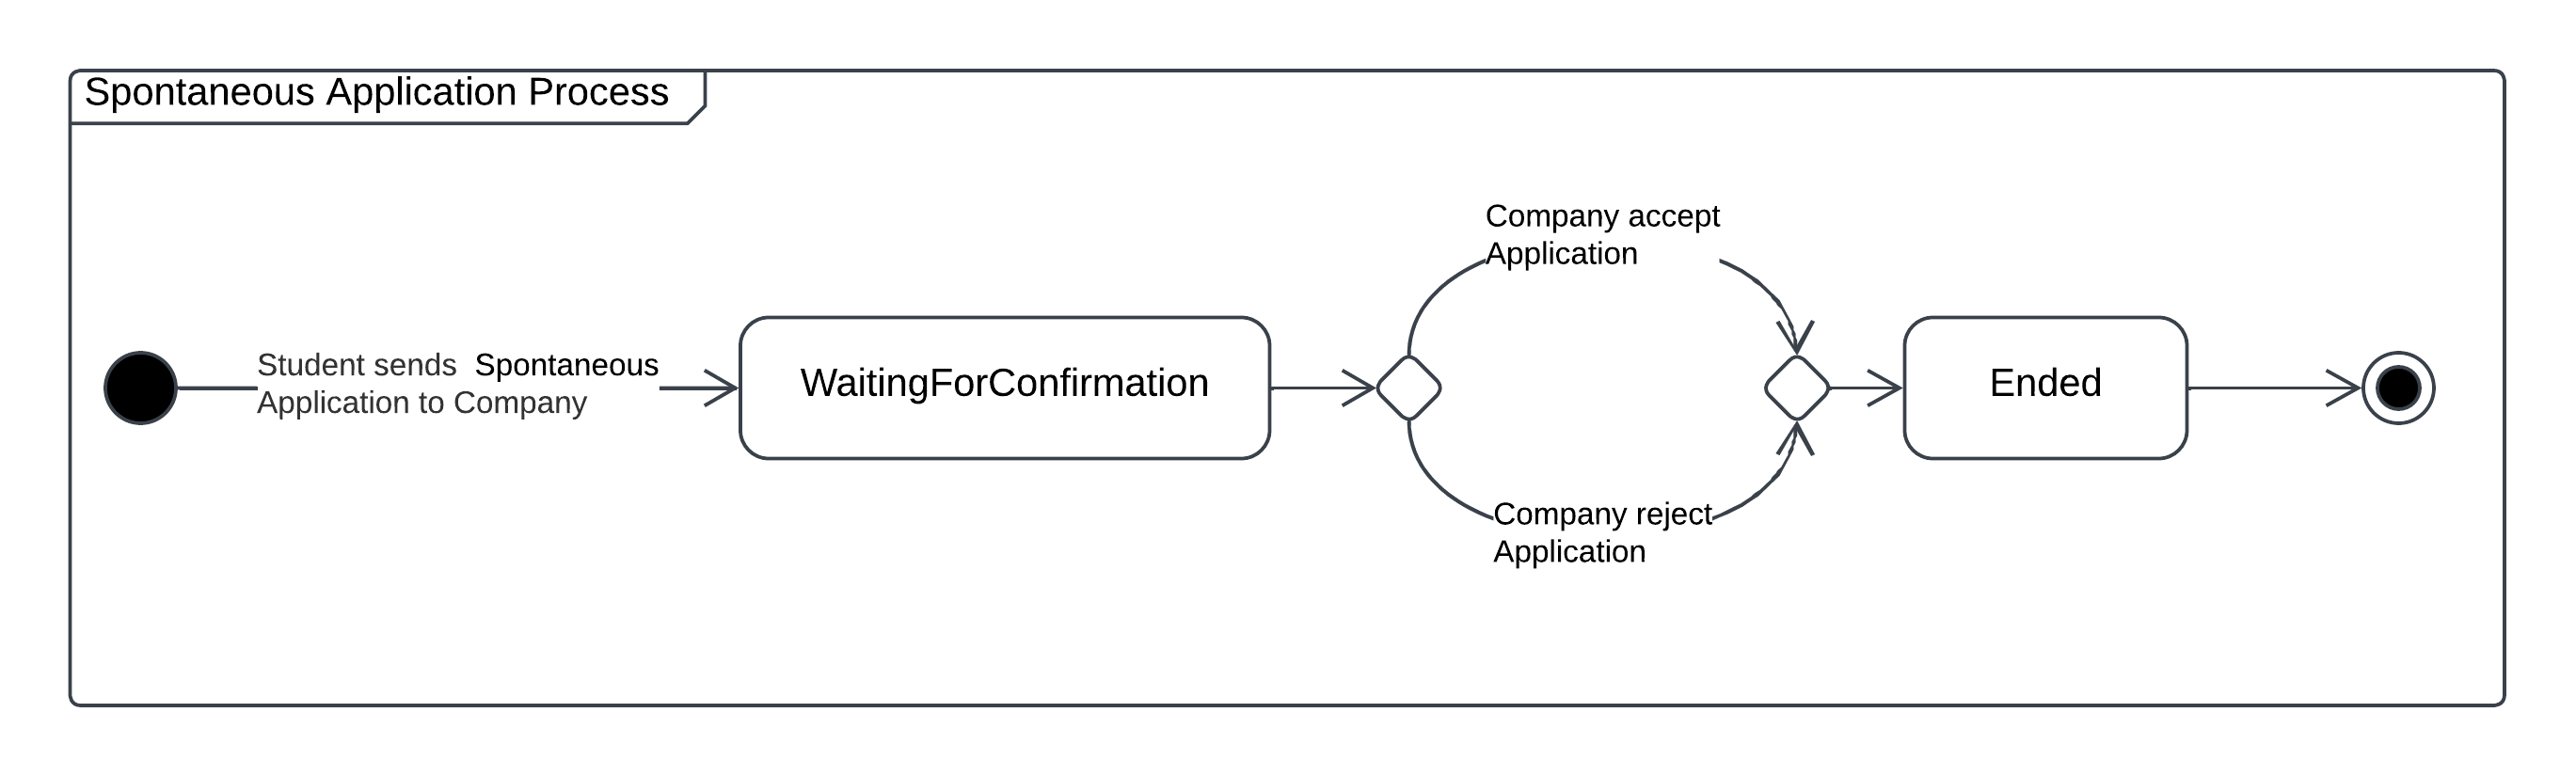
\includegraphics[width=1 \textwidth]{Latex/Images/SpontaneousApplicationStateChart.png}
    \caption{Spontaneous Application State Chart}
    \label{fig:SpontaneousApplication}
\end{figure}
\begin{itemize}
    \item Unlike the Recommendation Process, the Spontaneous Application process is initiated by the Student. When a Student submits a Spontaneous Application for an Internship, the process evolves to a "ToBeAccepted" state, where the system waits for the Company to accept the Application. If the Company rejects the Application, the process is terminated. If the Company accepts the Application, an Interview Process is initiated, and the process is terminated.
\end{itemize} 
\clearpage
\noindent\textbf{\color{titleColor}Interview Process}\\
\begin{figure}[H]
    \centering
    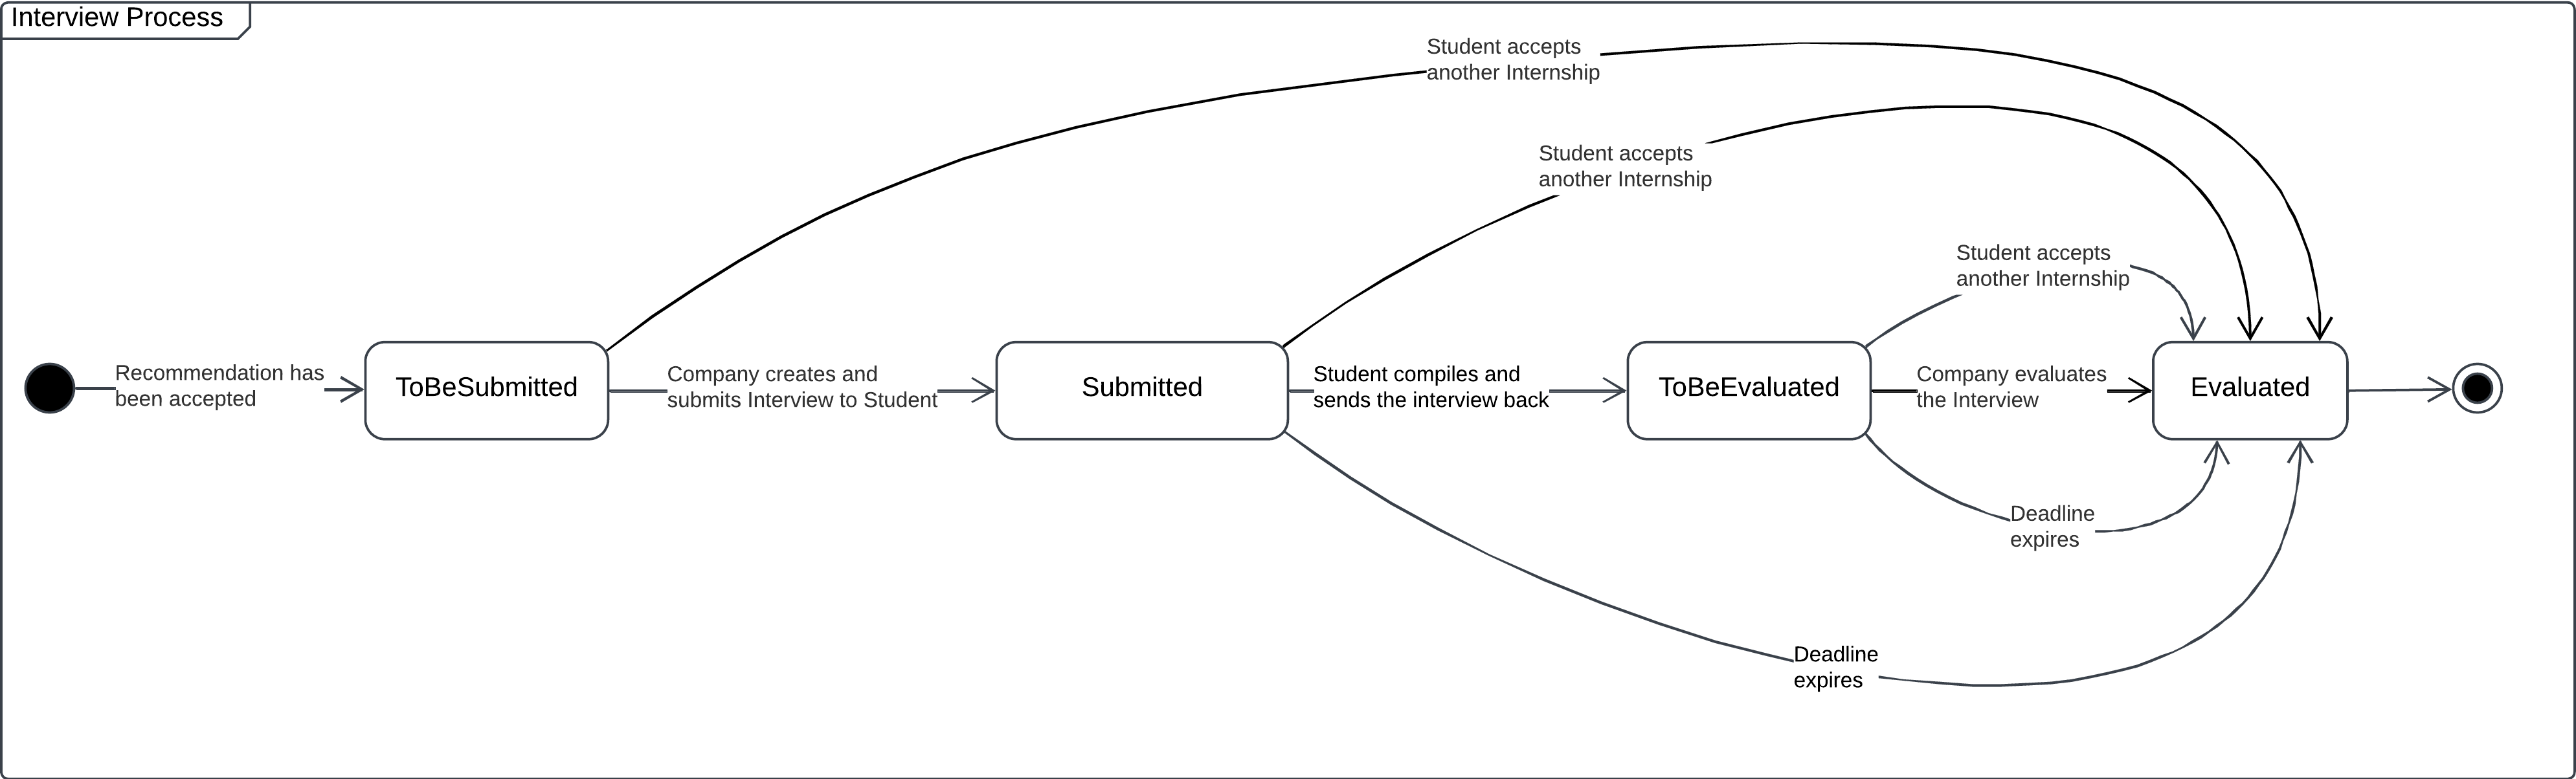
\includegraphics[width=1 \textwidth]{Latex/Images/InterviewProcessStateChart.png}
    \caption{Interview State Chart}
    \label{fig:InterviewProcess}
\end{figure}
\begin{itemize}
    \item The Interview Process is initiated when a Match is accepted by both the Student and the Company, or when the Company accepts a Spontaneous Application. The process starts in the “ToBeSubmitted” state, where the Company is asked to create and submit an Interview. Here, the Company is required to specify a deadline for the Interview. The Interview process evolves into the “Submitted” state once the Company sends the Interview to the Student, who answers the questions and submits the Interview. If the Student fails to submit the answers within the deadline, he will be considered rejected, and the process is progressed to an "Evaluated" state and terminates. Otherwise, after the Interview has been sent back by the student, the process evolves to a “ToBeEvaluated” state. In this state, the Company can manually evaluate the Student's answers and mark the interview as accepted or rejected. In case the Student has been rejected, he will be notified of the outcome, and the process is terminated. Otherwise, if the Student has been accepted, an Internship Position Offer process started and the Interview Process is terminated. If anywhere in the process, the Student accepts another Internship, the process terminates and the Student will be considered rejected.
\end{itemize}

\noindent\textbf{\color{titleColor}Internship Position Offer process}\\
\begin{figure}[H]
    \centering
    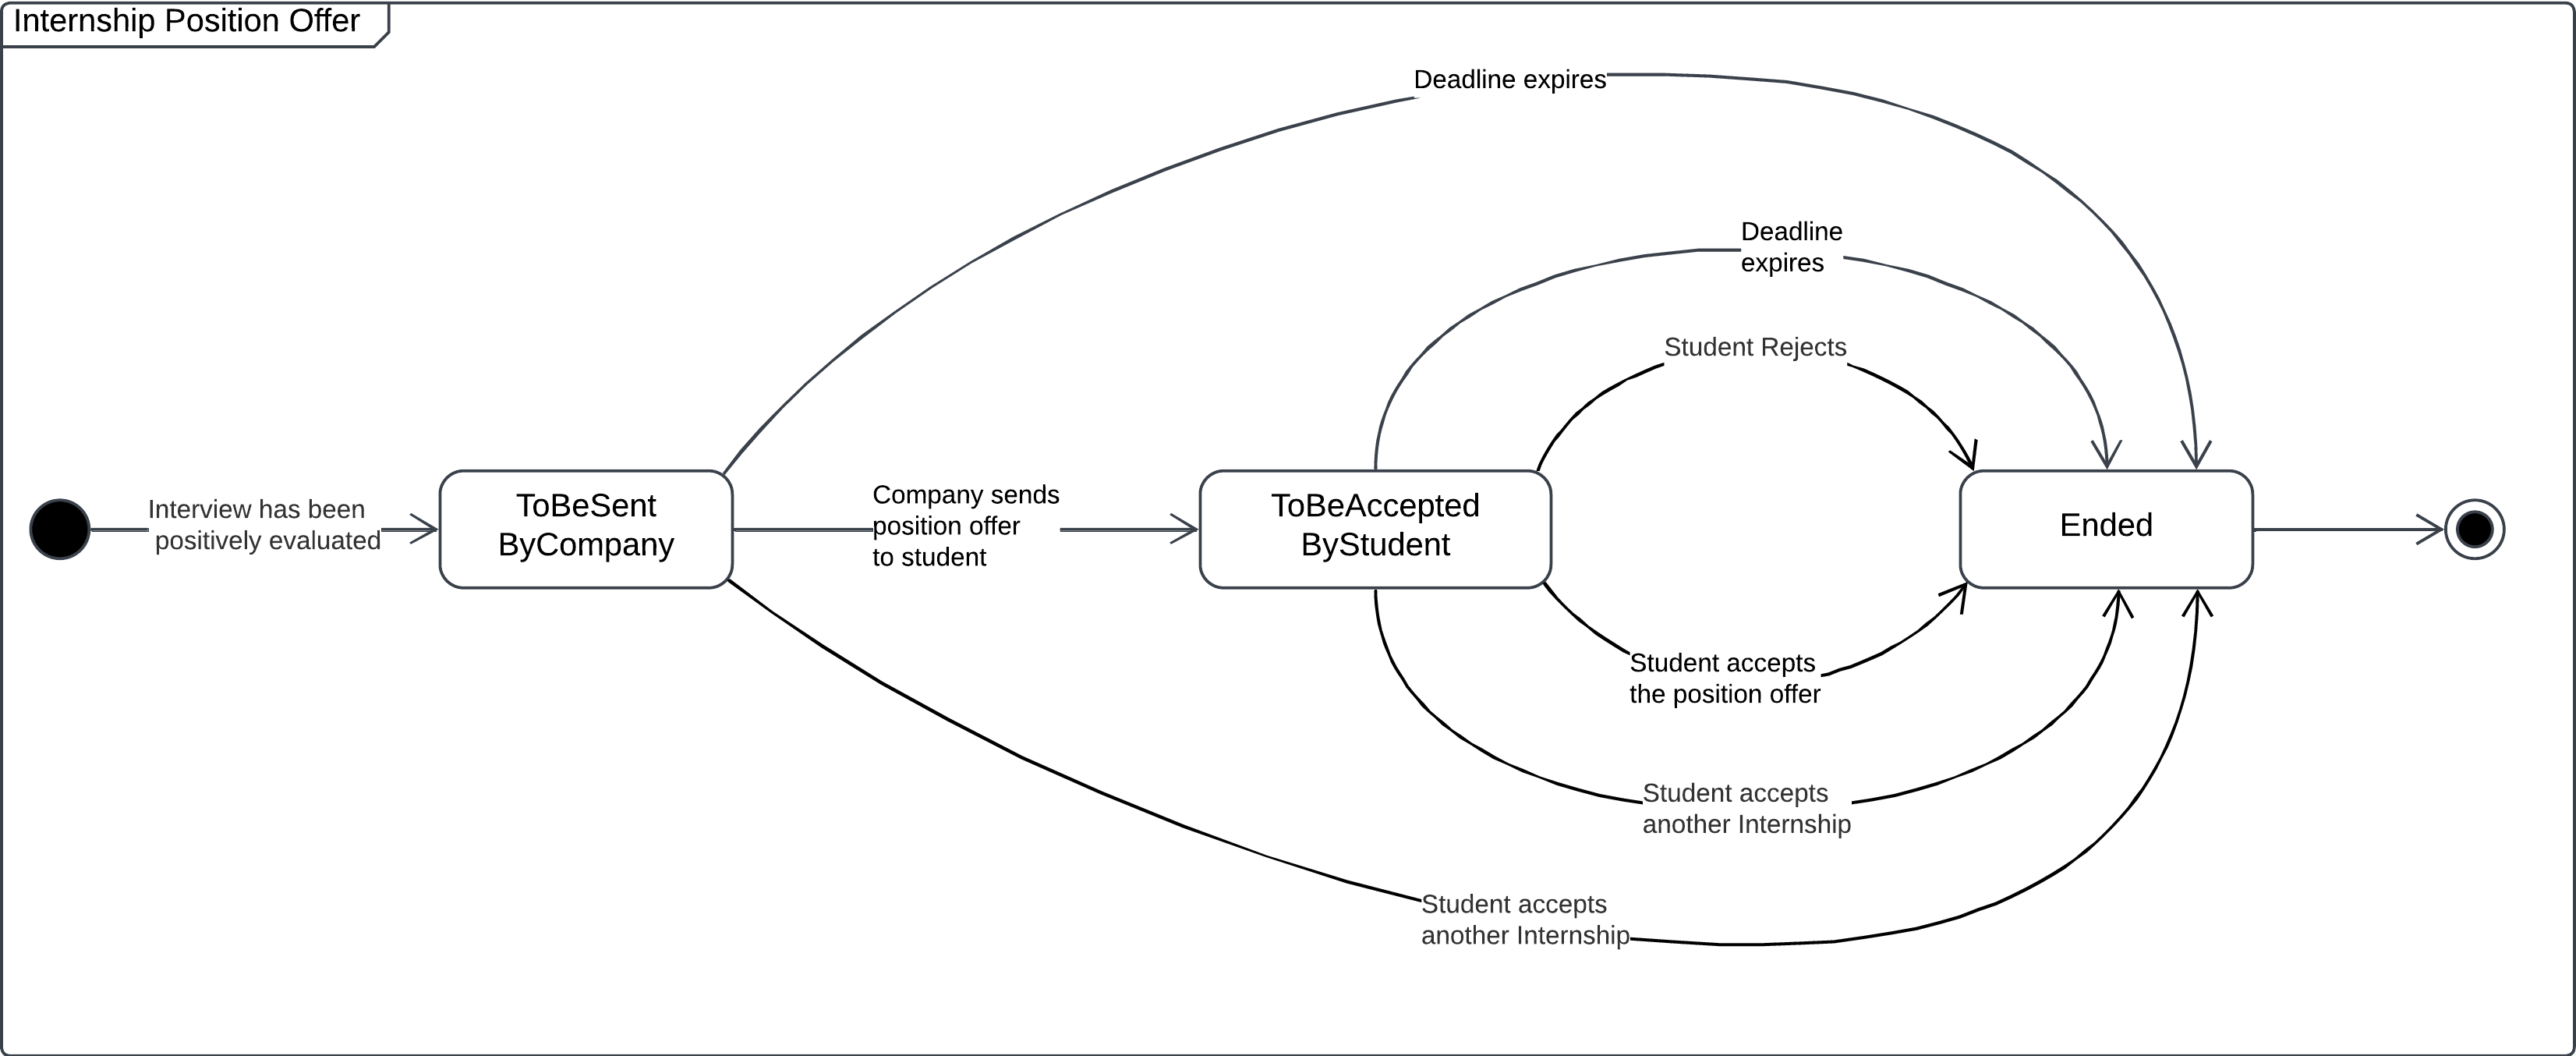
\includegraphics[width=1 \textwidth]{Latex/Images/InternshipPositionOfferStateChart.png}    
    \caption{Internship Position Offer State Chart}
    \label{fig:InternshipPositionOffer}
\end{figure}
\begin{itemize}
    \item The Internship Position Offer process begins when a student successfully completes the Interview Process. Initially, the process enters the “ToBeSentByCompany” state.
    This state allows companies to evaluate and select the most suitable candidates when more students than required have passed the interview.
    If the company rejects the student or the deadline expires, the process concludes, and the student will be considered rejected.
    If the company accepts the student, the process transitions to the “ToBeAcceptedByStudent” state, where the student decides to either accept or reject the offer.
    If the student rejects the offer or lets the deadline expire, the process concludes, and the student will be considered rejected.
    If the student accepts the offer, the process concludes, and all the student’s other ongoing interviews are terminated with the student being marked as rejected in those interviews.
    If anywhere in the process, the Student accepts another Internship, the process is terminated and the Student will be considered rejected.
\end{itemize}

\noindent\textbf{\color{titleColor}Selection Process}\\
\begin{figure}[H]
    \centering
    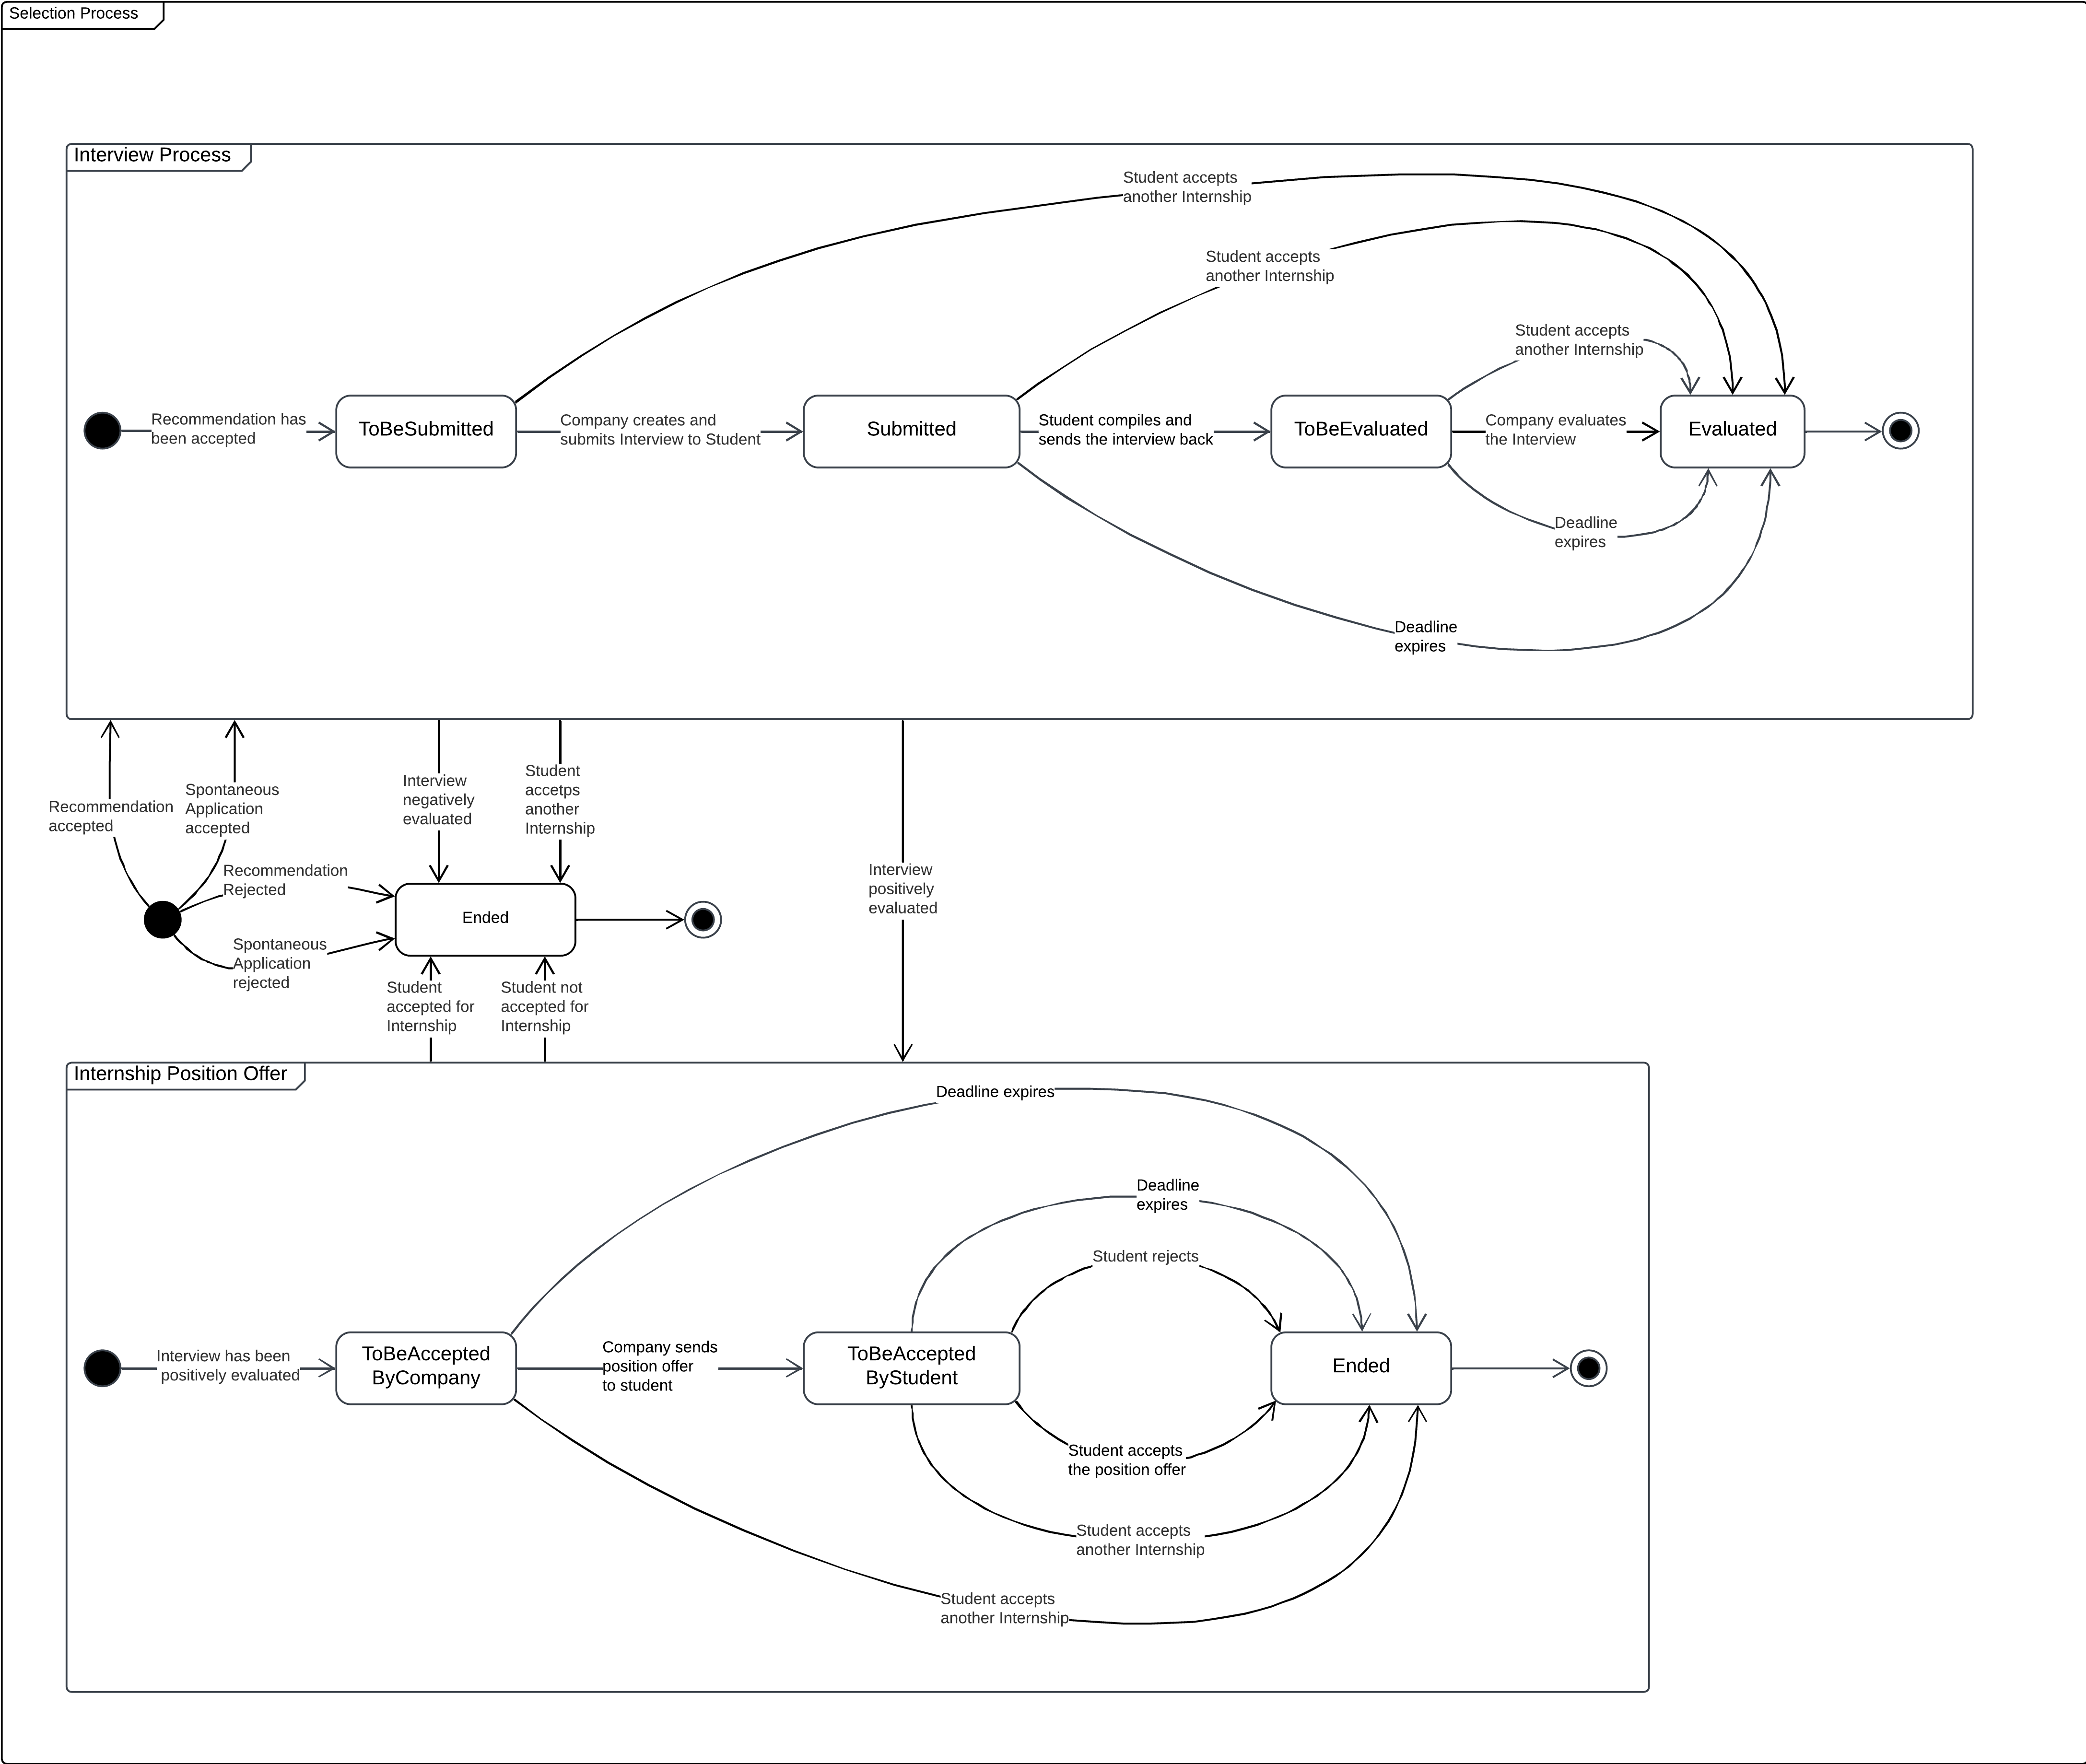
\includegraphics[width=1 \textwidth]{Latex/Images/SelectionProcessStateChart.png}
    \caption{Selection Process State Chart}
    \label{fig:SelectionProcess}
\end{figure}
\begin{itemize}
    \item The Selection Process diagram illustrates the relationship between the Interview Process and the Internship Position Offer Process.
    The Selection Process terminates if the Match is rejected, if the Student is rejected during the Interview Process or the Internship Position Offer Process, or if the Student accepts another Internship.
    If the Student is accepted during the Interview Process, the process transitions to the Internship Position Offer Process.
    If the Student accepts the Internship Position Offer, the process also concludes.
\end{itemize}
\clearpage
\subsection{Product Functions}
This section outlines the essential functionalities and detailed requirements of the platform, structured to support the key objectives defined in the scope of the product.
\begin{enumerate}
    \item \textbf{\color{titleColor}User Management}: The platform allows Students, Companies, and Universities to register and log in. It also provides Students with the ability to upload and modify their CVs, and Companies with the ability to view and manage their Internships.
    \item \textbf{\color{titleColor}Internship Creation and Management}: Companies can create, publish, and manage Internship offers on the platform. They define details such as job description, requirements, deadlines, and benefits. Companies also have the ability to terminate Internship offers when they are no longer available.
    \item \textbf{\color{titleColor}Student Application Process}: Students can browse available Internships and apply to Internships either through automatic matching or by submitting Spontaneous Applications. They can also track the status of their Applications throughout the process.
    \item \textbf{\color{titleColor}Automated Recommendations}: The platform matches Students with suitable Internships based on their CVs and the specific requirements set by Companies. Once a match is found, both Students and Companies are notified, and they can accept or decline the Recommendation.
    \item \textbf{\color{titleColor}Interview Management}: Companies can create and assign Interviews to Students, which include closed and open questions to assess their suitability for an Internship. Both Students and Companies can track the Interview progress, and Companies can evaluate Student responses. Companies can also select among students who have passed the interview those to whom they will propose an Internship Position Offer.
    \item \textbf{\color{titleColor}Feedback and Suggestions for Improvement}: The platform collects Feedback from Students and Companies to improve the Recommendation Process. It also provides Suggestions to Students on how to enhance their CVs and to Companies on how to improve their Internship descriptions.
    \item \textbf{\color{titleColor}Complaint Management}: Students and Companies can publish Complaints about Ongoing Internships, which are then handled by Universities. Universities can monitor Complaints and interrupt Ongoing Internships if necessary.
    \item \textbf{\color{titleColor}Notification System}: Notifications are sent to Students, Companies, and Universities when relevant events occur, such as new Internships, matched Recommendations, Interview assignments,  Internship Position Offers, Sign-up confirmation, Complains or Communications.
\end{enumerate}

\subsubsection{Requirements}
\begin{enumerate}[label={\color{titleColor}[R\arabic*]}]
    % Login
    \item The platform shall allow any unregistered students to register by providing personal information and selecting their University.
    \item The platform shall allow any companies to register by providing company information.
    \item The platform shall allow any universities to register by providing university information.
    \item The platform shall allow Users to log in using their email and password.
    \item The platform shall send notifications to Users when relevant events occur.
    
    % Application advertisement and Applications
    \item The platform shall allow Companies to create and publish Internship offers specifying details.
    \item The platform shall allow Companies to terminate their Internship offers at their own discretion.
    \item The platform shall provide Students with Matches automatically obtained by the Recommendation Process.
    \item The platform shall allow Students to view and navigate all available Internships.
    \item The platform shall enable Students to submit Spontaneous Applications to Internships they choose.
    \item The platform shall allow Students to submit their CV.
    \item The platform shall allow Students to modify their CV.
    \item The platform shall allow Students to monitor the status of their Spontaneous Applications.
    \item The platform shall allow Students to monitor the status of their Recommendation.
    
    % Recommendation system
    \item The platform shall display to Students all the Internships found by the Recommendation Process.
    \item The platform shall display to Companies all the CVs of Matched Students obtained by the Recommendation Process.
    \item The platform shall allow Students and Companies to accept a Recommendation.
    \item The platform shall allow Companies to accept a Spontaneous Application.
    \item The platform shall start a Selection Process only if both the Company and the Student have accepted the Recommendation.
    \item The platform shall start a Selection Process only if the Company has accepted the Spontaneous Application.
    
    % Selection and Interview Management
    \item The platform shall allow Companies to create Interviews.
    \item The platform shall allow Companies to submit Interviews to Students they have initiated a Selection Process with.
    \item The platform shall allow Students to answer Interview questions and submit them.
    \item The platform shall allow Companies to manually evaluate Interview submissions.
    \item The platform shall allow Students and Companies to monitor the status of their Interviews.
    \item The platform shall enable Companies to complete the Interview process by submitting the final outcome to each candidate.

    %Internship Position Offer
    \item The platform shall enable Companies to send an Internship Position Offer to a Student only if he previously passed the relative Interview.
    \item The platform shall enable Students to accept or reject an Internship Position Offer sent by a Company only if he previously passed the relative Interview.
    
    % Feedback and Suggestions for Improvements
    \item The platform shall collect Feedback from both Students and Companies regarding the Recommendation Process.
    \item The platform shall provide Suggestions to Students on improving their CVs.
    \item The platform shall provide Suggestions to Companies on improving Internship descriptions.
    
    % Universities Oversight and Complaint Management
    \item The platform shall allow registered Universities to access and monitor Internship Communications related to their Students.
    \item The platform shall provide a dedicated space for Students and Companies to exchange Communications about the current status of an Ongoing Internship.
    \item The platform shall allow registered Universities to handle Complaints and to interrupt an Internship at their own discretion.
\end{enumerate}


\subsection{User Characteristics}
Student\&Company is designed to be used by three main types of Users: Students, Companies, and Universities. Each User has a specific role and can perform different actions on the platform as described below:
\begin{itemize}
  \item \textbf{Students}: \\
    Students are individuals currently enrolled in a University (which must be registered on the Platform) who are looking for Internship opportunities to enhance their education and their curriculum. \\
    They can register on the platform, upload their CVs, and apply for Internships either through the Recommendation Process or by submitting a Spontaneous Applications to an Interview Offer to which they are particularly interested. Students can also monitor the status of their Applications, Interviews, and Internship Position Offers through a dedicated section on the platform and, if necessary, can report problems encountered during an Ongoing Internship to their University by creating a Complaint.\\
    The platform also provides Students with Suggestions on how to improve their CVs and matching probability based on a grammar and lexical analysis and a direct comparison of the Student's CV with others similar candidate. The Student can also improve the platform by providing Feedback on the Recommendation Process once a Confirmed Match is found.
  \item \textbf{Companies}:\\
    Companies are entities that are looking for interns to train and educate in their field of expertise. Each company account is created by a representative of the Company, usually a Human Resource employee or a manager that is in charge of the internship program. \\
    Companies can register on the platform and create, publish, manage and delete different Internship Offers at the same time. They can also view and manage the CVs of Students that have been matched or have sent a Spontaneous Application to such offers, and create and submit Interviews to evaluate them. If a Student passes the Interview, the Company can send an Internship Position Offer to him while monitoring other Interviews and Internship Position Offers and, moreover, each Company can report problems encountered during an Ongoing Internship by creating Complaints.\\
    The platform also provides Companies with Suggestions on how to improve their Internship descriptions and matching probability based on a grammar and lexical analysis and a direct comparison of the Company's Internship Offer with other similar companies. They can also help improve the platform by providing Feedback on the Recommendation Process once a Confirmed Match is found.
  \item \textbf{Universities}:\\
    Universities are institutions that are looking to provide their Students with Internship opportunities to enhance their education and curriculum. Each university account is created by a representative of the University, usually a carrier advisor or a professor that is in charge of the internship program.\\
    Universities can register on the platform and monitor their Students by receiving Communication both from Student and Companies. Such Communication can be about the acceptance of an Internship Position Offer by a Student or some problem encountered during an Ongoing Internship reported by a party trough a Complaint. \\
    The University can handle such Complaints and, eventually, interrupt an Ongoing Internship if no solution to the problem is found to prevent further issues.
\end{itemize}
While Student\&Company is not specifically designed to accommodate users with special needs, the platform implements several basic accessibility features to improve usability for all users. These include different display modes such as dark mode, screen-reader compatible layouts and easily readable fonts.
The web interface try to follow WCAG 2.1 Level A guidelines for basic accessibility compliance. However, users requiring specialized assistive technologies may need to rely on their own tools and software to interact with the platform optimally.\\

\subsection{Assumptions, dependencies, and constraints}

\subsubsection{Domain Assumption}
This section outlines the basic assumptions about the environment and behavior of entities that interact with the system. These assumptions simplify the design and implementation by defining expectations about Students, Companies, Universities, and the platform, ensuring the system operates effectively within its intended context.
\begin{enumerate}[label={\color{titleColor}[D\arabic*]}]
    \item Students and Companies provide the Platform with correct and truthful information.
    \item Companies remove published Internships if they are no longer available.
    \item The Email Provider and Notification Manager services are reliable, and the Users visualize every notification
    \item Students, Companies, and Universities have a working internet connection.
    \item Universities interrupt an Ongoing Internship only if no solution is found to the Complaints.
\end{enumerate}

\subsubsection{Dependencies}
The platform depends on only two external actors: the Notification Provider and the Email Service.
The former is responsible for correctly handling notifications to ensure they are sent to Users. 
The latter is responsible for sending emails, mainly for users' email verification. For more details, see section \ref{subsec:SWInteface} 
    %------------------------------------------------------------------------------------------------------------------------------------------------
    \clearpage
    \section{Specific Requirements}
    \label{sect:requirements}
    \subsection{External Interface Requirements}
This chapter provides a detailed description of the system's external interfaces such as the User, Hardware, Software, and Communication interfaces. 
\subsubsection{User Interfaces}
The user interface will be designed to improve intuitiveness and simplicity. The platform root page is the Home Page from which every non-registered user can find information about S\&C such as the latest news. The Home page is linked to other pages, such as the Dashboard, Contacts, and About page, using an app bar. 
In the Contacts page, the user can find useful links to get in touch with S\&C.\\
\begin{figure}[H]
    \centering
    
\includegraphics[width=\textwidth]{Latex/Images/UI/v1/HomePage.png}
    \caption{UI Home Page: as an example, UI cards containing some user scenarios described in the \ref{subsec: user scenarios}  are shown}
    \label{fig:homepage}
\end{figure}
\begin{figure}[H]
    \centering
    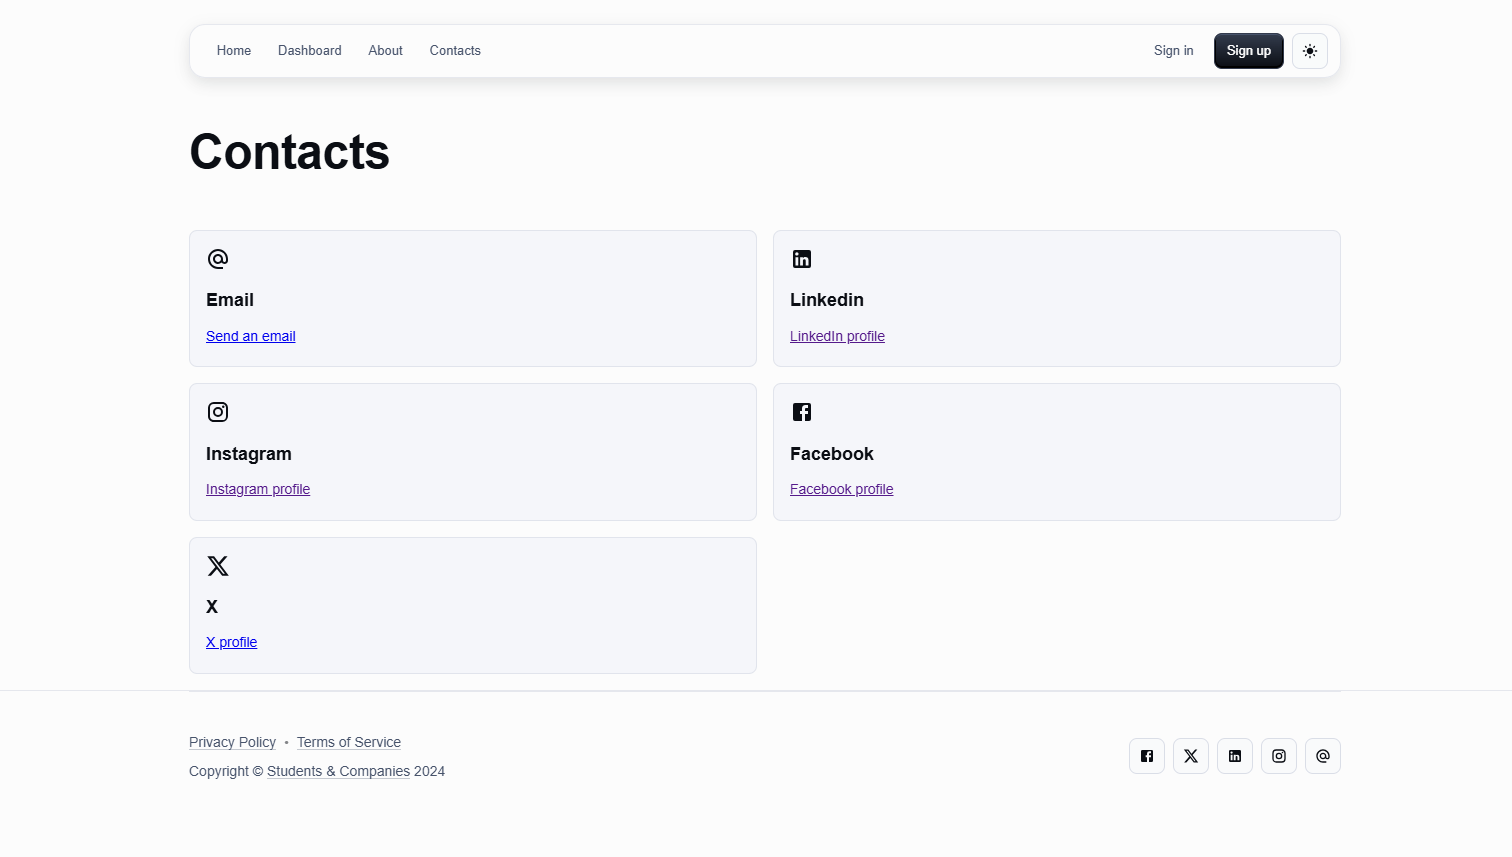
\includegraphics[width=\textwidth]{Latex/Images/UI/v2/Contacts.png}
    \caption{UI Contacts Page}
    \label{fig:contactpage}
\end{figure}
\noindent Thanks to the app bar link buttons, users can also reach the Sign-Up and Sign-in pages. The Sign-Up page allows for different types of sign-up according to the new user type. This allows the user to provide the platform with the correct information.
\begin{figure}[H]
    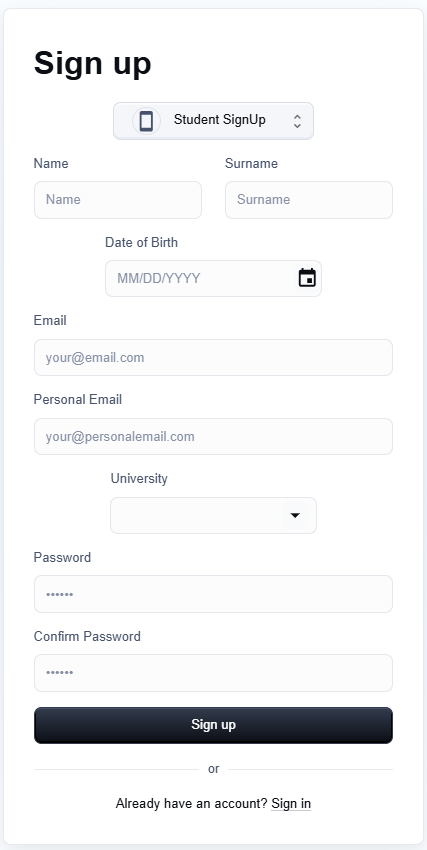
\includegraphics[width=0.33\textwidth]{Latex/Images/UI/v2/SignUp Student.png}
    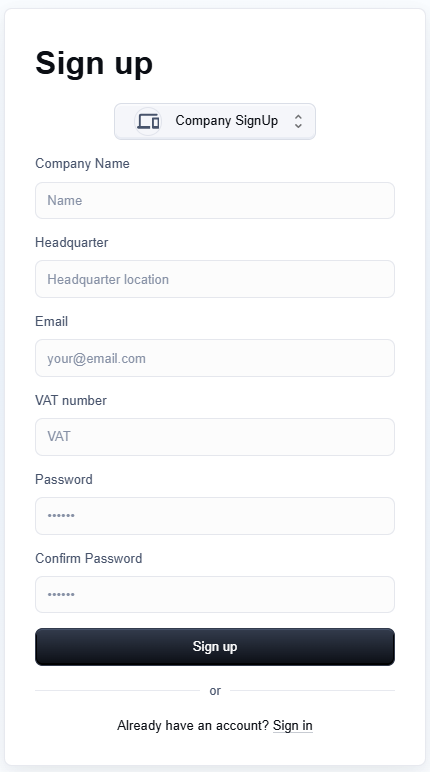
\includegraphics[width=0.33\textwidth]{Latex/Images/UI/v2/SignUp Company.png}
    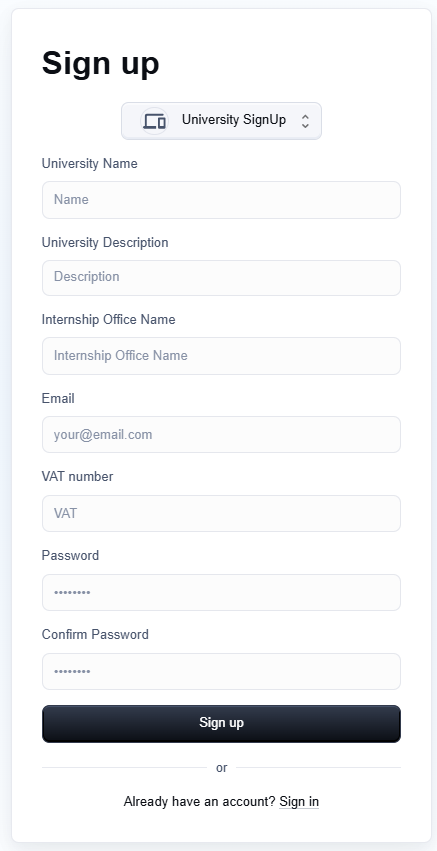
\includegraphics[width=0.33\textwidth]{Latex/Images/UI/v2/SignUp University.png}
    \caption{UI Sign-Up Page}
    \label{fig:signuppage}
\end{figure}
To be able to log into the platform, the user shall provide his email and password. 
\begin{figure}[H]
    \centering
    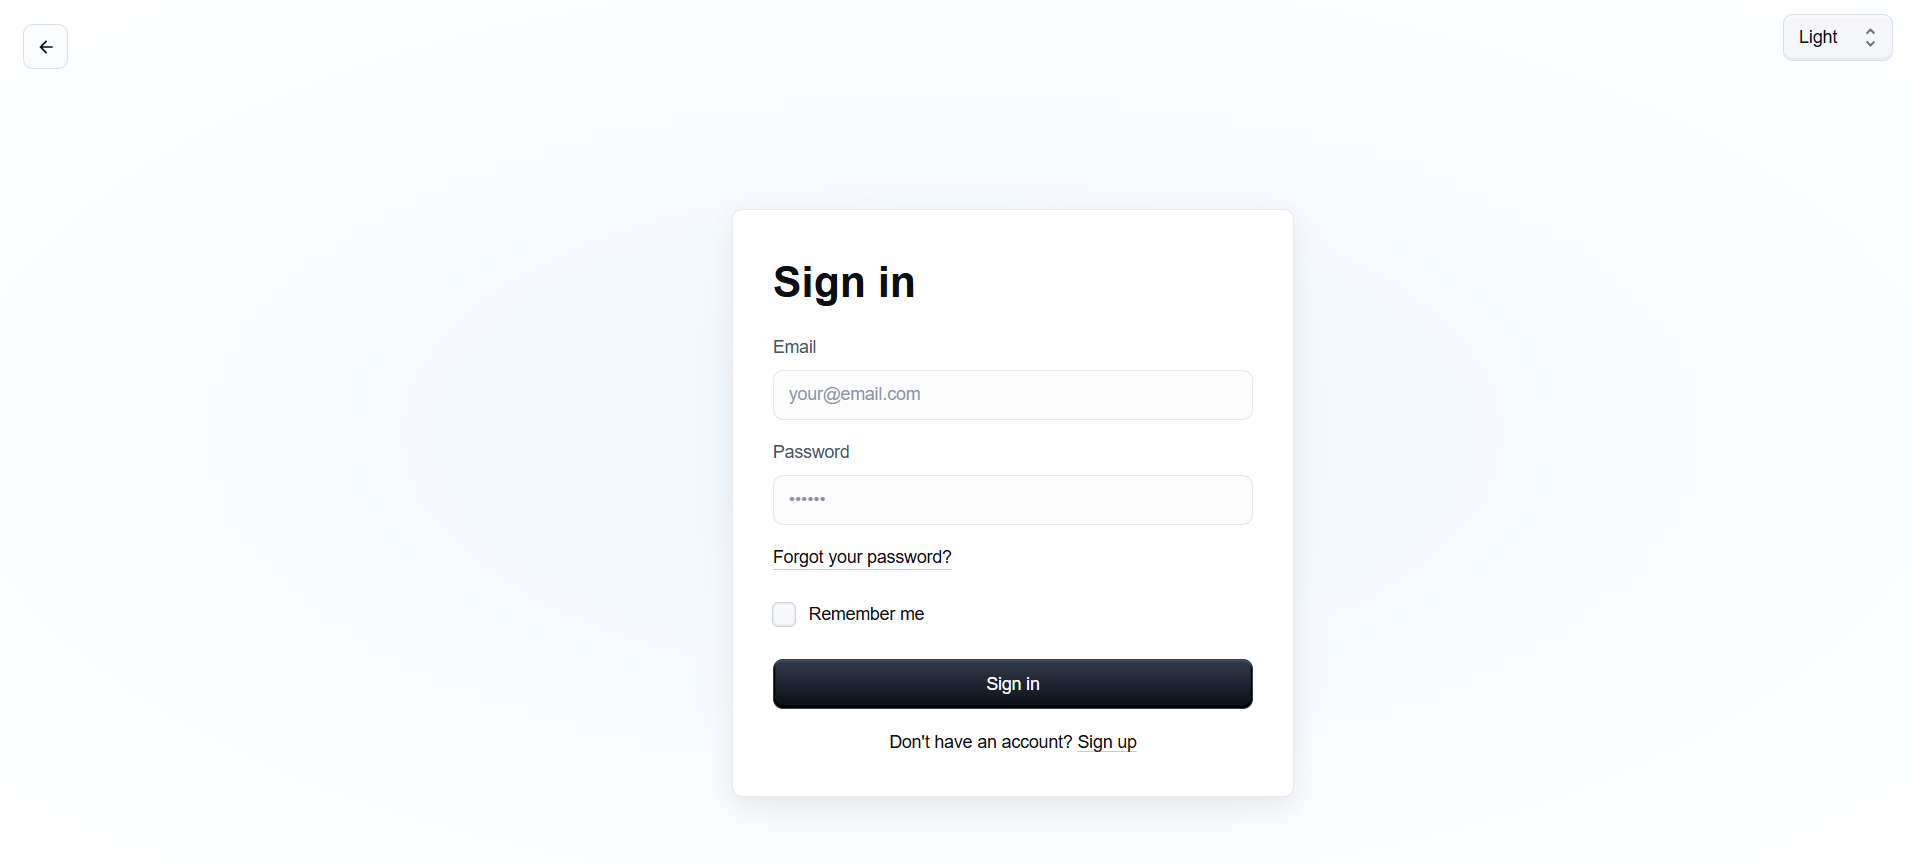
\includegraphics[width=\textwidth]{Latex/Images/UI/v2/SignInPage.png}
    \caption{UI Sign-In Page}
    \label{fig:signinpage}
\end{figure}
\noindent The Dashboard page will be the central hub for logged-in users. From the left-hand panel of the dashboard, all the pages associated with the core functionalities of the platform are reachable. Therefore, this page is provided after a successful log-in. The side panel contains different elements according to the user needs.
\begin{figure}[H]
    \centering
    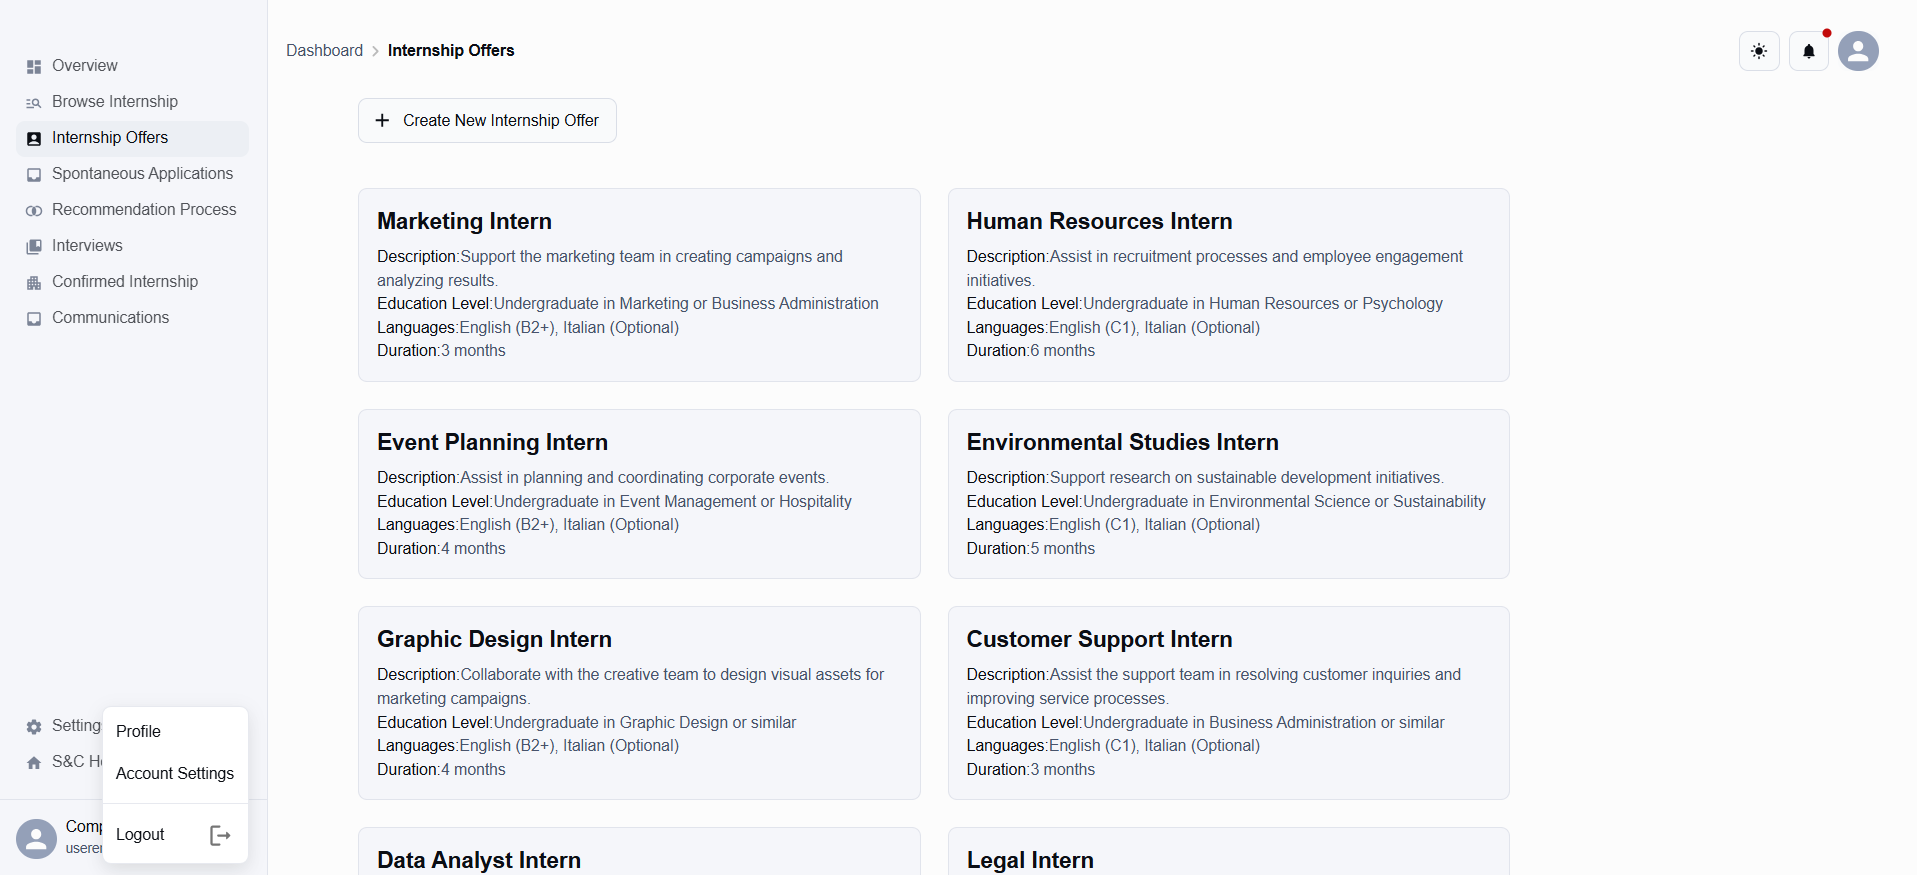
\includegraphics[width=\textwidth]{Latex/Images/UI/v2/Company-Dashboard.png}
    \caption{UI Company Dashboard Page}
    \label{fig:companyDashboard}
\end{figure}
\begin{figure}[H]
    \centering
    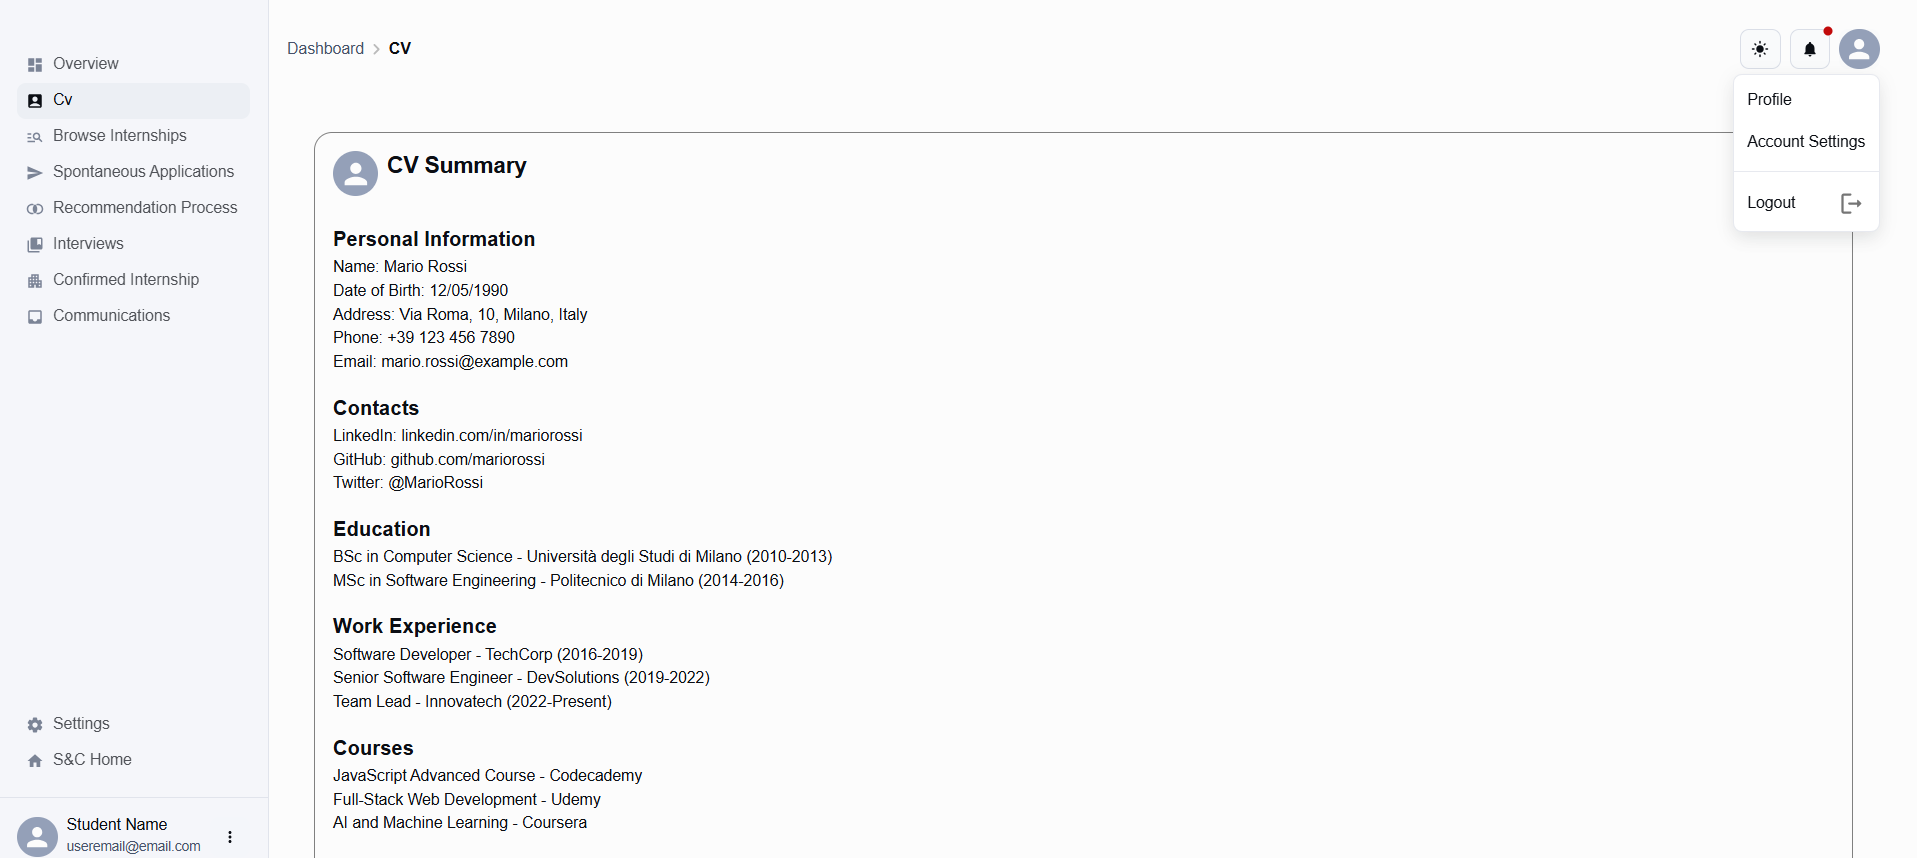
\includegraphics[width=\textwidth]{Latex/Images/UI/v2/Student-Dashboard.png}
    \caption{UI Students Dashboard Page}
    \label{fig:studentDashboard}
\end{figure}
\begin{figure}[H]
    \centering
    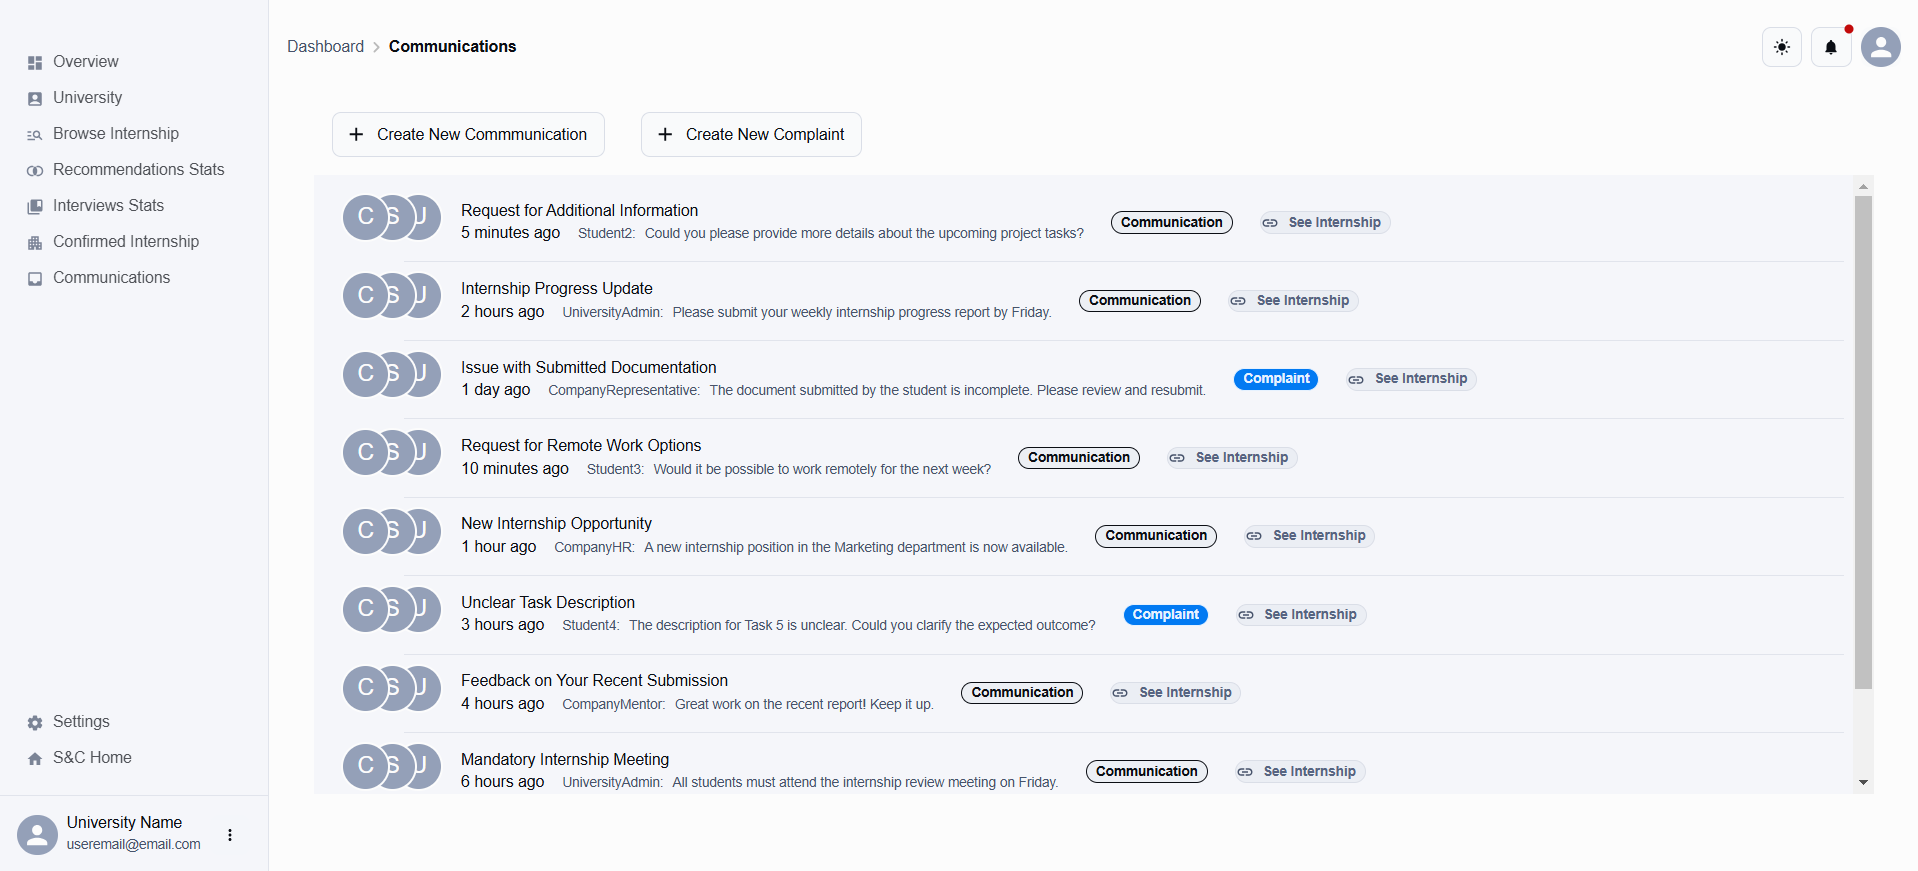
\includegraphics[width=\textwidth]{Latex/Images/UI/v2/Uni-Dashboard.png}
    \caption{UI University Dashboard Page}
    \label{fig:universityDashboard}
\end{figure}

\subsubsection{Hardware Interfaces}
The platform is a web application that can be accessed from any device with a web browser and an internet connection like a PC, a tablet, or a smartphone. No specific hardware requirements are needed to interact with the Student\&Company platform.
\subsubsection{Software Interfaces}
\label{subsec:SWInteface}
An Email Provider, through its interface, is used by the Platform to send a confirmation email to Users upon registration. \\
A notification manager is used to send notification to Users when relevant events occur. Using notifications instead of email allows the platform to provide a more immediate and interactive experience to the Users without generating spam that can be seen as annoying by the Users.\\
At this stage of development, no other external software interfaces are required.
\subsubsection{Communication Interfaces}
The platform uses standard internet communication protocols to interact with Users and the backend server. At this stage of development other specific communication interfaces are not defined yet.

\subsection{Functional Requirements}
This chapter provides a comprehensive overview of the system's use cases, detailing the various interactions between Users and the system.
Use Case Diagrams, detailed Use Case Descriptions, Sequence Diagrams and Requirement Mapping are provided for each use case.
\subsubsection{Use Case Diagrams}
\begin{figure}[H]
    \centering
    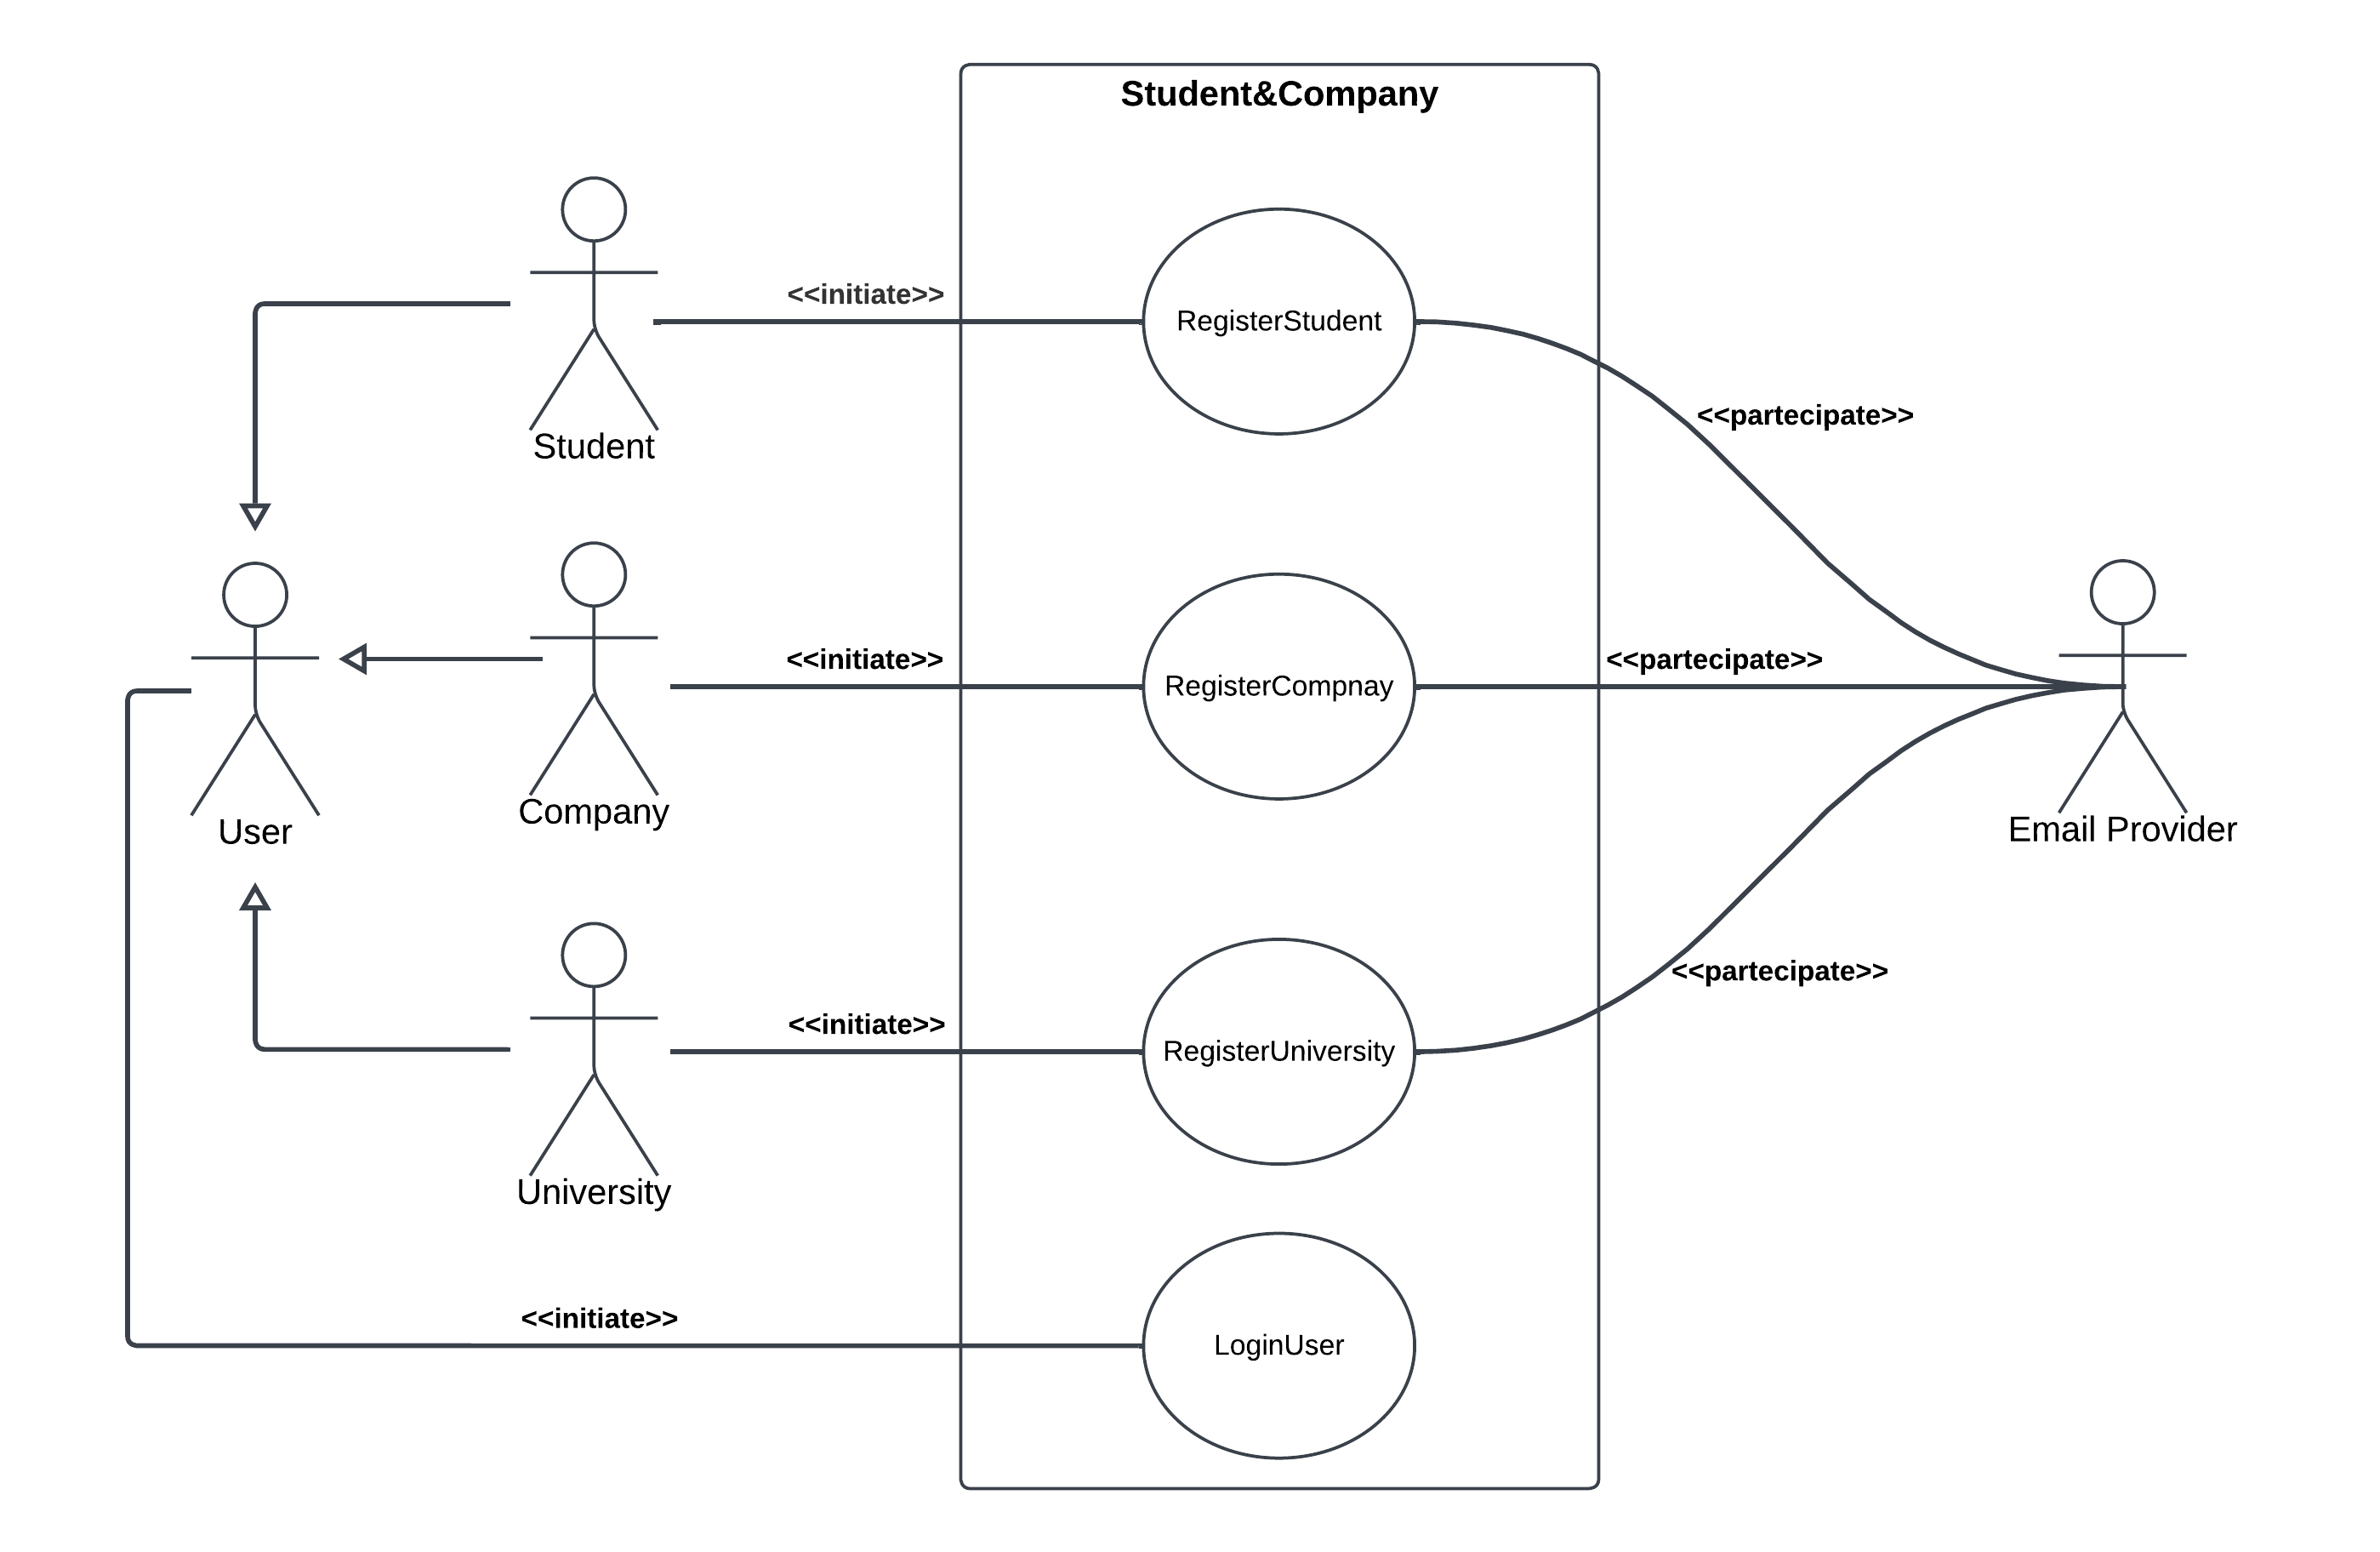
\includegraphics[width=1 \textwidth]{Latex/Images/RASD/UseCases/UserRegistrationUseCase.png}
    \caption{User Registration Use Case Diagram}
    \label{fig:UserRegistrationUseCaseDiagram}
\end{figure}
This diagram illustrates the User Registration and Login process, for all Users. It shows how the different use case for the registration, based on the User type, and how the login process is generic and common for all Users
\clearpage.
\begin{figure}[H]
    \centering
    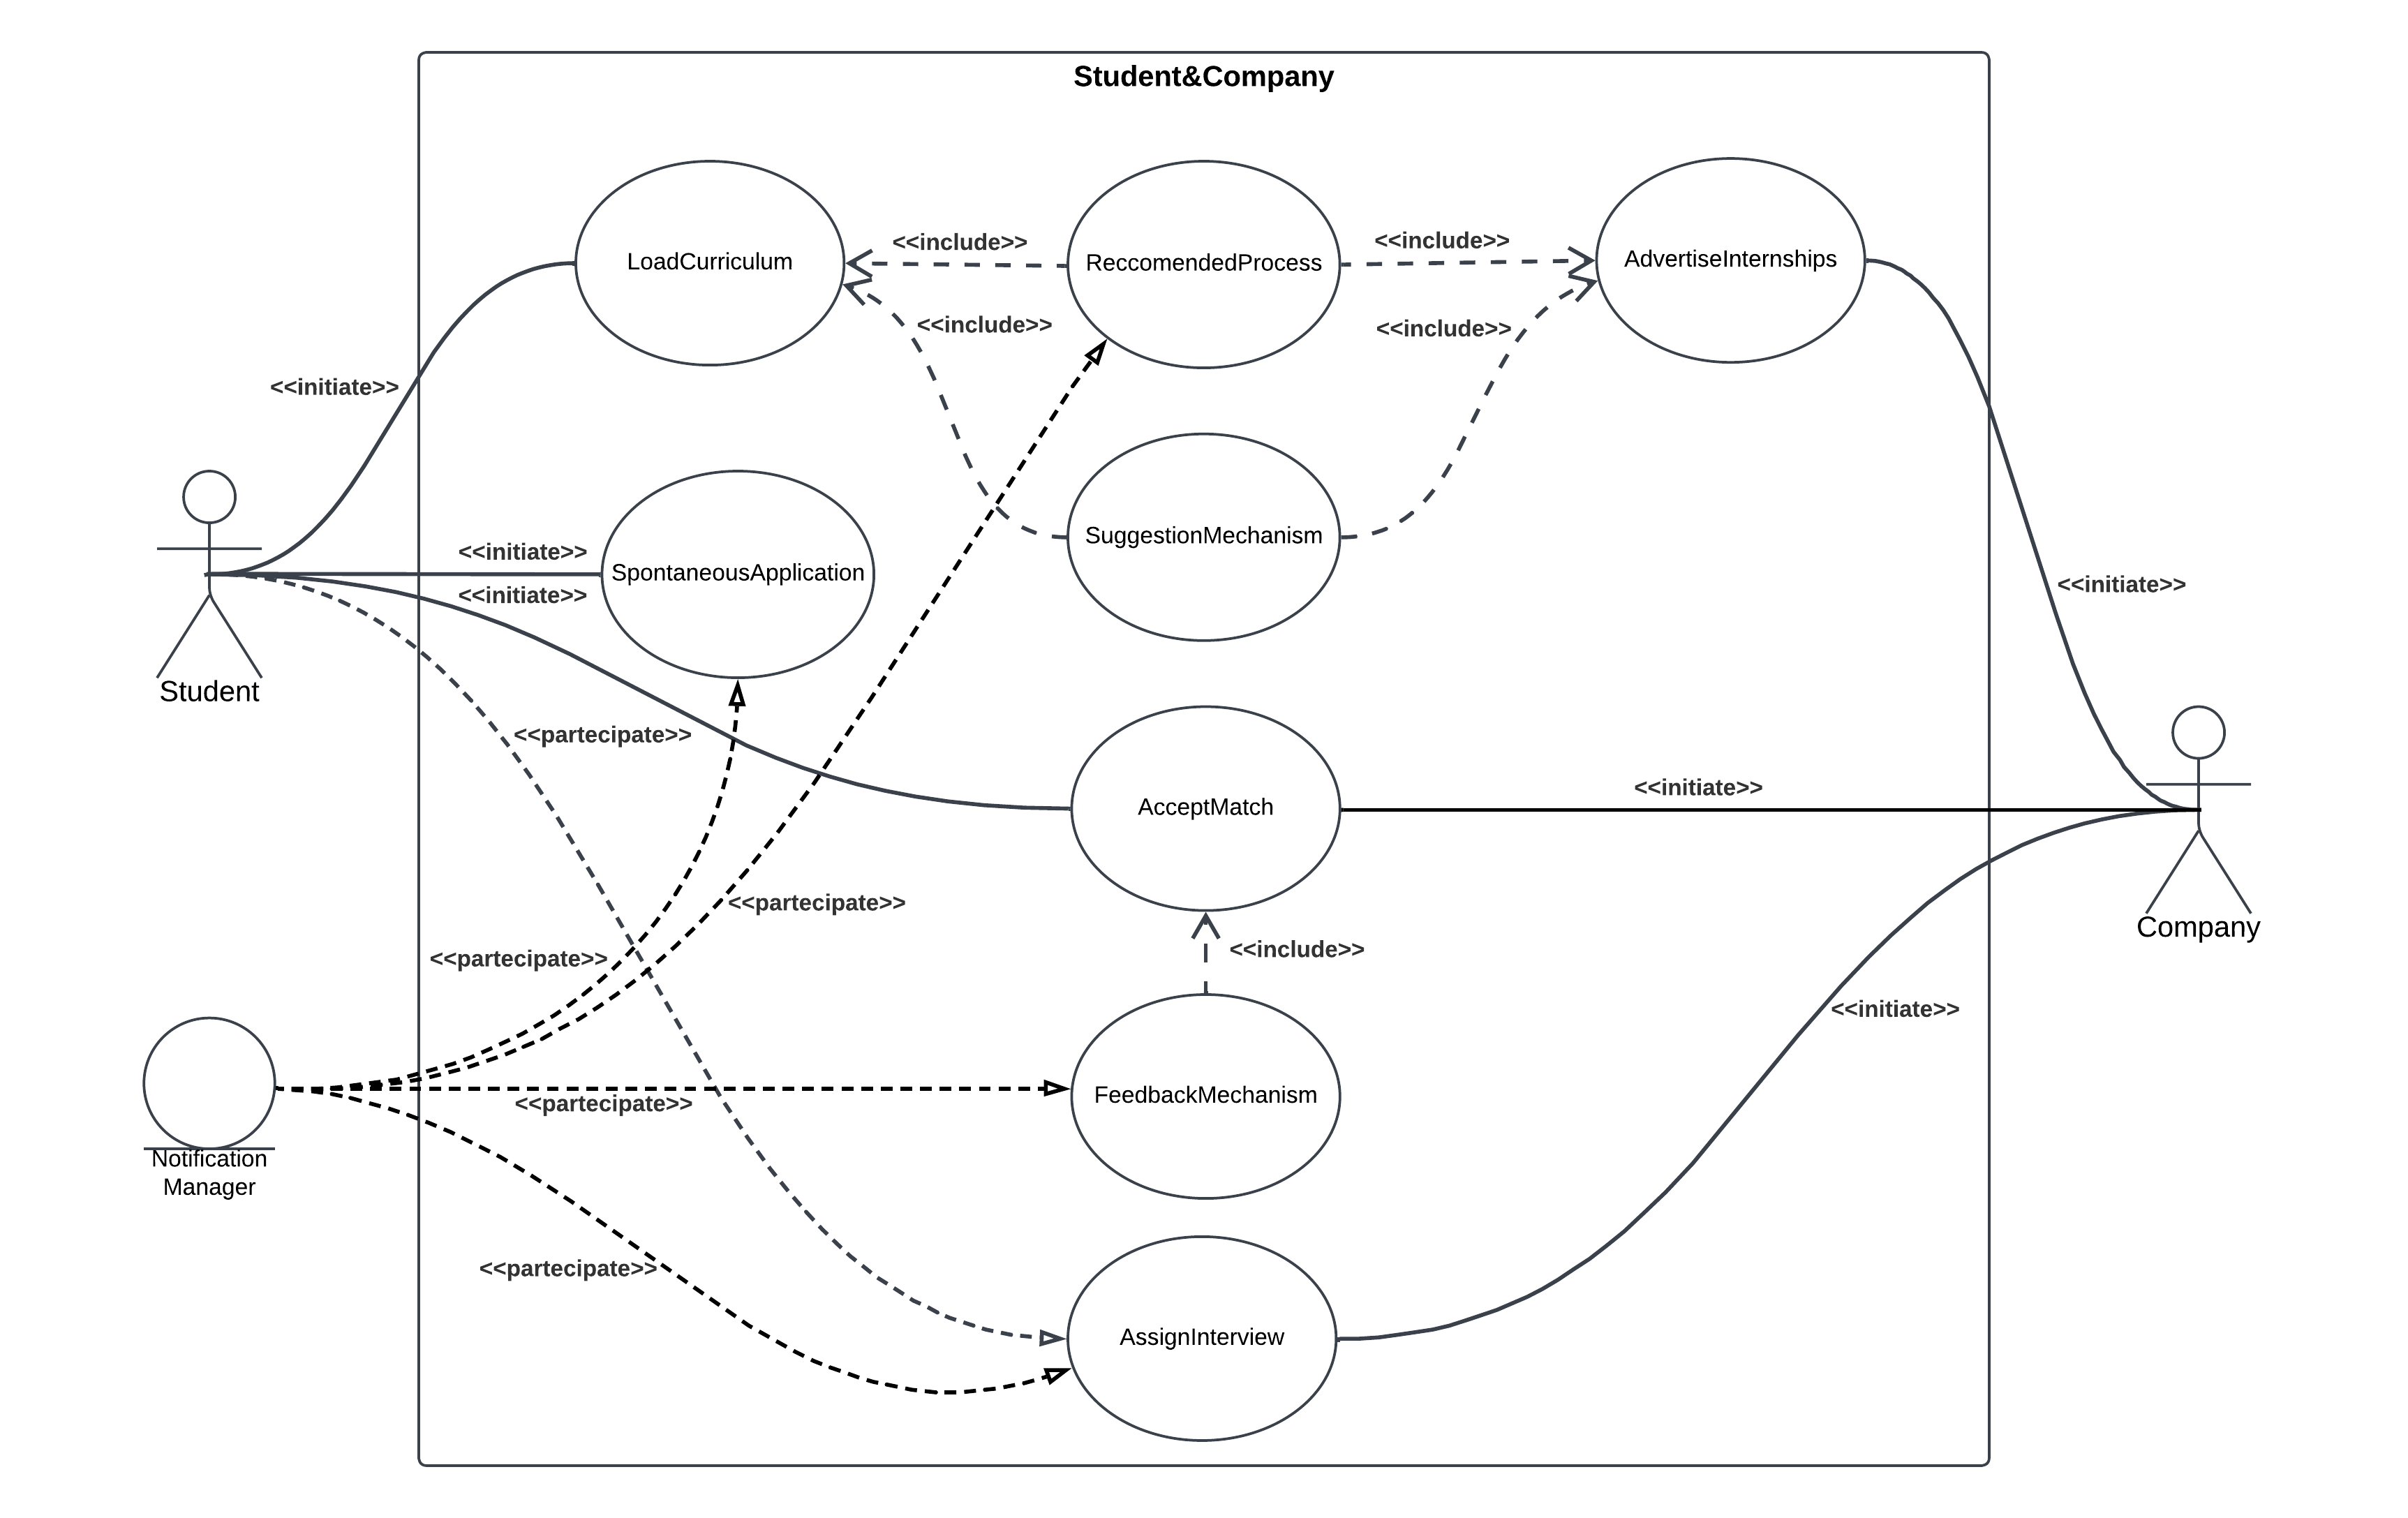
\includegraphics[width=1 \textwidth]{Latex/Images/RASD/UseCases/StudentCompanyUseCase.png}
    \caption{Student and Company Use Case Diagram}
    \label{fig:StudentCompanyUseCaseDiagram}
\end{figure}
This diagram illustrates the main functionalities of the platform, such as the loading of CV or the creation of an Internship Offer. \\
This diagram both shows the different use cases that are specific to Students or Companies, and the common ones, such as the Acceptance of a Match. In such cases, the use case can be initiated by both actors.
\clearpage
\begin{figure}[H]
    \centering
    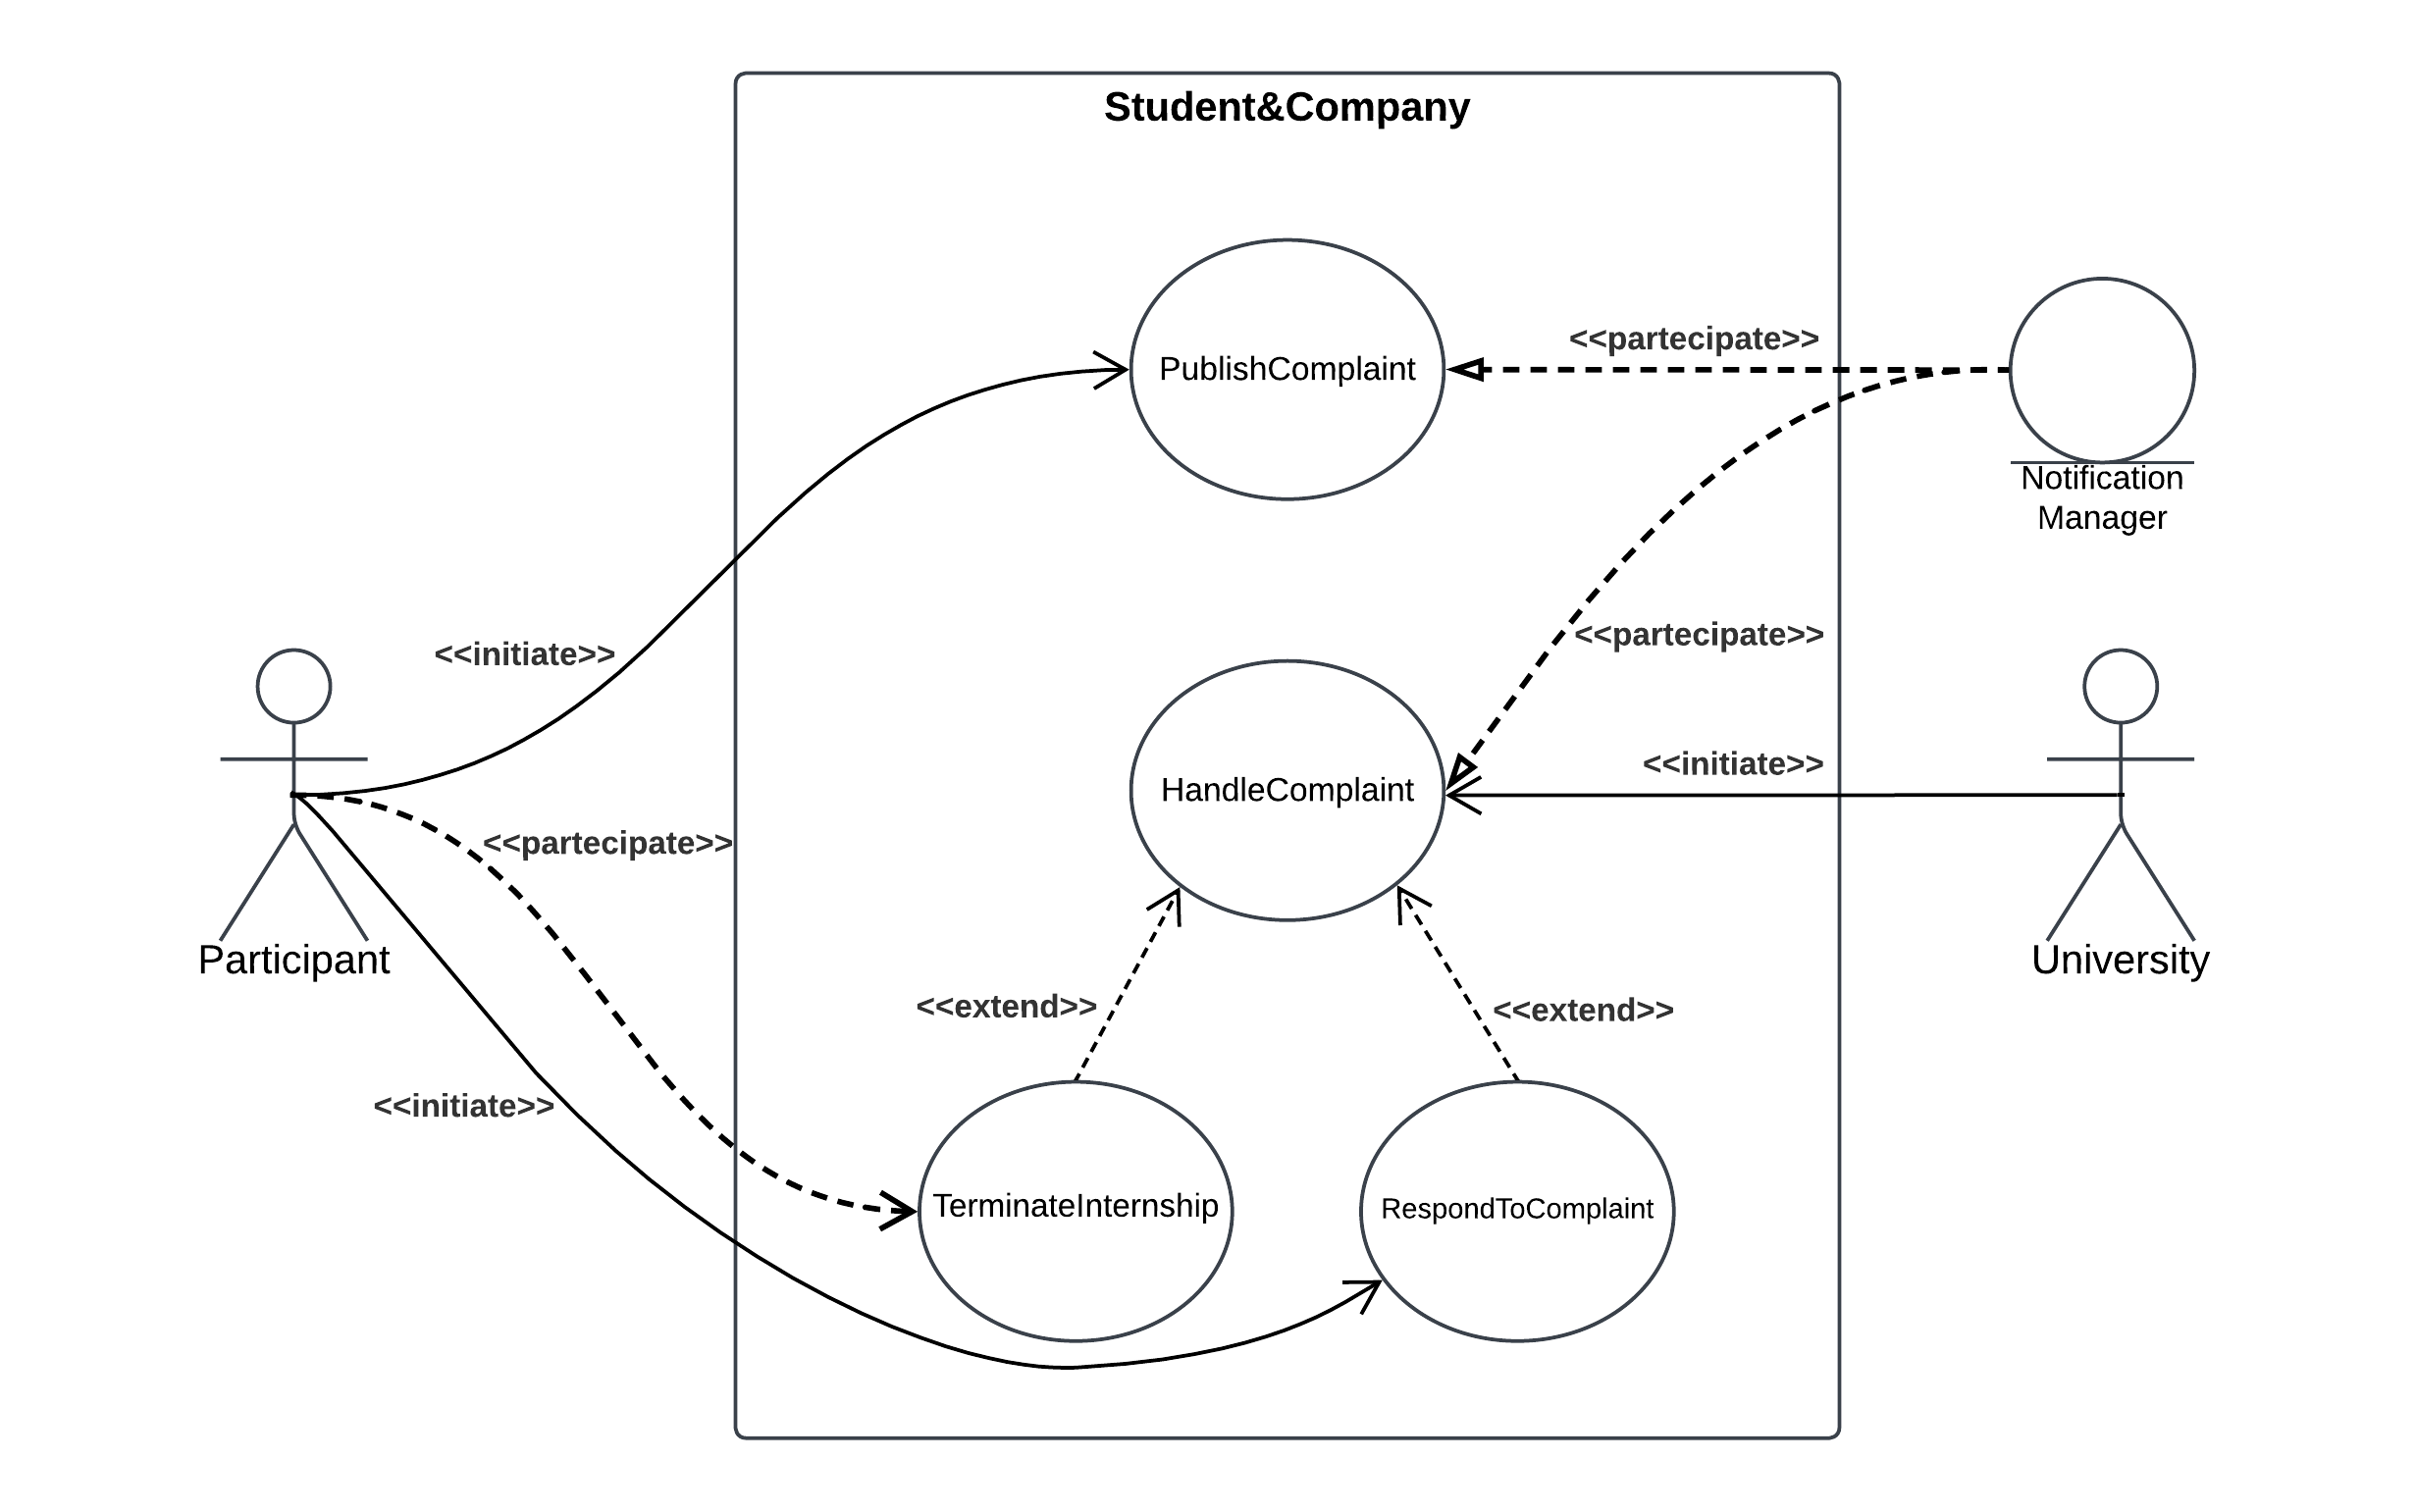
\includegraphics[width=1 \textwidth]{Latex/Images/RASD/UseCases/UniversityUseCaseDiagram.png}
    \caption{University and Complaint Use Case Diagram}
    \label{fig:UniveristyUseCaseDiagram}
\end{figure}
This diagram concentrates on the functionalities offered to Universities. It shows how a Participant can create a Complaint, and how the University can handle it. \\
More importantly, it shows that a complaint can be handled “as is” by the University, or it can be extended either by the other Participants that respond to such complaint or by the University itself that can interrupt an Ongoing Internship.
\clearpage

\subsubsection{Use Cases}

\begin{table}[H]
    \centering
    \begin{tabular}{|p{3cm}|p{12cm}|}
    \hline
    \multicolumn{2}{|c|}{\textbf{RegisterStudent}} \\ \hline
    Actor & 
    \begin{itemize}
        \item Student
        \item Email Provider
    \end{itemize} \\ \hline
    Entry Condition & The user is not logged in. \\ \hline
    Event Flow & 
    \begin{enumerate}         
        \item The Student presses the “Sign up” button situated on the dashboard.
        \item The platform opens the sign-up page.
        \item The Student selects the “Student” option, provides the required information (name, surname, date of birth, institutional email, optionally personal email, password, University name among those available) and click the “Sign Up” button.
        \item The platform validates the email and checks if it is unique.
        \item The platform registers the Student and sends a confirmation email to the provided email address through the Email Provider.
        \item The platform shows a message to the Student to confirm the registration.
        \item The Student confirms the registration by clicking on the link in the email.
        \item The platform confirms the registration and activates the account.
        \item The Student is redirected to the platform's dashboard.
    \end{enumerate} \\ \hline
    Exit Condition & The Student is registered and logged in. \\ \hline
    Exception & 
    \begin{itemize}
        \item The Student provides incorrect information.
        \item The Student does not confirm the registration.
        \item The email is already in use.
    \end{itemize} \\ \hline
    \end{tabular}
    \caption{[UC1]: Student registration use case}
    \label{tab:UC1}
\end{table}
\clearpage
\begin{table}[H]
    \centering
    \begin{tabular}{|p{3cm}|p{12cm}|}
    \hline
    \multicolumn{2}{|c|}{\textbf{RegisterCompany}} \\ \hline
    Actor & 
    \begin{itemize}
        \item Company
        \item Email Provider
    \end{itemize} \\ \hline
    Entry Condition & The user is not logged in \\ \hline
    Event Flow &
    \begin{enumerate}         
        \item The Company presses the “Sign up” button situated on the dashboard.
        \item The platform open the sign-up page.
        \item The Company selects the “Company” option, provides the required information (Company name, Company headquarters address, VAT number, email, and password) and click the “Sign Up” button.
        \item The platform checks if the VAT number and the email are unique
        \item The platform sends a confirmation email to the provided email address through the Email Provider.
        \item The platform shows a message to the Company to confirm the registration.
        \item The Company confirms the registration by clicking on the link in the email.
        \item The platform confirms the registration and activates the account.
        \item The Company is redirected to the platform's Dashboard.
    \end{enumerate} \\ \hline
    Exit Condition & The Company is registered and logged in. \\ \hline
    Exception & 
    \begin{itemize}
        \item The Company provides incorrect information.
        \item The Company does not confirm the registration.
        \item The VAT number or the email is already in use.
    \end{itemize} \\ \hline
    \end{tabular}
    \caption{[UC2]: Company registration use case}
    \label{tab:UC2}
\end{table}

\begin{table}[H]
    \centering
    \begin{tabular}{|p{3cm}|p{12cm}|}
    \hline
    \multicolumn{2}{|c|}{\textbf{RegisterUniversity}} \\ \hline
    Actor & 
    \begin{itemize}
        \item University
        \item Email Provider
    \end{itemize} \\ \hline
    Entry Condition & The user is not logged in. \\ \hline
    Event Flow &
    \begin{enumerate}         
        \item The University presses the “Sign up” button situated on the dashboard.
        \item The platform open the sign-up page.
        \item The University selects the “University” option, provides the required information (University Name, University description, VAT number, email of the University office that will manage the internship program, and password) and click the “Sign Up” button.
        \item The platform checks if the VAT number and the email are unique
        \item The platform sends a confirmation email to the provided email address through the Email Provider.
        \item The platform shows a message to the University to confirm the registration.
        \item The University confirms the registration by clicking on the link in the email.
        \item The platform confirms the registration and activates the account.
        \item The University is redirected to the platform's Dashboard.
    \end{enumerate} \\ \hline
    Exit Condition & The University is registered and logged in.\\ \hline
    Exceptions &
    \begin{itemize}
        \item The University provides incorrect information.
        \item The University does not confirm the registration.
        \item The VAT number or the email is already in use.
    \end{itemize} \\ \hline
    \end{tabular}
    \caption{[UC3]: University registration use case}
    \label{tab:UC3}
\end{table}

\begin{table}[H]
    \centering
    \begin{tabular}{|p{3cm}|p{12cm}|}
    \hline
    \multicolumn{2}{|c|}{\textbf{LoginUser}} \\ \hline
    Actor & 
    \begin{itemize}
        \item User
    \end{itemize}\\ \hline
    Entry Condition & The user is not logged in \\ \hline
    Event Flow &
    \begin{enumerate}         
        \item The User presses the “Sign in” button situated on the dashboard.
        \item The platform open the sign-in page.
        \item The user provides their email and password.
        \item The platform validates the credentials.
        \item The platform confirms the credentials and logs in the User.
        \item The User is redirected to the platform's Dashboard.
    \end{enumerate} \\ \hline
    Exit Condition & The User is logged in. \\ \hline
    Exceptions &
    \begin{itemize}
        \item The User provides incorrect email or password.
    \end{itemize} \\ \hline
    \end{tabular}
    \caption{[UC4]: User login use case}
    \label{tab:UC4}
\end{table}

\begin{table}[H]
    \centering
    \begin{tabular}{|p{3cm}|p{12cm}|}
    \hline
    \multicolumn{2}{|c|}{\textbf{LoadCurriculum}} \\ \hline
    Actor & 
    \begin{itemize}
        \item Student
        \item Notification Manager
        \item Company
    \end{itemize}\\ \hline
    Entry Condition & The Student is logged in \\ \hline
    Event Flow &
    \begin{enumerate}         
        \item The Student presses the “CV” menu button situated on the dashboard.
        \item The platform opens the Curriculum page.
        \item The Student fills the form with the required information (current level of education, known languages, technical skills, a photo of himself, a brief description of his interests and hobbies etc...) and click the “Submit CV” button.
        \item The platform publishes the CV.
        \item The platform generates a list of matching internships based on the CV.
        \item The platform provides feedback and suggestions to improve the CV.
        \item The Student is redirected to his account page.
        \item The platform notifies the new matching Companies through the Notification Manager. 
    \end{enumerate} \\ \hline
    Exit Condition & The Student's CV is uploaded. \\ \hline
    Exception & 
    \begin{itemize} 
        \item The Student provides invalid or partial information.
    \end{itemize} \\ \hline
    \end{tabular}
    \caption{[UC5]: Student uploads Curriculum use case}
    \label{tab:UC5}
\end{table}

\begin{table}[H]
    \centering
    \begin{tabular}{|p{3cm}|p{12cm}|}
    \hline
    \multicolumn{2}{|c|}{\textbf{AdvertiseInternships}} \\ \hline
    Actor & 
    \begin{itemize}
        \item Company
        \item Notification Manager
        \item Student
    \end{itemize}\\ \hline
    Entry Condition & The Company is logged in\\ \hline
    Event Flow &
    \begin{enumerate}         
        \item The Company presses the “Internship Offers” button situated on the dashboard.
        \item The Platform opens the Internships page.
        \item The Company presses the “Create Internship” button.
        \item The platform shows the Internship creation form.
        \item The Company fills the form with the required information (Internship title, description, start date and duration, office address, required skills and benefits offered) and click the “Submit Internship” button.
        \item The platform publishes the Internship.
        \item The platform generates a list of matching Students based on the Internship.
        \item The system provides feedback and suggestions to improve the internship description.
        \item The Company is redirected to the Internships page.
        \item The platform notifies the new matching Students through the Notification Manager. 
    \end{enumerate} \\ \hline
    Exit Condition & The Internship is created and published.\\ \hline
    Exception & 
    \begin{itemize}        
        \item The Company provides invalid or partial information.
    \end{itemize} \\ \hline
    \end{tabular}
    \caption{[UC6]: Company advertises an Internship use case}
    \label{tab:UC6}
\end{table}

\begin{table}[H]
    \centering
    \begin{tabular}{|p{3cm}|p{12cm}|}
    \hline
    \multicolumn{2}{|c|}{\textbf{SpontaneousApplication}} \\ \hline
    Actor & 
    \begin{itemize}
        \item Student
        \item Company
        \item Notification Manager
    \end{itemize}\\ \hline
    Entry Condition & The Student is logged in and has his CV uploaded. \\ \hline
    Event Flow &
    \begin{enumerate}         
        \item The Student presses the “Browse Internships” button situated on the dashboard.
        \item The platform opens the global Internships page.
        \item The Student presses the “Apply” button on one of the available Internships.
        \item The platform adds the application to the Company and Student list of applications.
        \item The platform notifies the Company of the Spontaneous Application through the Notification Manager.
    \end{enumerate} \\ \hline
    Exit Condition & The application is successfully submitted to the Company.\\ \hline
    Exception & 
    \begin{itemize}       
        \item Internship is no longer available.
    \end{itemize} \\ \hline
    \end{tabular}
    \caption{[UC7]: Student submits Spontaneous Application use case}
    \label{tab:UC7}
\end{table}

\begin{table}[H]
    \centering
    \begin{tabular}{|p{3cm}|p{12cm}|}
    \hline
    \multicolumn{2}{|c|}{\textbf{AcceptMatch}} \\ \hline
    Actor & 
    \begin{itemize}
        \item Participant
        \item Notification Manager
    \end{itemize}\\ \hline
    Entry Condition & A Match is generated between the Student and the Company's Internship and the Student has his CV uploaded. \\ \hline
    Event Flow &  
    \begin{enumerate}
        \item The Participant presses the “Recommendations Process” button situated on the dashboard.
        \item The platform opens the respective Recommendations pages.
        \item The Participant accepts the Match.
        \item The platform stores the result.
        \item If the other party has already accepted the Match, the platform adds the Interview to the Student and the Company's list of Interviews and notifies both parties through the Notification Manager.
    \end{enumerate} \\ \hline
    Exit Condition & The Match is successfully accepted by the participant.\\ \hline
    Exception & 
    \begin{itemize}
        \item None
    \end{itemize} \\ \hline
    \end{tabular}
    \caption{[UC8]: Company or Student accepts Match use case}
    \label{tab:UC8}
\end{table}

\begin{table}[H]
    \centering
    \begin{tabular}{|p{3cm}|p{12cm}|}
    \hline
    \multicolumn{2}{|c|}{\textbf{FeedbackMechanism}} \\ \hline
    Actor & 
    \begin{itemize}
        \item Participant
    \end{itemize}\\ \hline
    Entry Condition & The Participant is logged in. \\ \hline
    Event Flow &      
    \begin{enumerate}         
        \item The Participant presses the “Recommendations Process” button situated on the dashboard.
        \item The platform opens the respective Recommendations pages.
        \item The Participant accept or decline the Match.
        \item The platform asks for feedback about the Match.
        \item The Participant submits the feedback.
        \item The platform stores the feedback.
    \end{enumerate} \\ \hline
    Exit Condition & Feedback is successfully provided. \\ \hline
    Exception & 
    \begin{itemize}     
        \item None
    \end{itemize} \\ \hline
    \end{tabular}
    \caption{[UC9]: Feedback is asked upon Match result use case}
    \label{tab:UC9}
\end{table}

\begin{table}[H]
    \centering
    \begin{tabular}{|p{3cm}|p{12cm}|}
    \hline
    \multicolumn{2}{|c|}{\textbf{SuggestionMechanism}} \\ \hline
    Actor & 
    \begin{itemize}
        \item Participant
    \end{itemize}\\ \hline
    Entry Condition & A Student has uploaded his CV or a Company has created an Internship.\\ \hline
    Event Flow & 
    \begin{enumerate}         
        \item The platform analyses the Student's CV or the Company's Internship.
        \item The platform generates a list of suggestions to improve the CV or the Internship description.
        \item The platform displays a notification on the Participant's dashboard page.
        \item The Participant open the notification.
        \item The platform displays the suggestions.
    \end{enumerate} \\ \hline
    Exit Condition & Suggestions are successfully provided. \\ \hline
    Exception & 
    \begin{itemize}        
        \item No valuable suggestions are found.  
    \end{itemize} \\ \hline
    \end{tabular}
    \caption{[UC10]: Suggestion mechanism use case}
    \label{tab:UC10}
\end{table}

\begin{table}[H]
    \centering
    \begin{tabular}{|p{3cm}|p{12cm}|}
    \hline
    \multicolumn{2}{|c|}{\textbf{AssignInterview}} \\ \hline
    Actor & 
    \begin{itemize}
        \item Company
        \item Student
        \item Notification Manager
    \end{itemize} \\ \hline
    Entry Condition & A Match is accepted by both parties or the Company has accepted a Spontaneous Application. \\ \hline
    Event Flow &      
    \begin{enumerate}         
        \item The Company presses the “Interviews” button situated on the dashboard.
        \item The platform opens the Interviews page.
        \item The Company selects an Interview in the “ToBeSubmitted” state.
        \item The platform shows the Interview creation form.
        \item The Company fills the form with the required information (open and closed questions, deadline and additional infos) and click the “Submit Interview” button.
        \item The platform sends the form to the Student, updates his Interview status and notifies him thorough the Notification Manager.
        \item The Company is redirected to the Interviews page.
    \end{enumerate} \\ \hline
    Exit Condition & The Interview is created and submitted to the Student. \\ \hline
    Exception & 
    \begin{itemize}         
        \item None
    \end{itemize} \\ \hline
    \end{tabular}
    \caption{[UC11]: Company assigns Interview to Student use case}
    \label{tab:UC11}
\end{table}

\begin{table}[H]
    \centering
    \begin{tabular}{|p{3cm}|p{12cm}|}
    \hline
    \multicolumn{2}{|c|}{\textbf{PublishComplaint}} \\ \hline
    Actor & 
    \begin{itemize}
        \item Company
        \item Student
        \item University
        \item Notification Manager
    \end{itemize} \\ \hline
    Entry Condition & There is an Ongoing Internship between the relative Company and Student.\\ \hline
    Event Flow &      
    \begin{enumerate}         
        \item The Company presses the “Communications” button situated on the dashboard.
        \item The platform opens the Communications page.
        \item The Company presses the “Create Complaint” button.
        \item The platform shows the Complaint creation form.
        \item The Company fills the form with the required information (Student's name, Internship title, description of the problem) and click the “Submit Complaint” button.
        \item The platform publishes the Complaint.
        \item The platform notifies the Student and the University through the Notification Manager.
    \end{enumerate} \\ \hline
    Exit Condition & The Complaint is created and published. \\ \hline
    Exception & 
    \begin{itemize}       
        \item None
    \end{itemize} \\ \hline
    \end{tabular}
    \caption{[UC12]: Company publishes Complaint use case}
    \label{tab:UC12}
\end{table}

\begin{table}[H]
    \centering
    \begin{tabular}{|p{3cm}|p{12cm}|}
    \hline
    \multicolumn{2}{|c|}{\textbf{RespondToComplaint}} \\ \hline
    Actor & 
    \begin{itemize}
        \item User
        \item Notification Manager
    \end{itemize} \\ \hline
    Entry Condition & The User has an active Complaint.\\ \hline
    Event Flow &      
    \begin{enumerate}         
        \item The Student or the Company presses the “Communications” button situated on the dashboard.
        \item The platform opens the Communications page.
        \item The User presses the target complaint.
        \item The platform shows the relative Complaint page.
        \item The User responds to the Complaint and submits the message.
        \item The platform notifies the other Users involved in the Complaint about the response through the Notification Manager.
    \end{enumerate} \\ \hline
    Exit Condition & The response is successfully published, and involved Users are notified.\\ \hline
    Exception & 
    \begin{itemize}       
        \item None
    \end{itemize} \\ \hline
    \end{tabular}
    \caption{[UC13]: User responds to a Complaint use case}
    \label{tab:UC13}
\end{table}


\begin{table}[H]
    \centering
    \begin{tabular}{|p{3cm}|p{12cm}|}
    \hline
    \multicolumn{2}{|c|}{\textbf{HandleComplaint}} \\ \hline
    Actor & 
    \begin{itemize}
        \item University
        \item Student
        \item Company
    \end{itemize}\\ \hline
    Entry Condition & There is an active Complaint regarding the Company and a Student of the University.\\ \hline
    Event Flow &      
    \begin{enumerate}         
        \item The University presses the “Communications” button situated on the dashboard.
        \item The platform opens the Communications page.
        \item The University presses the target complaint.
        \item The platform shows the relative Complaint page.
        \item The University presses the “Close Complaint” button, writes a final message and submits.
        \item The platform will close the relative Complaint.
        \item The platform notifies the Student and the Company about the resolution of the Complaint through the Notification Manager.
    \end{enumerate} \\ \hline
    Exit Condition & The Complaint is closed.\\ \hline
    Exception & 
    \begin{itemize}         
        \item None
    \end{itemize} \\ \hline    
    \end{tabular}
    \caption{[UC14]: University handles Complaint use case}
    \label{tab:UC14}
\end{table}

\begin{table}[H]
    \centering
    \begin{tabular}{|p{3cm}|p{12cm}|}
    \hline
    \multicolumn{2}{|c|}{\textbf{TerminateInternship}} \\ \hline
    Actor & 
    \begin{itemize}
        \item Student
        \item Company
        \item University
        \item Notification Manager
    \end{itemize}\\ \hline
    Entry Condition & There is an active Complaint regarding the Company and a Student of the University. \\ \hline
    Event Flow & 
    \begin{enumerate}         
        \item The University presses the “Communications” button situated on the dashboard.
        \item The platform opens the Communications page.
        \item The University presses the target complaint.
        \item The platform shows the relative Complaint page.
        \item The University presses the “Interrupt Internship” button.
        \item The platform will notify the Student and the Company about the interruption of the Internship through the Notification Manager and close the relative Complaint.
    \end{enumerate} \\ \hline
    Exit Condition & The Internship is interrupted, and the Complaint is closed. \\ \hline
    Exception & 
    \begin{itemize}         
        \item None
    \end{itemize} \\ \hline  
    \end{tabular}
    \caption{[UC15]: University terminates Internship use case}
    \label{tab:UC15}
\end{table}

\subsubsection{Sequence Diagrams}
The functions used in the sequence diagrams follow these conventional meanings:
\begin{itemize}
    \item \textbf{press(Button)}: Represents the action of a user pressing Button.
    \item \textbf{submit(Content)}: Indicates a user uploading Content to the platform.
    \item \textbf{showPage(Page)}: Displays the content of a specific Page.
    \item \textbf{showError(Error)}: Displays an error message indicating an issue that occurred.
    \item \textbf{showMessage(Message)}: Displays a generic message to the user.
    \item \textbf{notify(What, Who)}: Represents a notification forwarded to the NotificationManager regarding What and intended for Who.
    \item \textbf{check()}: Verifies the validity of the information provided by the user.
    \item \textbf{update(Data)}: Refers to internal processes that update database records with Data.
\end{itemize}
For readability, in all diagrams except the first four, the user login process is omitted. It is assumed that the user is already logged in and navigating the dashboard. Accordingly, the S\&C processes are depicted as already in progress.\\

\begin{figure}[H]
    \centering
    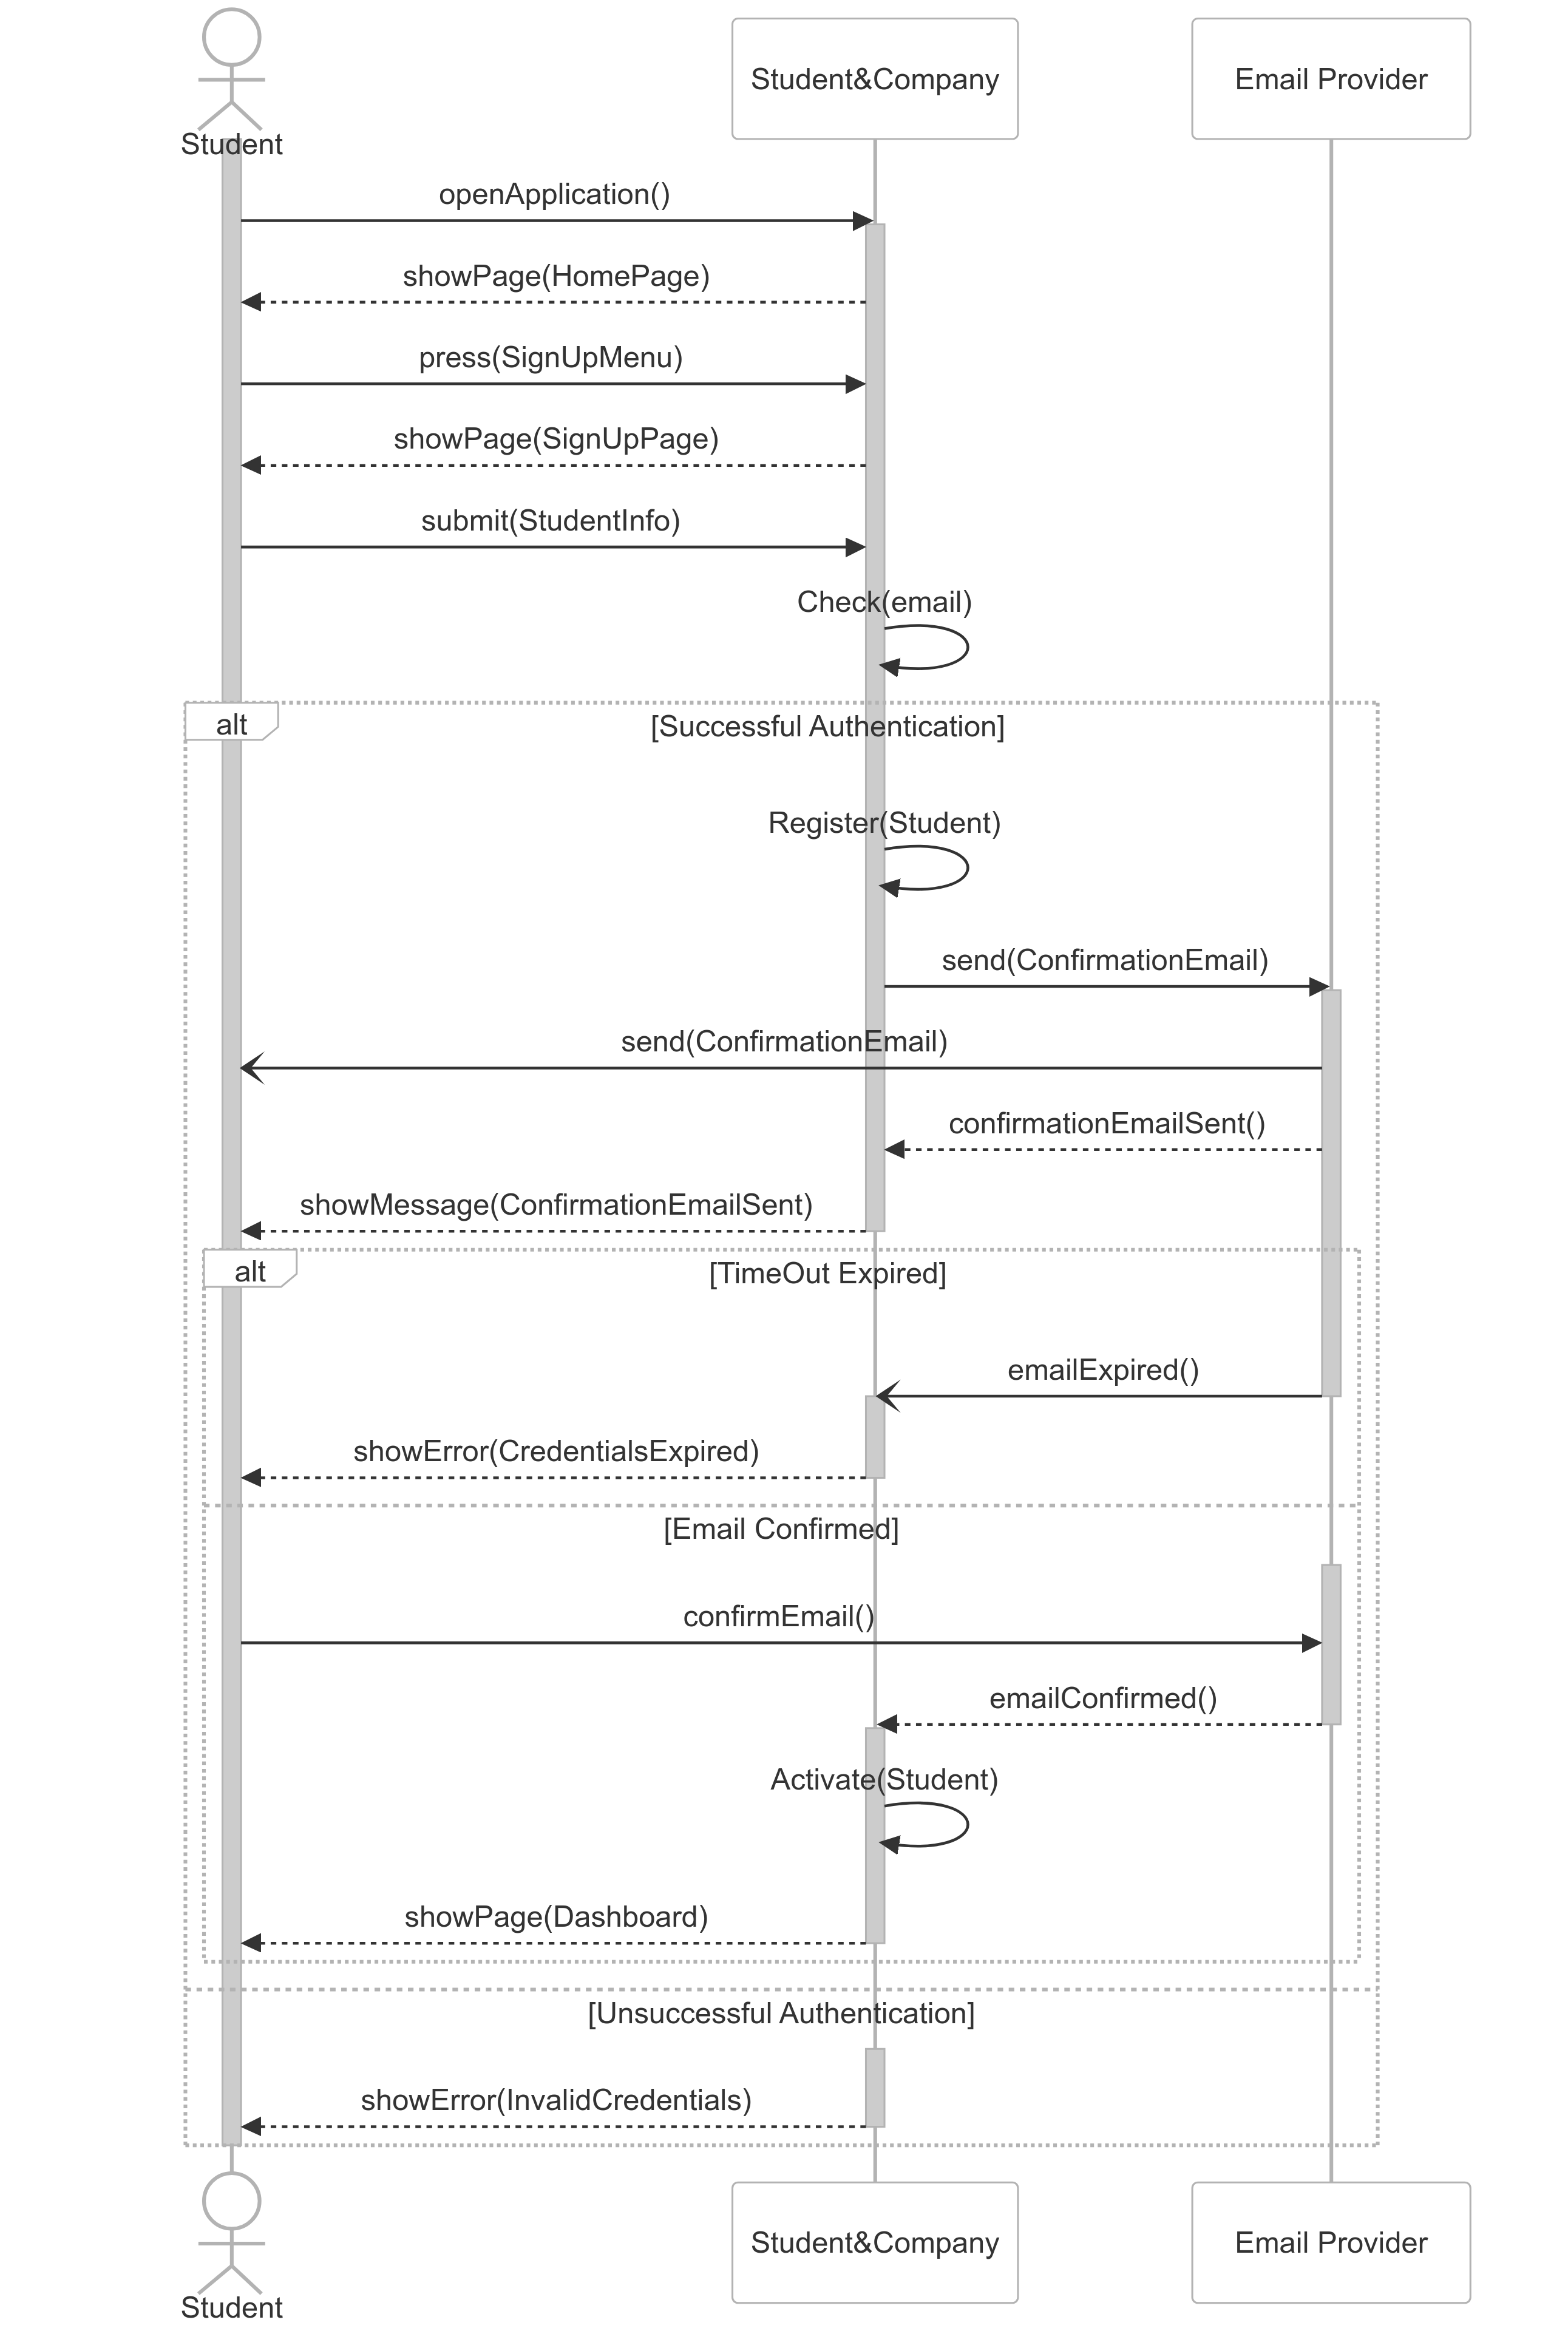
\includegraphics[width=0.75\textwidth]{Latex/Images/RASD/SequenceDiagrams/StudentSignUpSequenceDiagram.png}
    \caption{[SD1]: Student sign-up Sequence Diagram}
    \label{fig:SD1}
\end{figure}
\clearpage

\begin{figure}
    \centering
    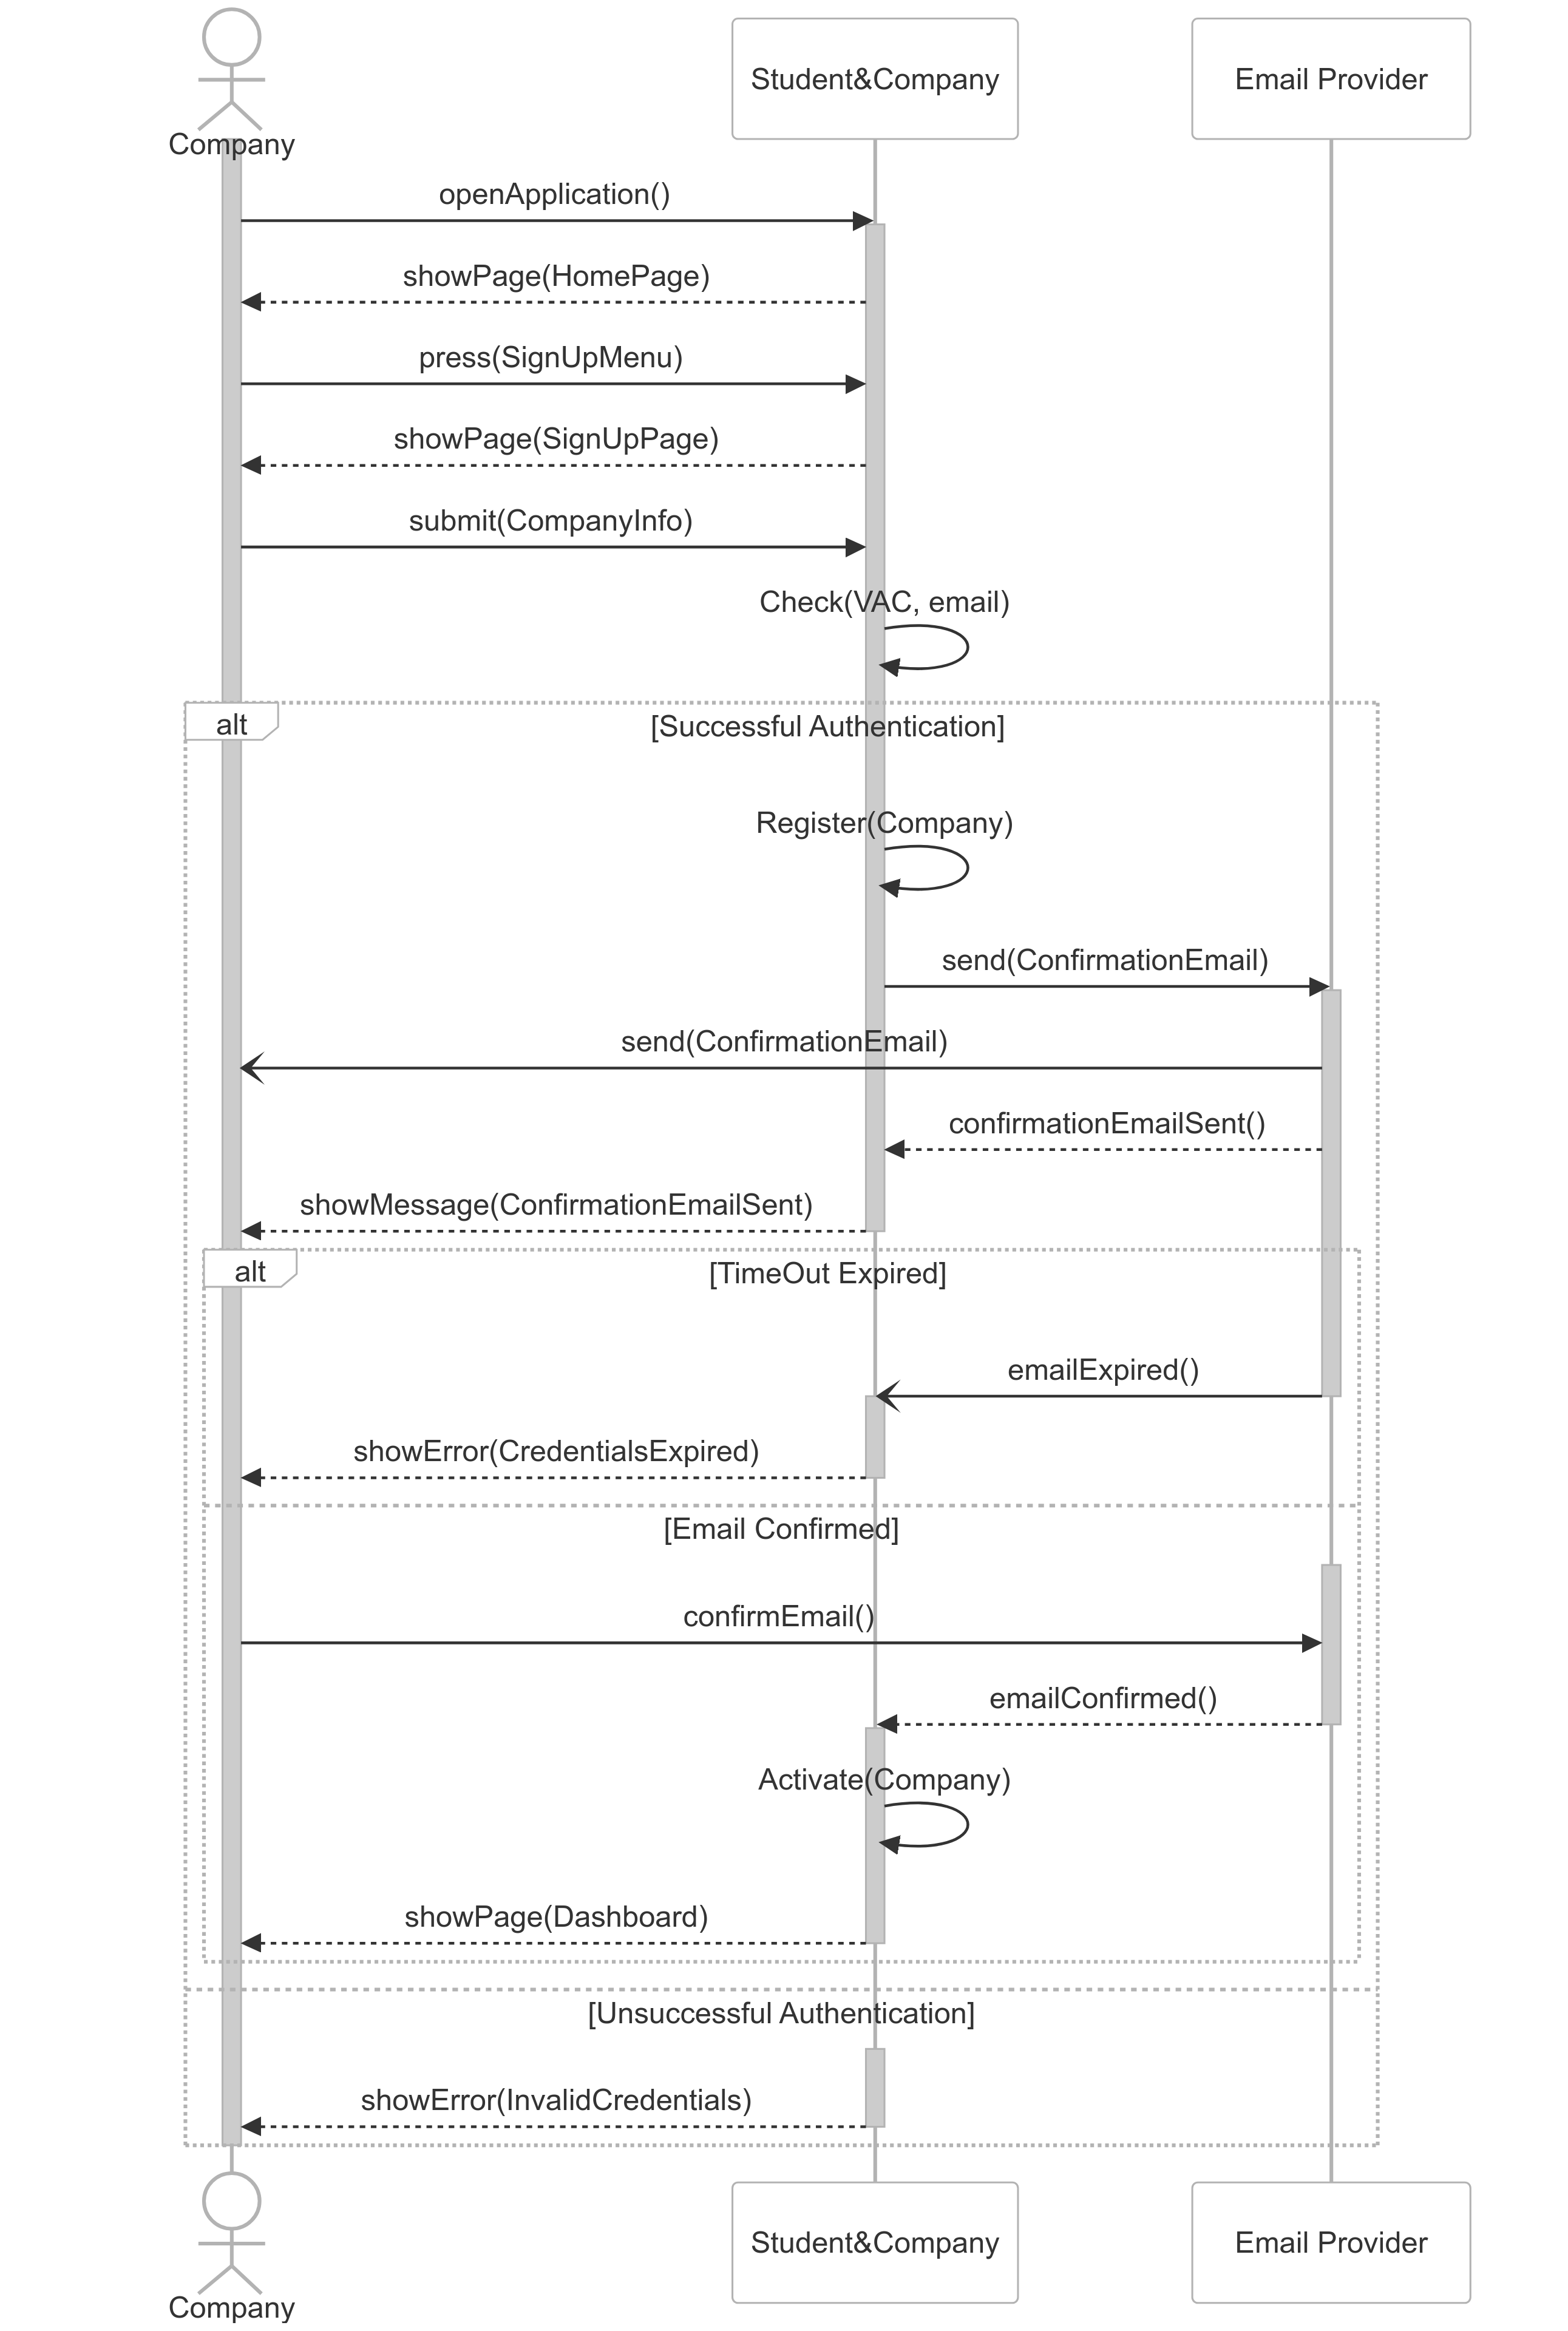
\includegraphics[width=0.8\textwidth]{Latex/Images/RASD/SequenceDiagrams/CompanySignUpSequenceDiagram.png}
    \caption{[SD2]: Company sign-up Sequence Diagram}
    \label{fig:SD2}
\end{figure}
\clearpage

\begin{figure}
    \centering
    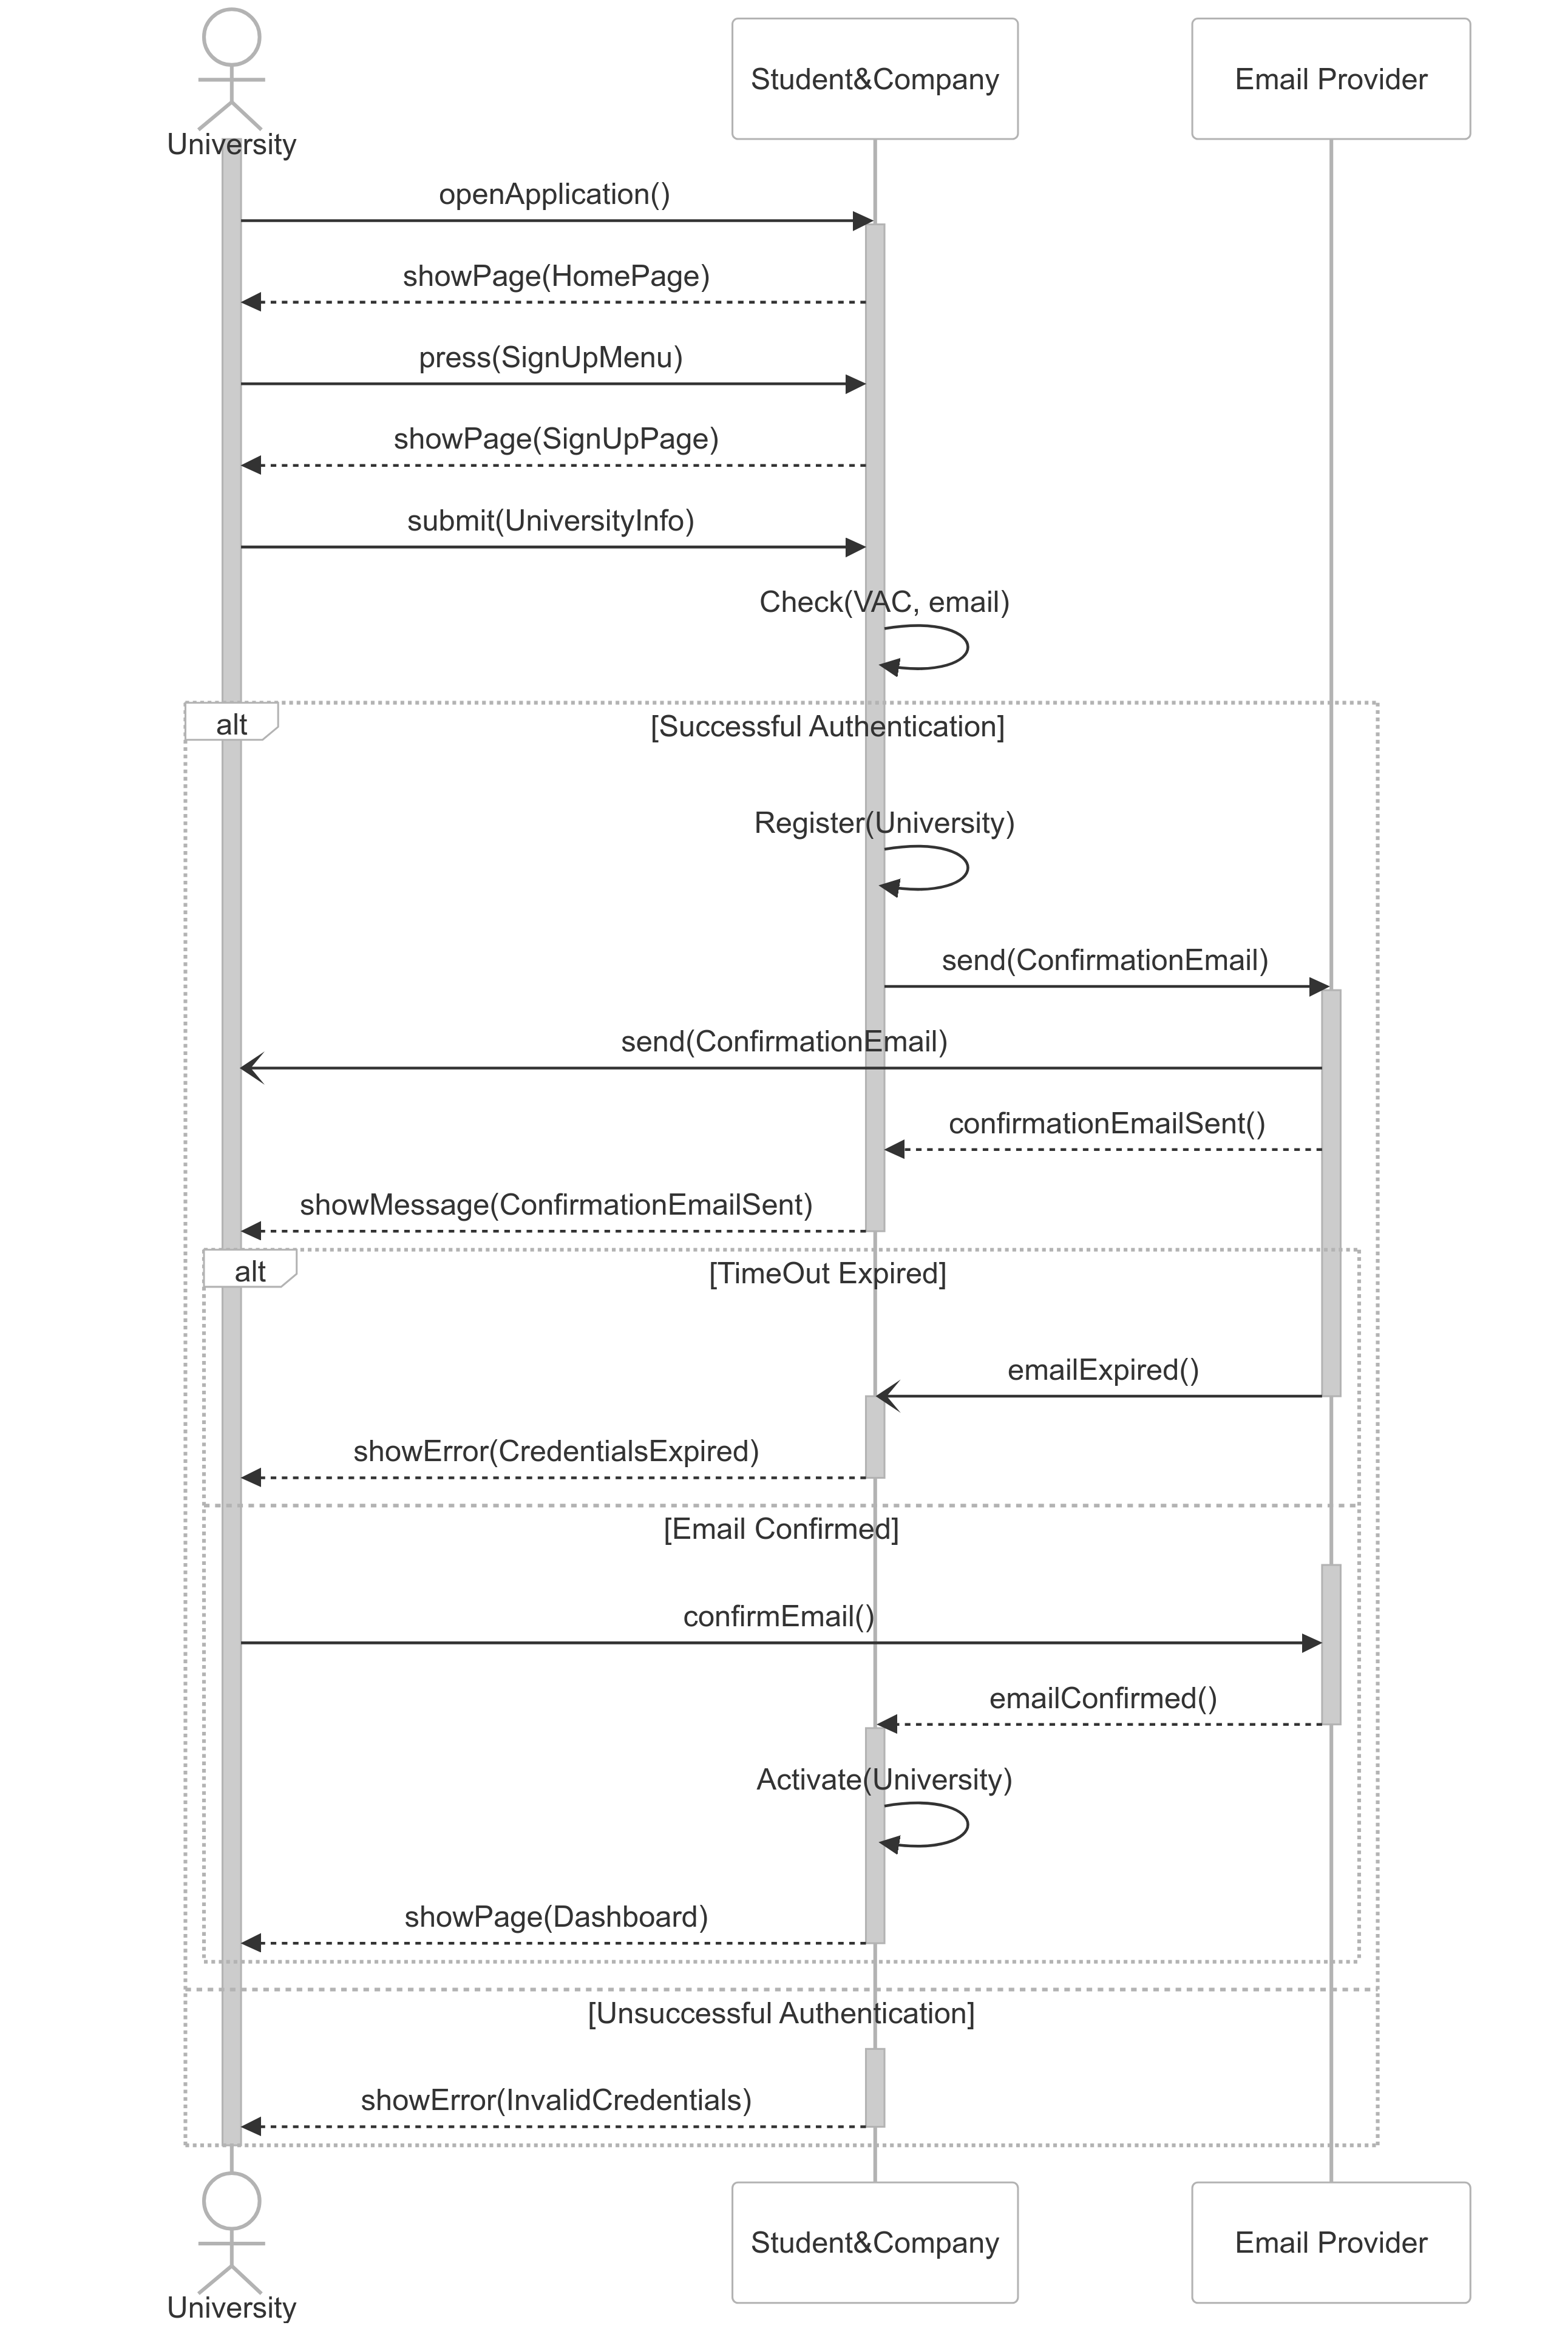
\includegraphics[width=0.8\textwidth]{Latex/Images/RASD/SequenceDiagrams/UniversitySignUpSequenceDiagram.png}
    \caption{[SD3]: University sign-up Sequence Diagram}
    \label{fig:SD3}
\end{figure}
\clearpage

\begin{figure}
    \centering
    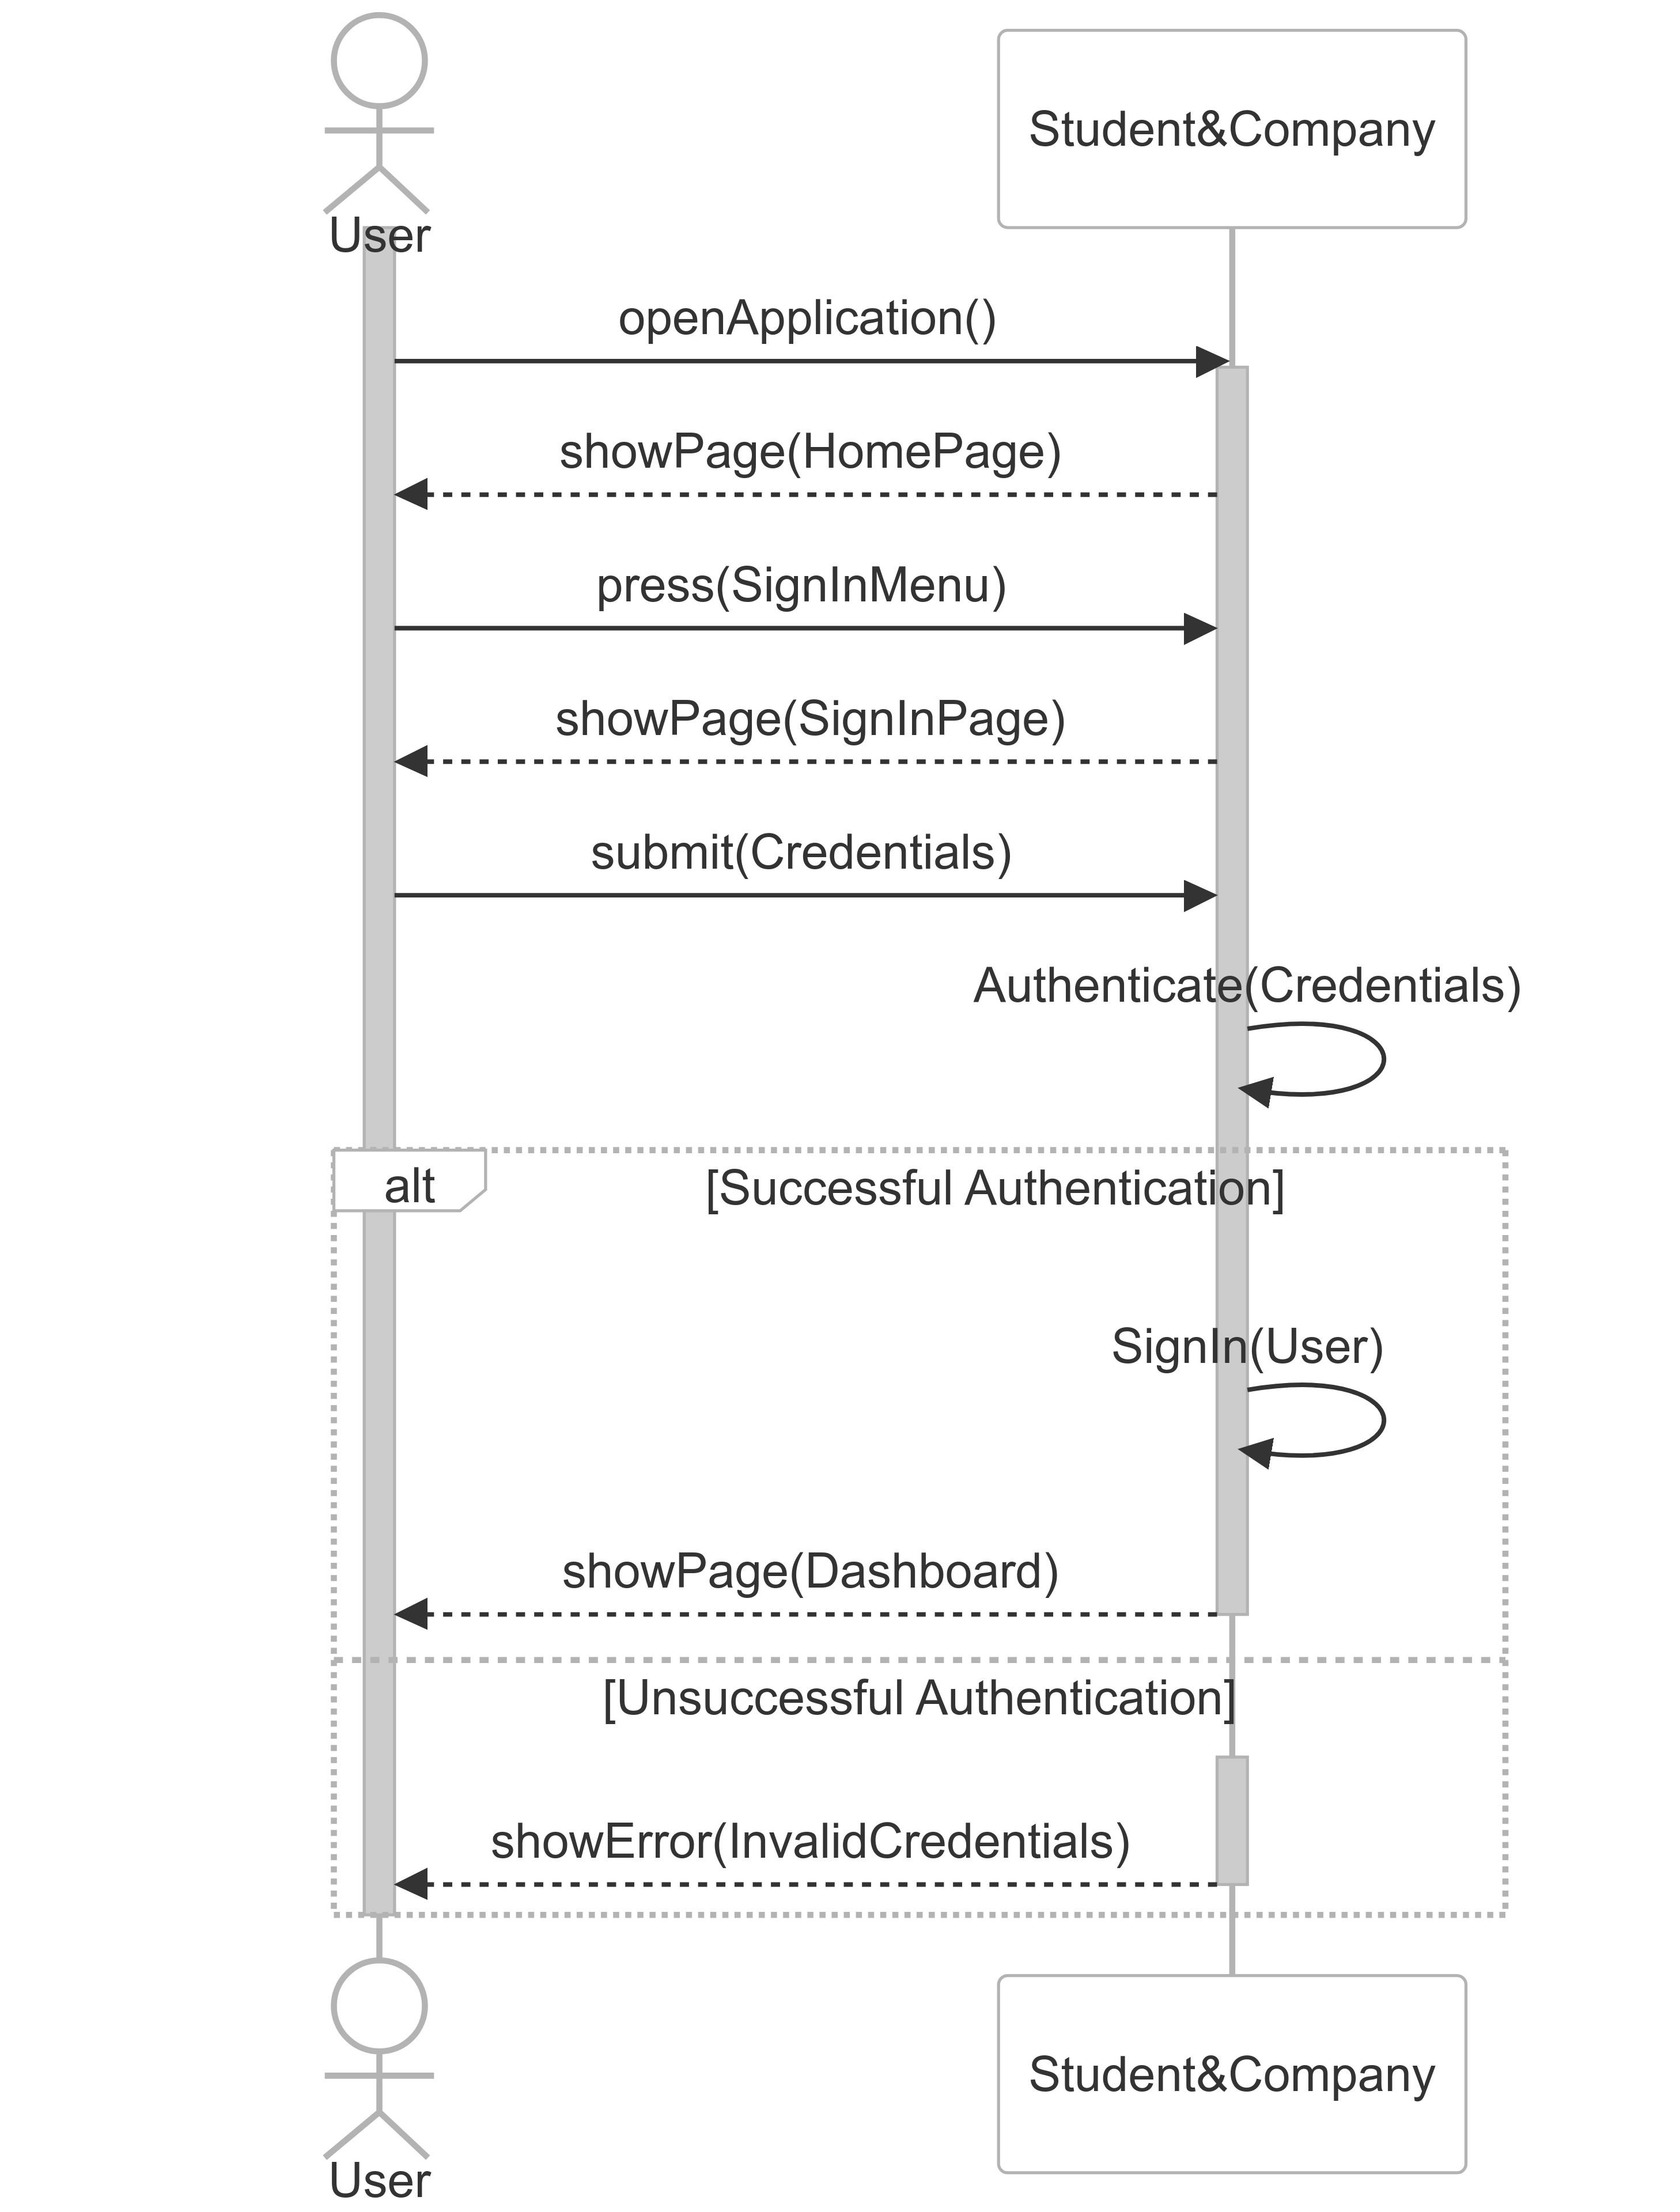
\includegraphics[width=0.6\textwidth]{Latex/Images/RASD/SequenceDiagrams/UserSignInSequenceDiagram.png}
    \caption{[SD4]: User sign-in Sequence Diagram}
    \label{fig:SD4}
\end{figure}
\clearpage

\begin{figure}
    \centering
    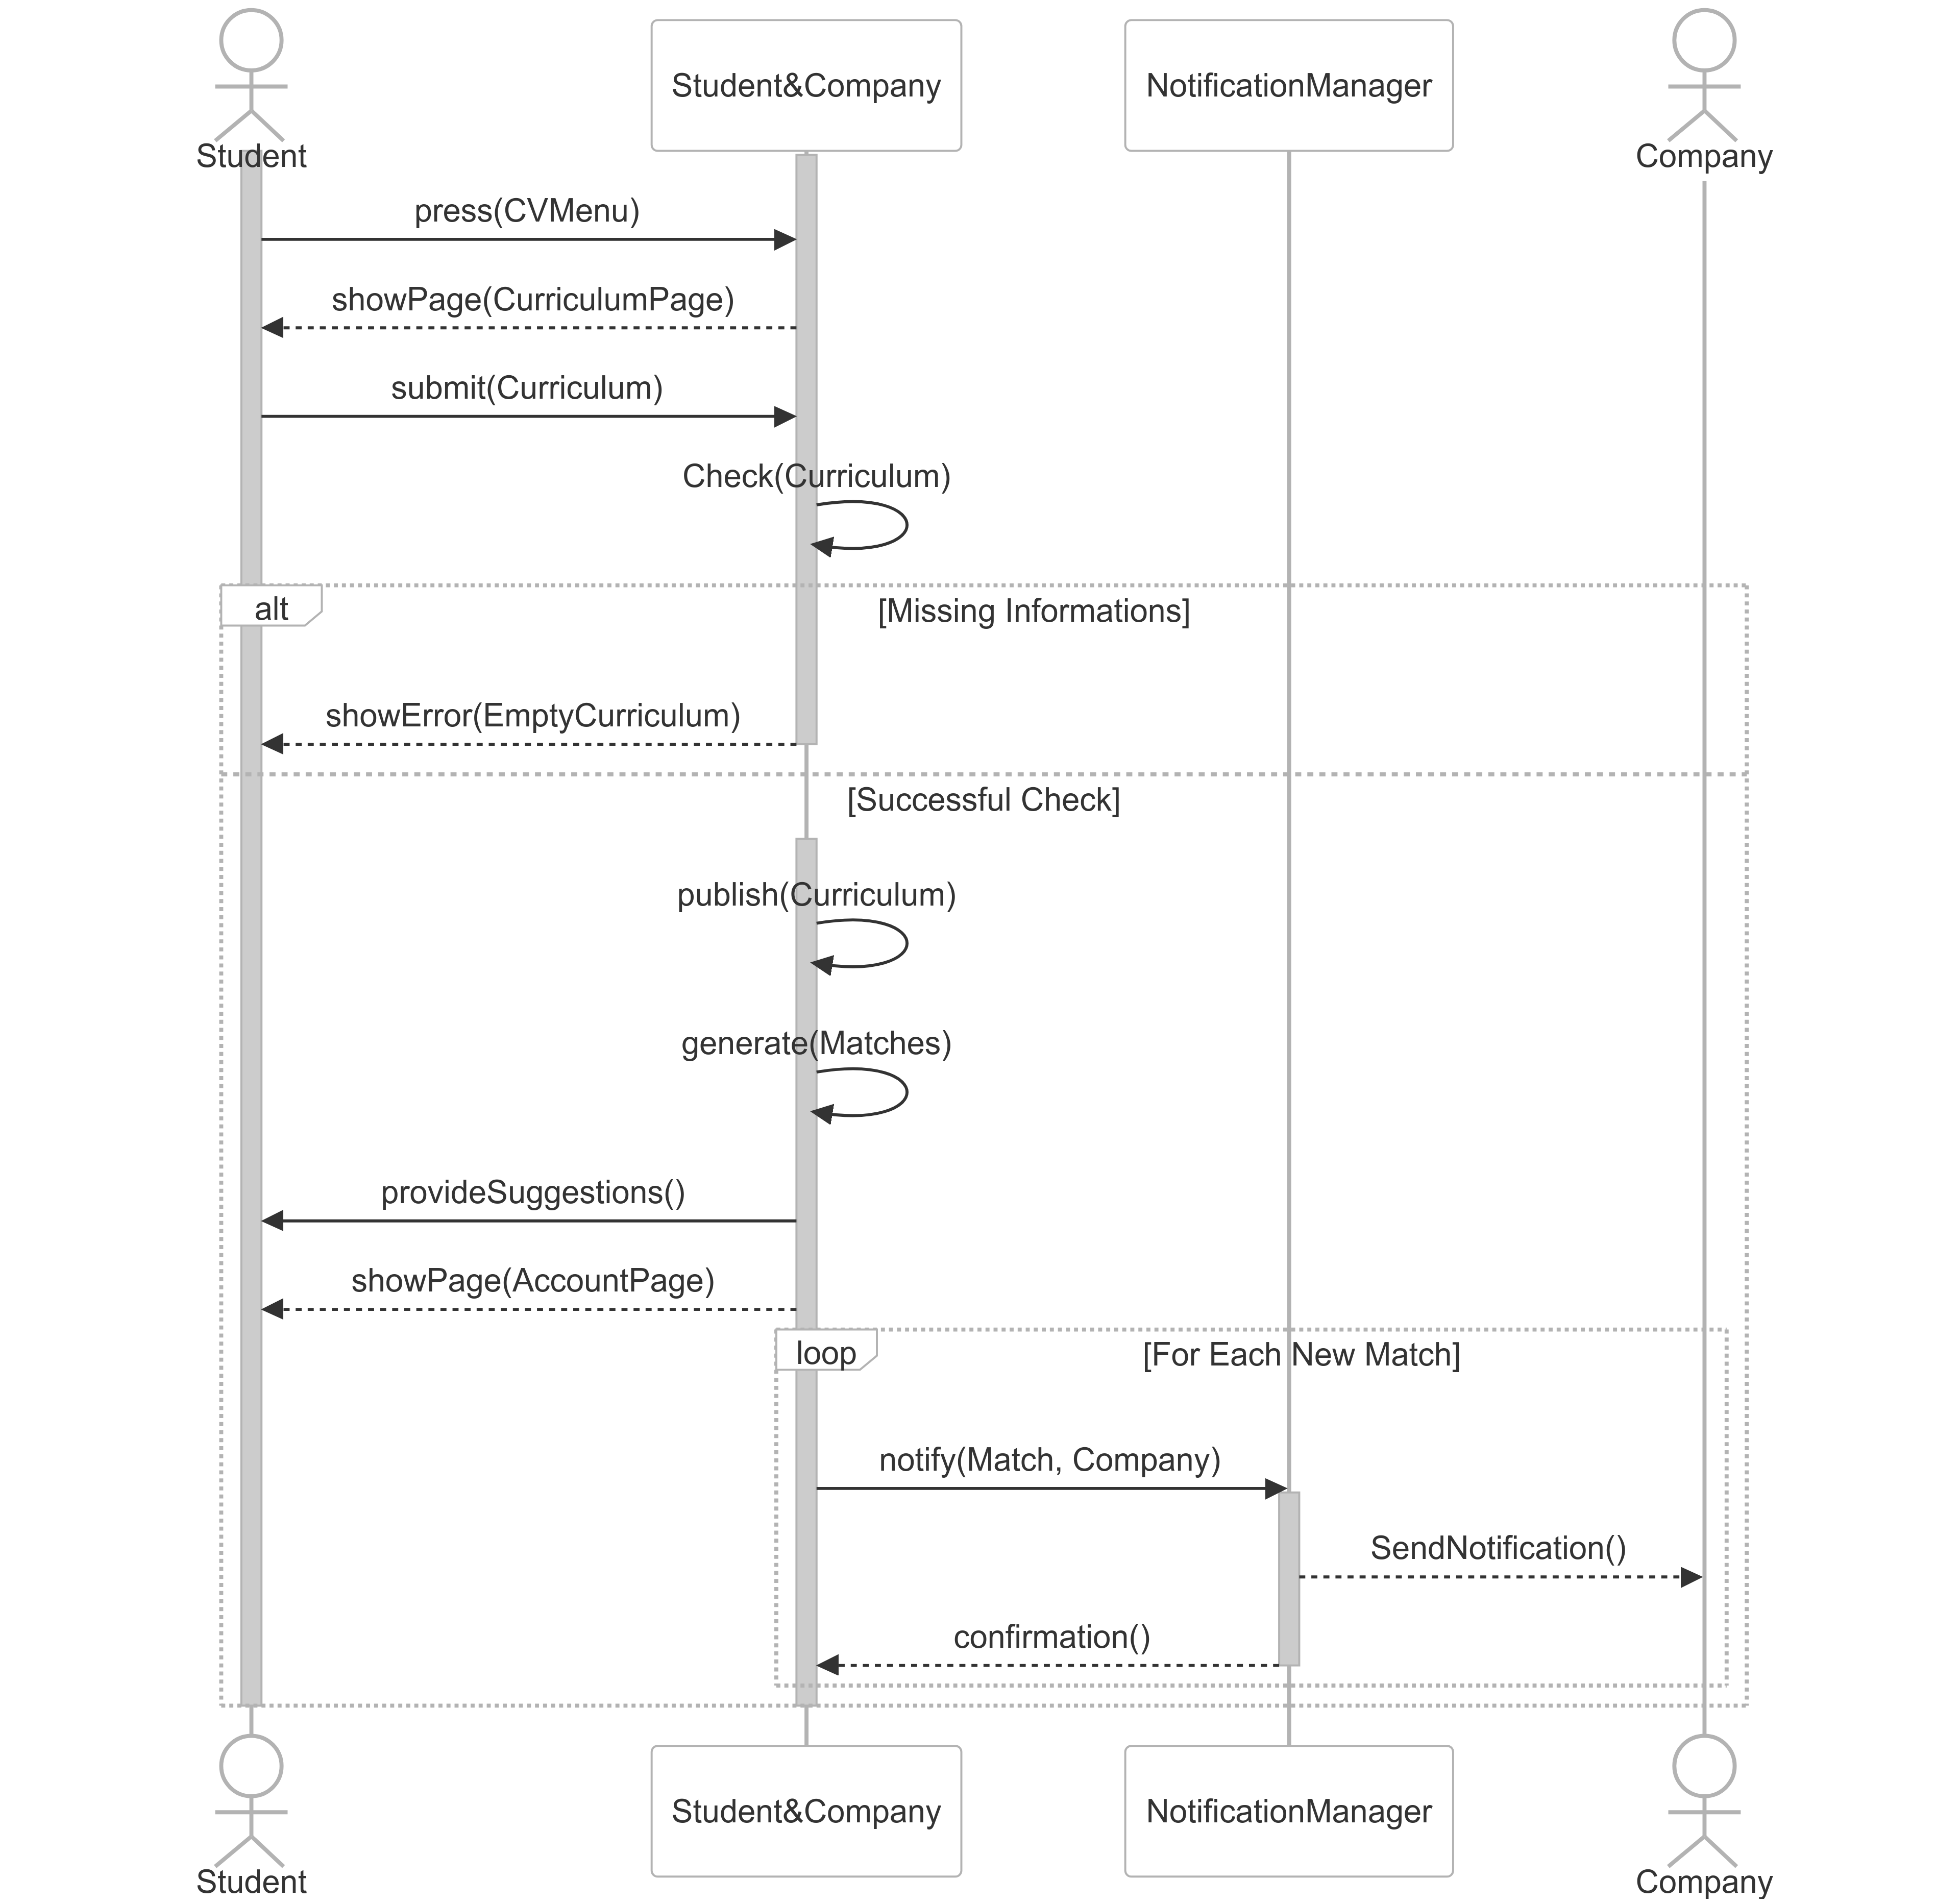
\includegraphics[width=0.8\textwidth]{Latex/Images/RASD/SequenceDiagrams/LoadCurriculumSequenceDiagram.png}
    \caption{[SD5]: Load Curriculum Sequence Diagram}
    \label{fig:SD5}
\end{figure}
\clearpage

\begin{figure}
    \centering
    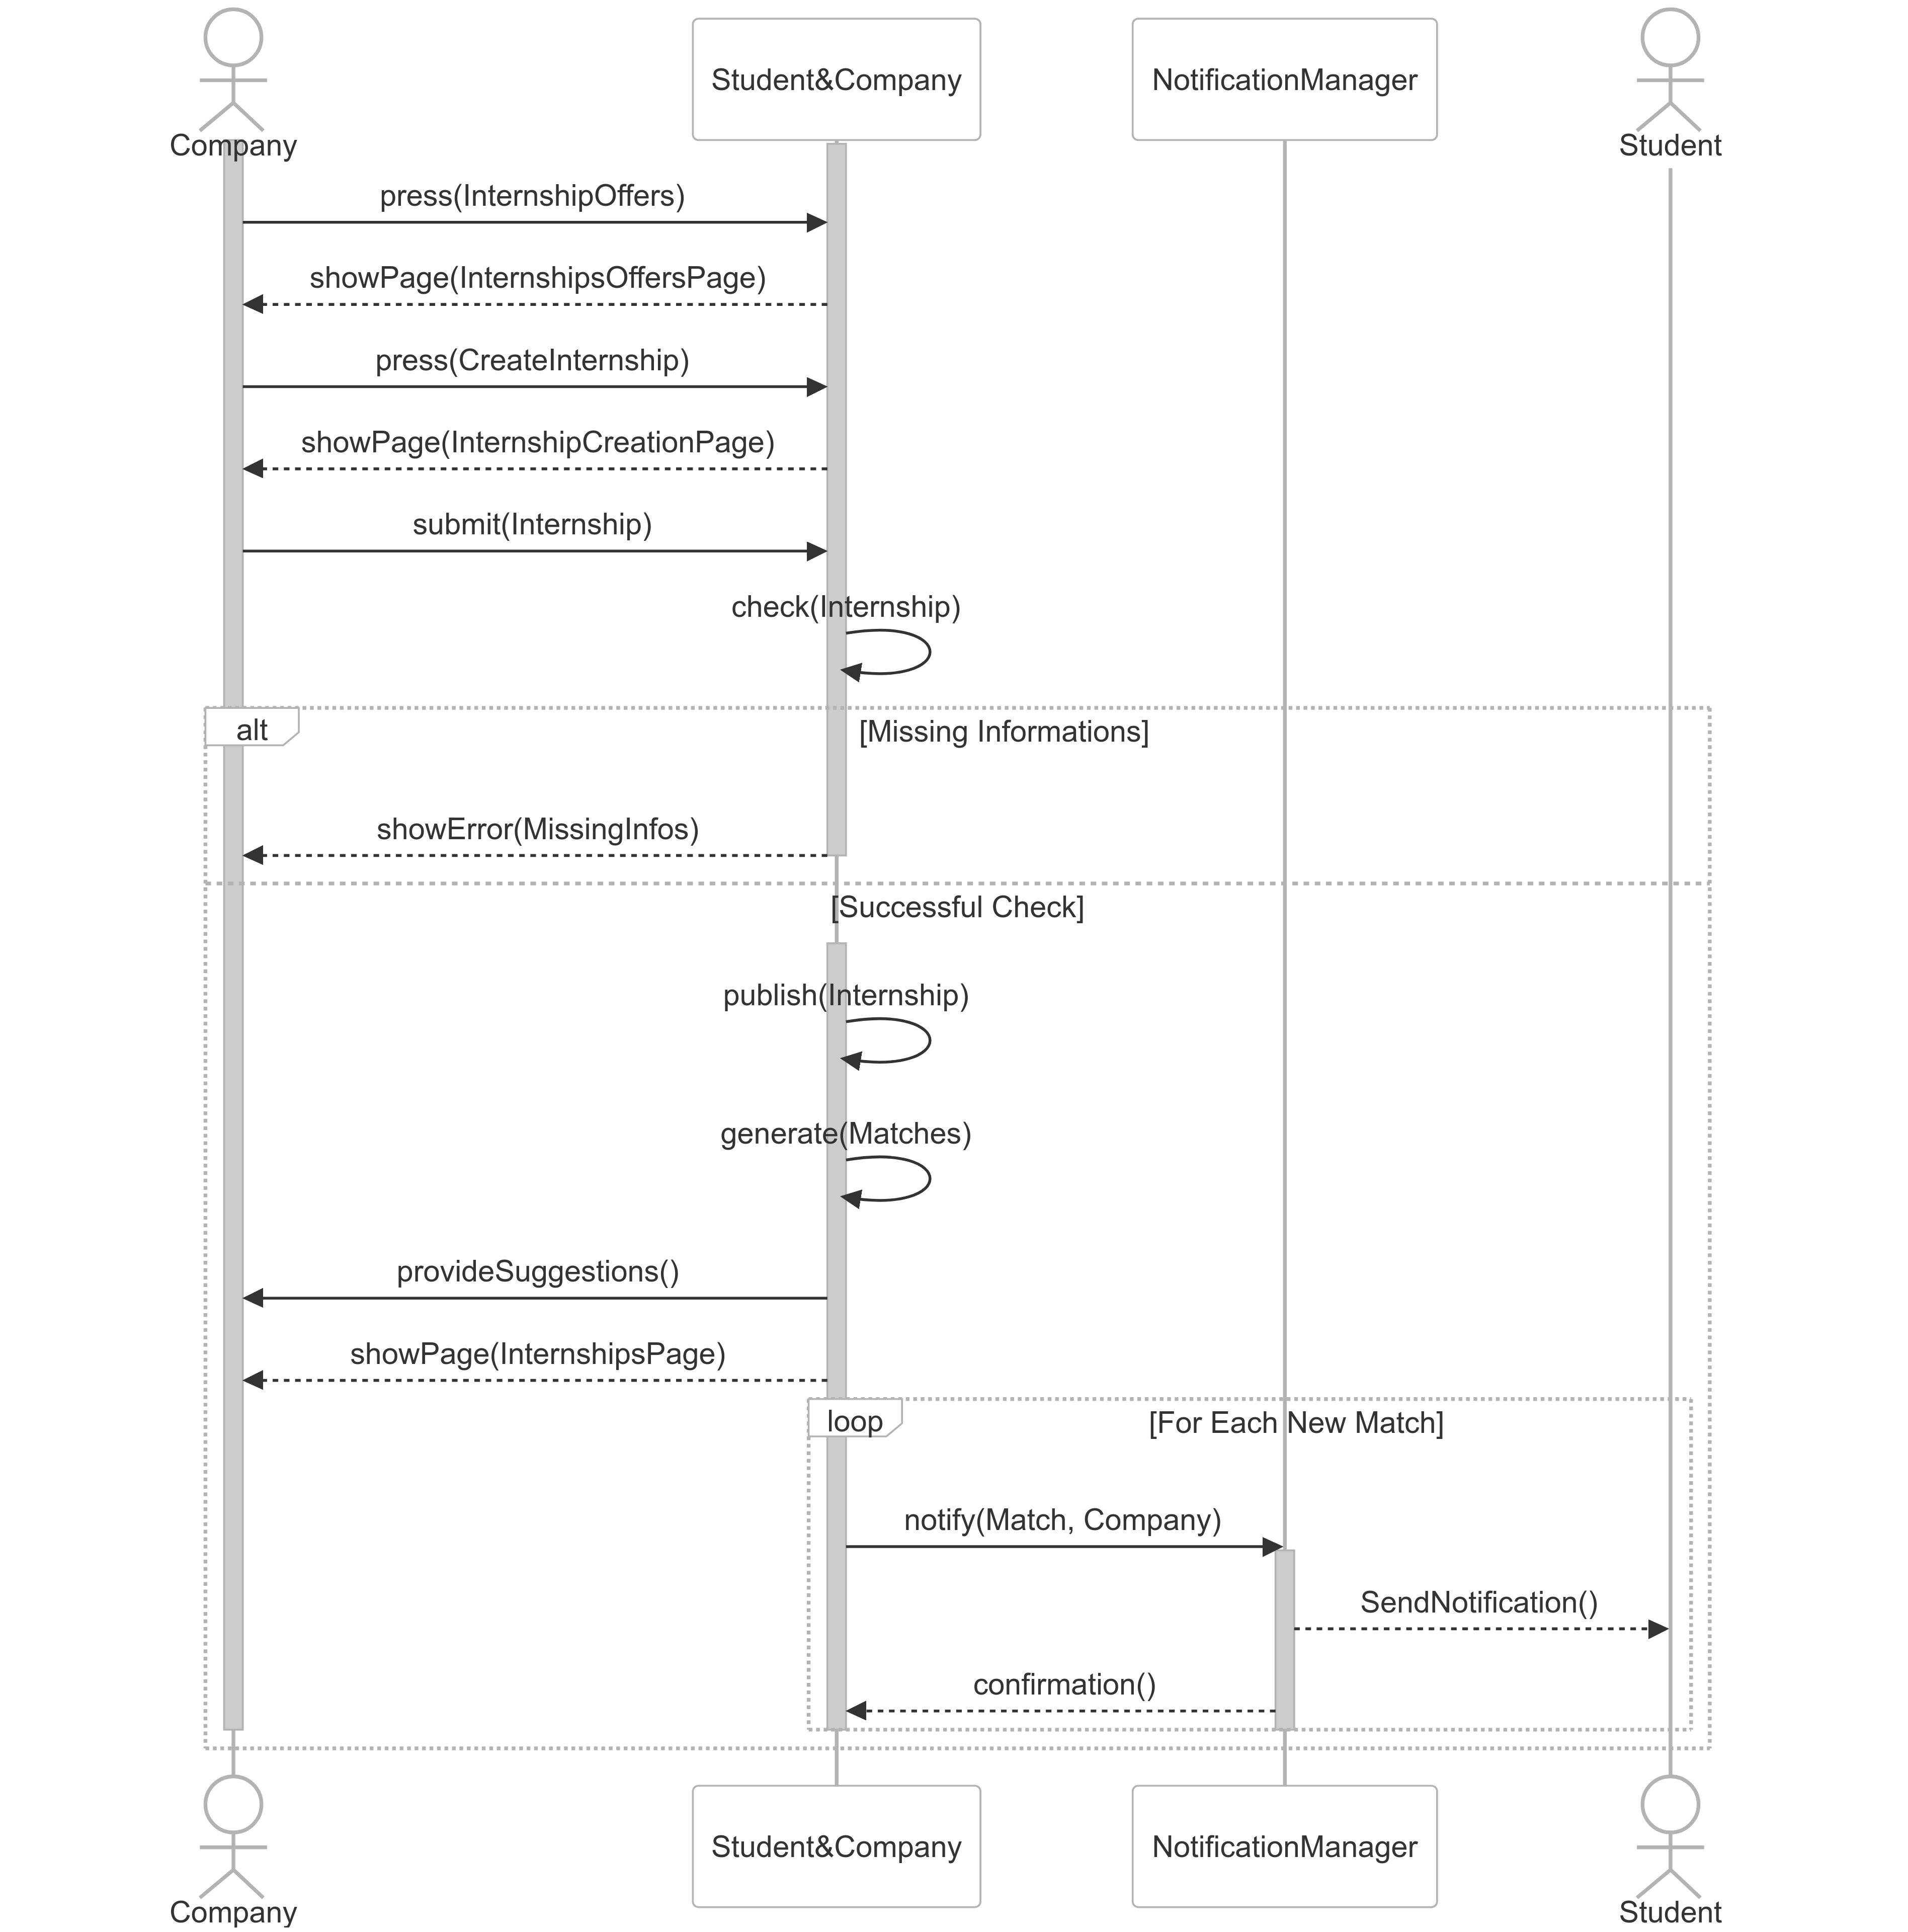
\includegraphics[width=0.8\textwidth]{Latex/Images/RASD/SequenceDiagrams/AdvertiseInternshipSequenceDiagram.png}
    \caption{[SD6]: Advertise Internship Sequence Diagram}
    \label{fig:SD6}
\end{figure}
\clearpage

\begin{figure}
    \centering
    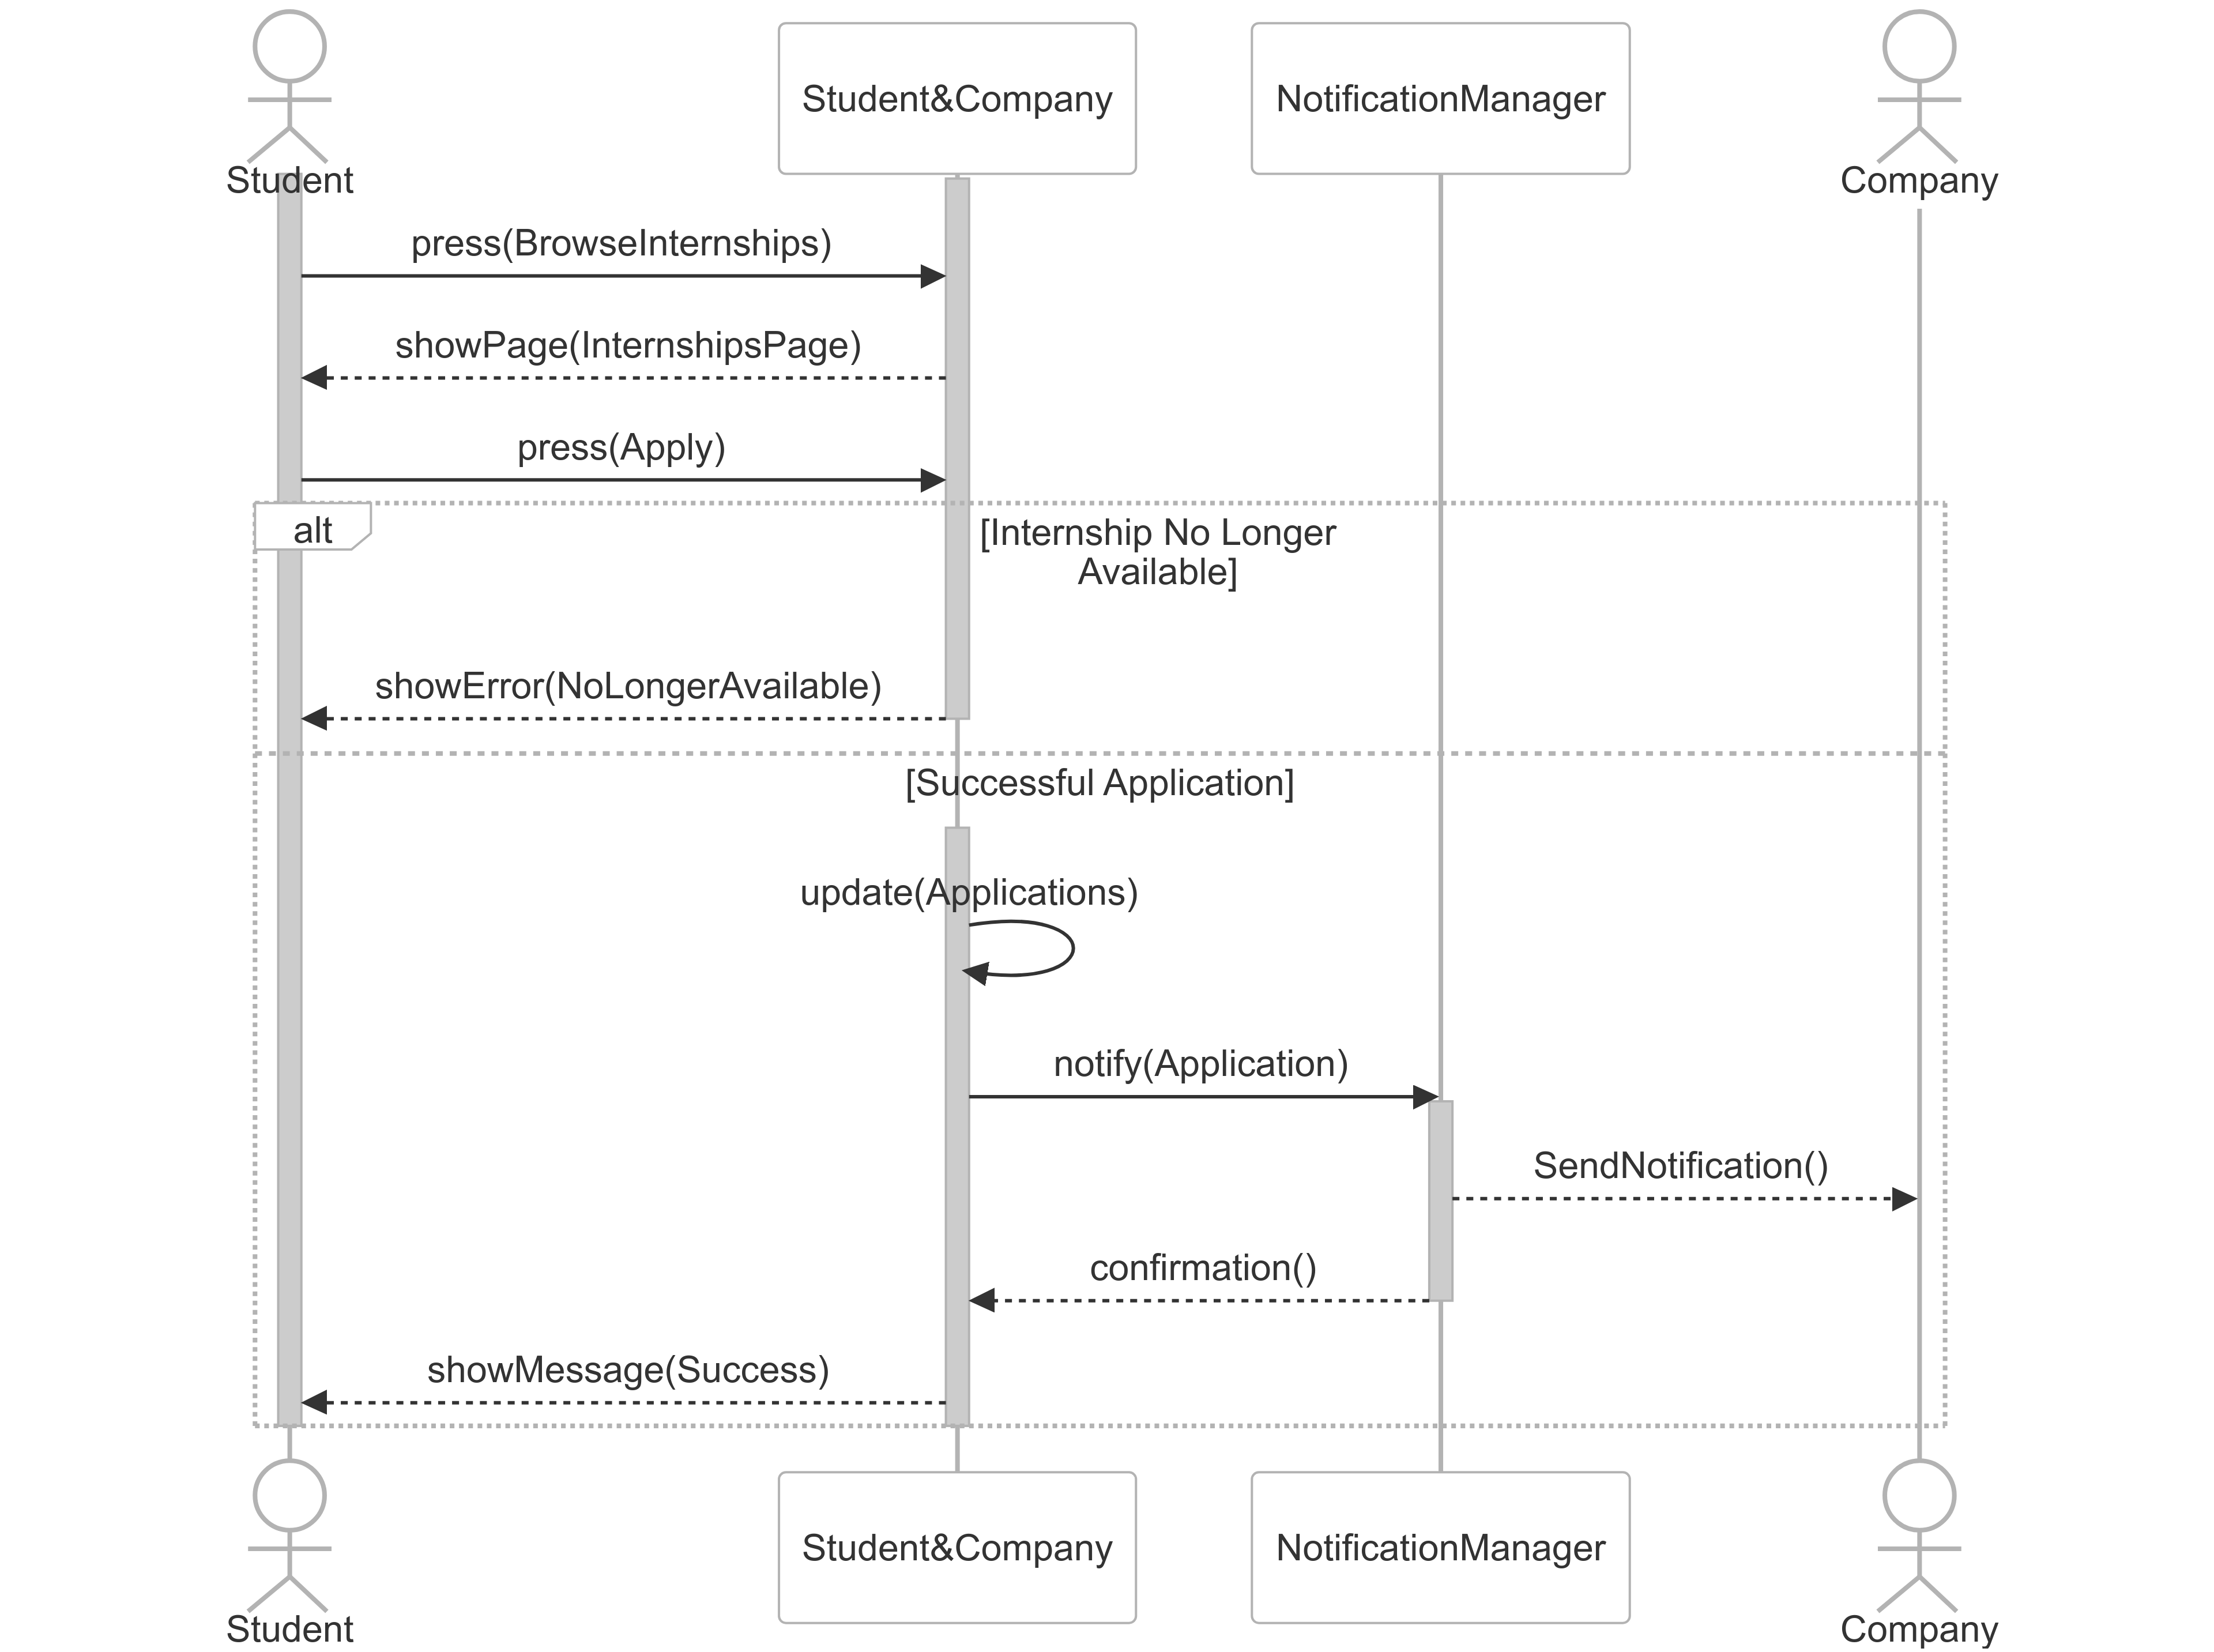
\includegraphics[width=0.8\textwidth]{Latex/Images/RASD/SequenceDiagrams/SpontaneousApplicationSequenceDiagram.png}
    \caption{[SD7]: Spontaneous Application Sequence Diagram}
    \label{fig:SD7}
\end{figure}

\begin{figure}
    \centering
    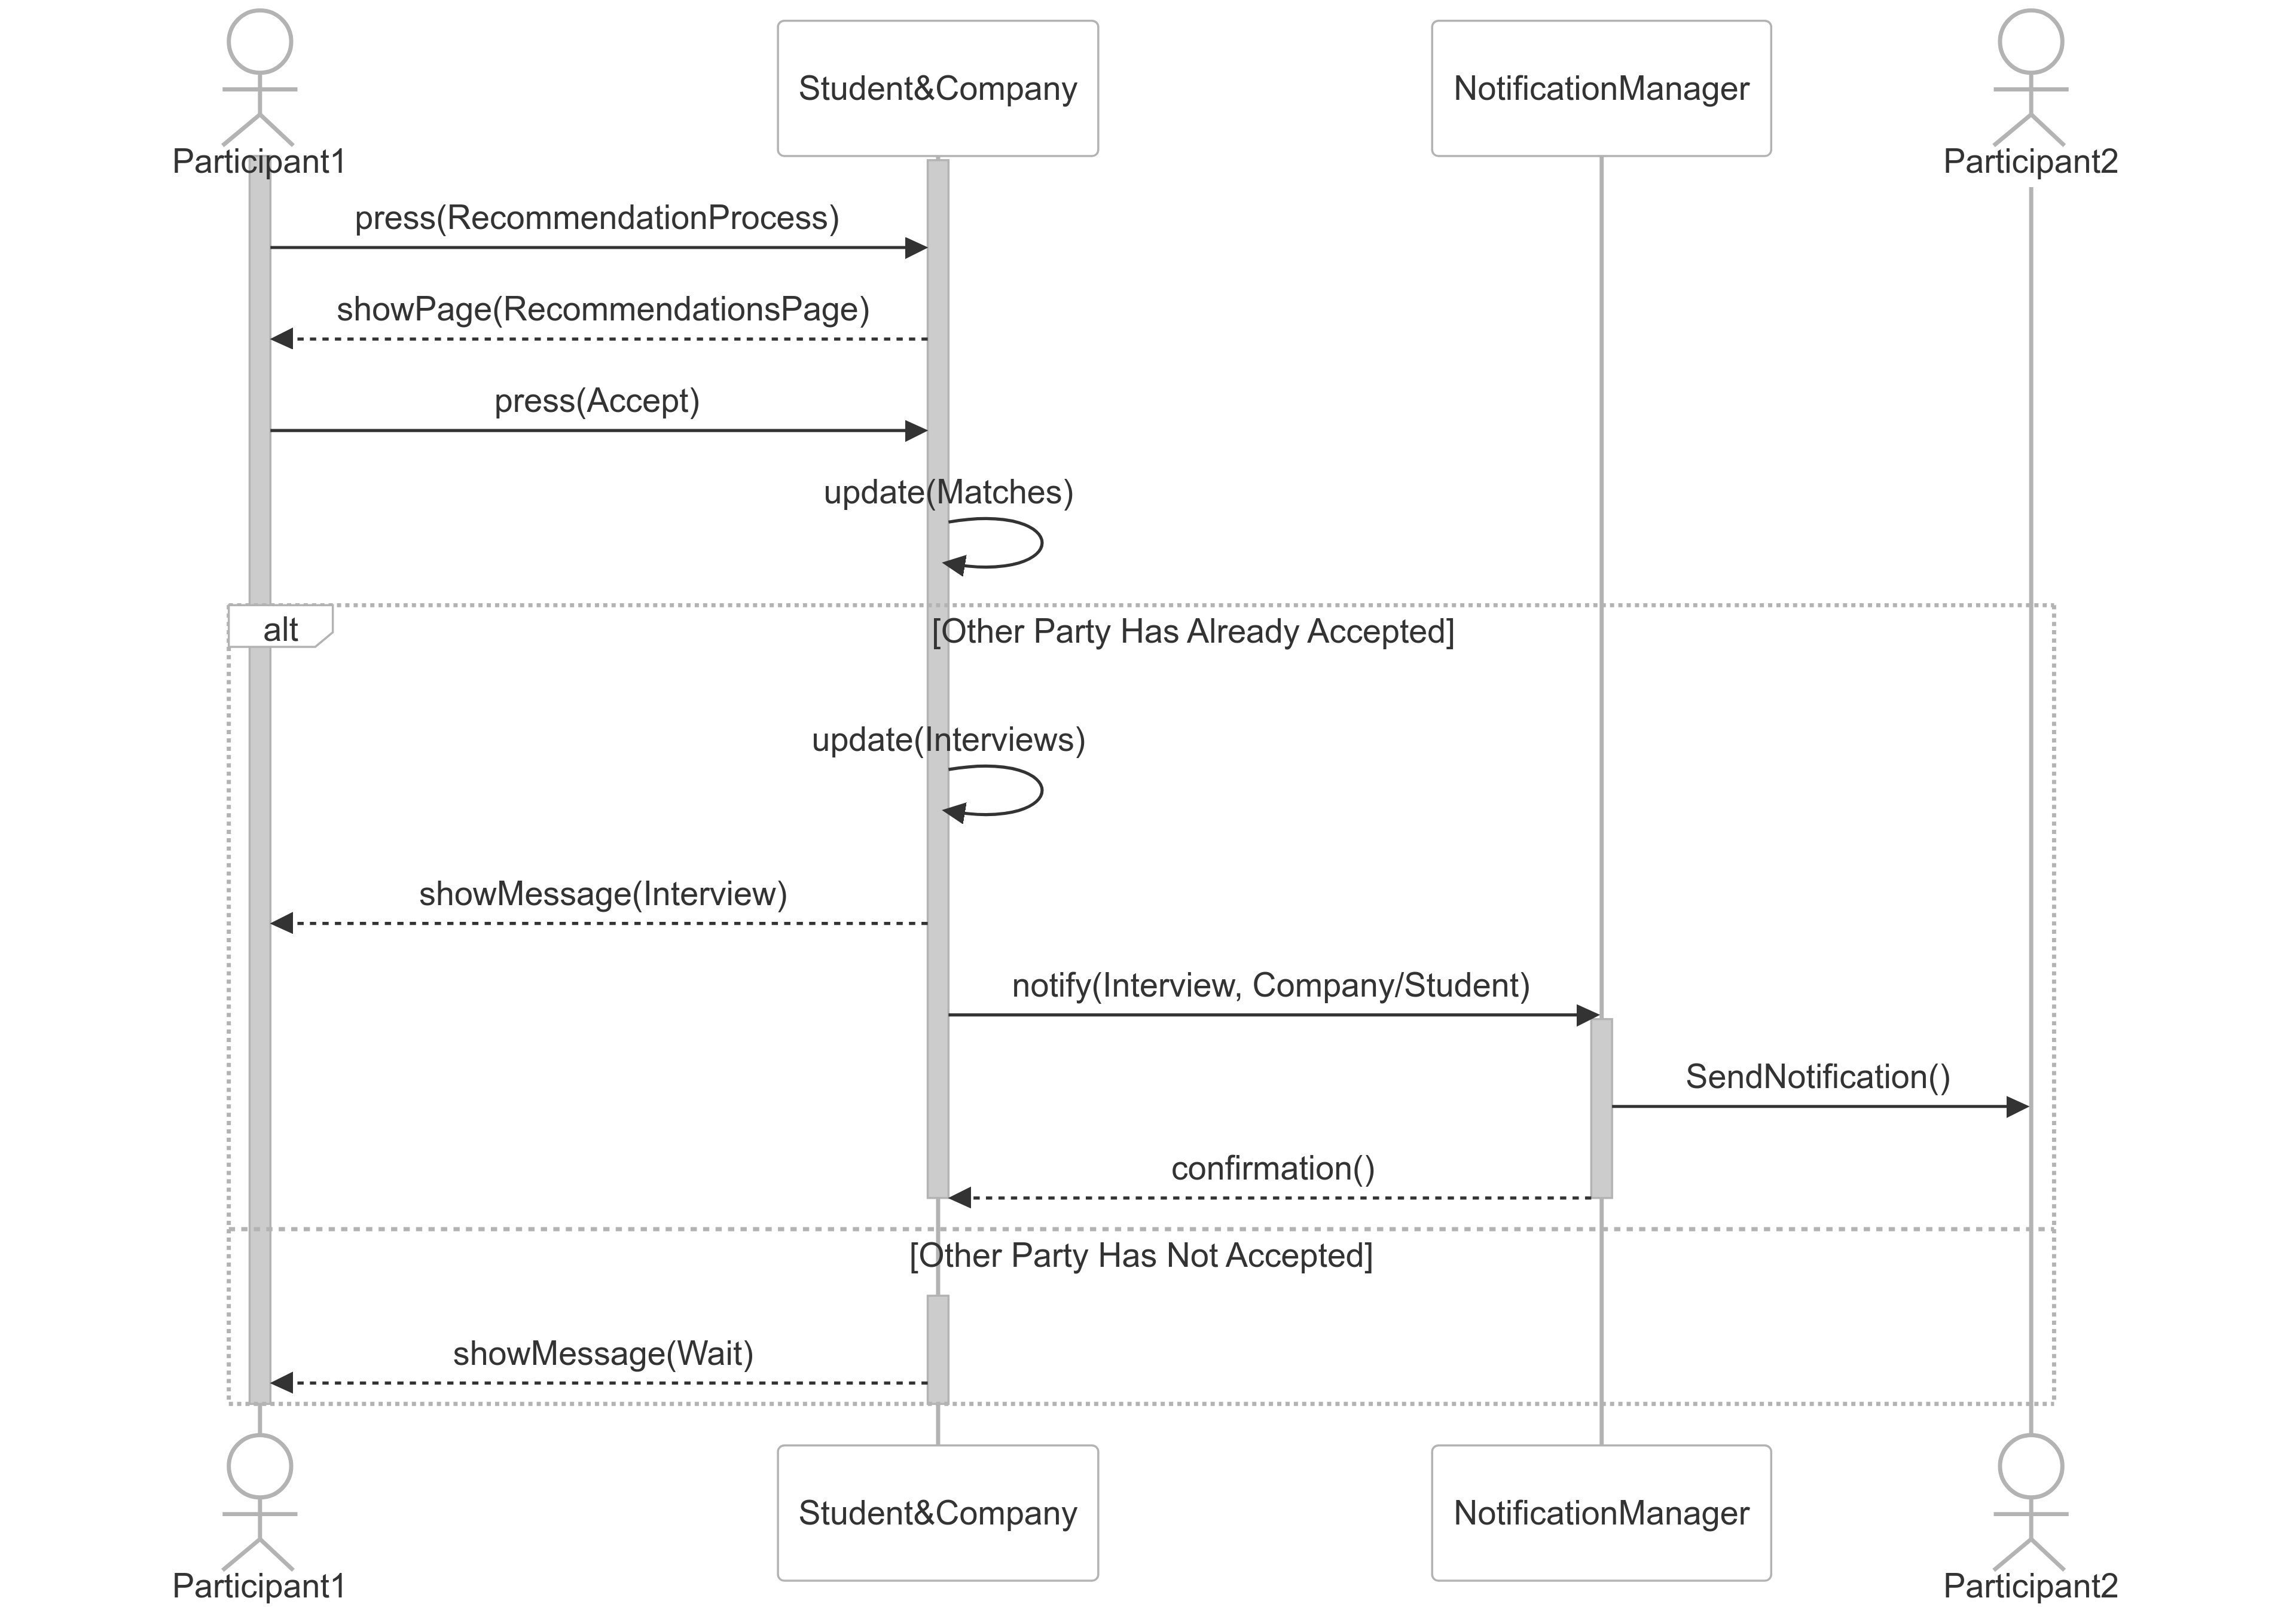
\includegraphics[width=0.8\textwidth]{Latex/Images/RASD/SequenceDiagrams/AcceptMatchSequenceDiagram.png}
    \caption{[SD8]: Accept Match Sequence Diagram}
    \label{fig:SD8}
\end{figure}
\clearpage

\begin{figure}
    \centering
    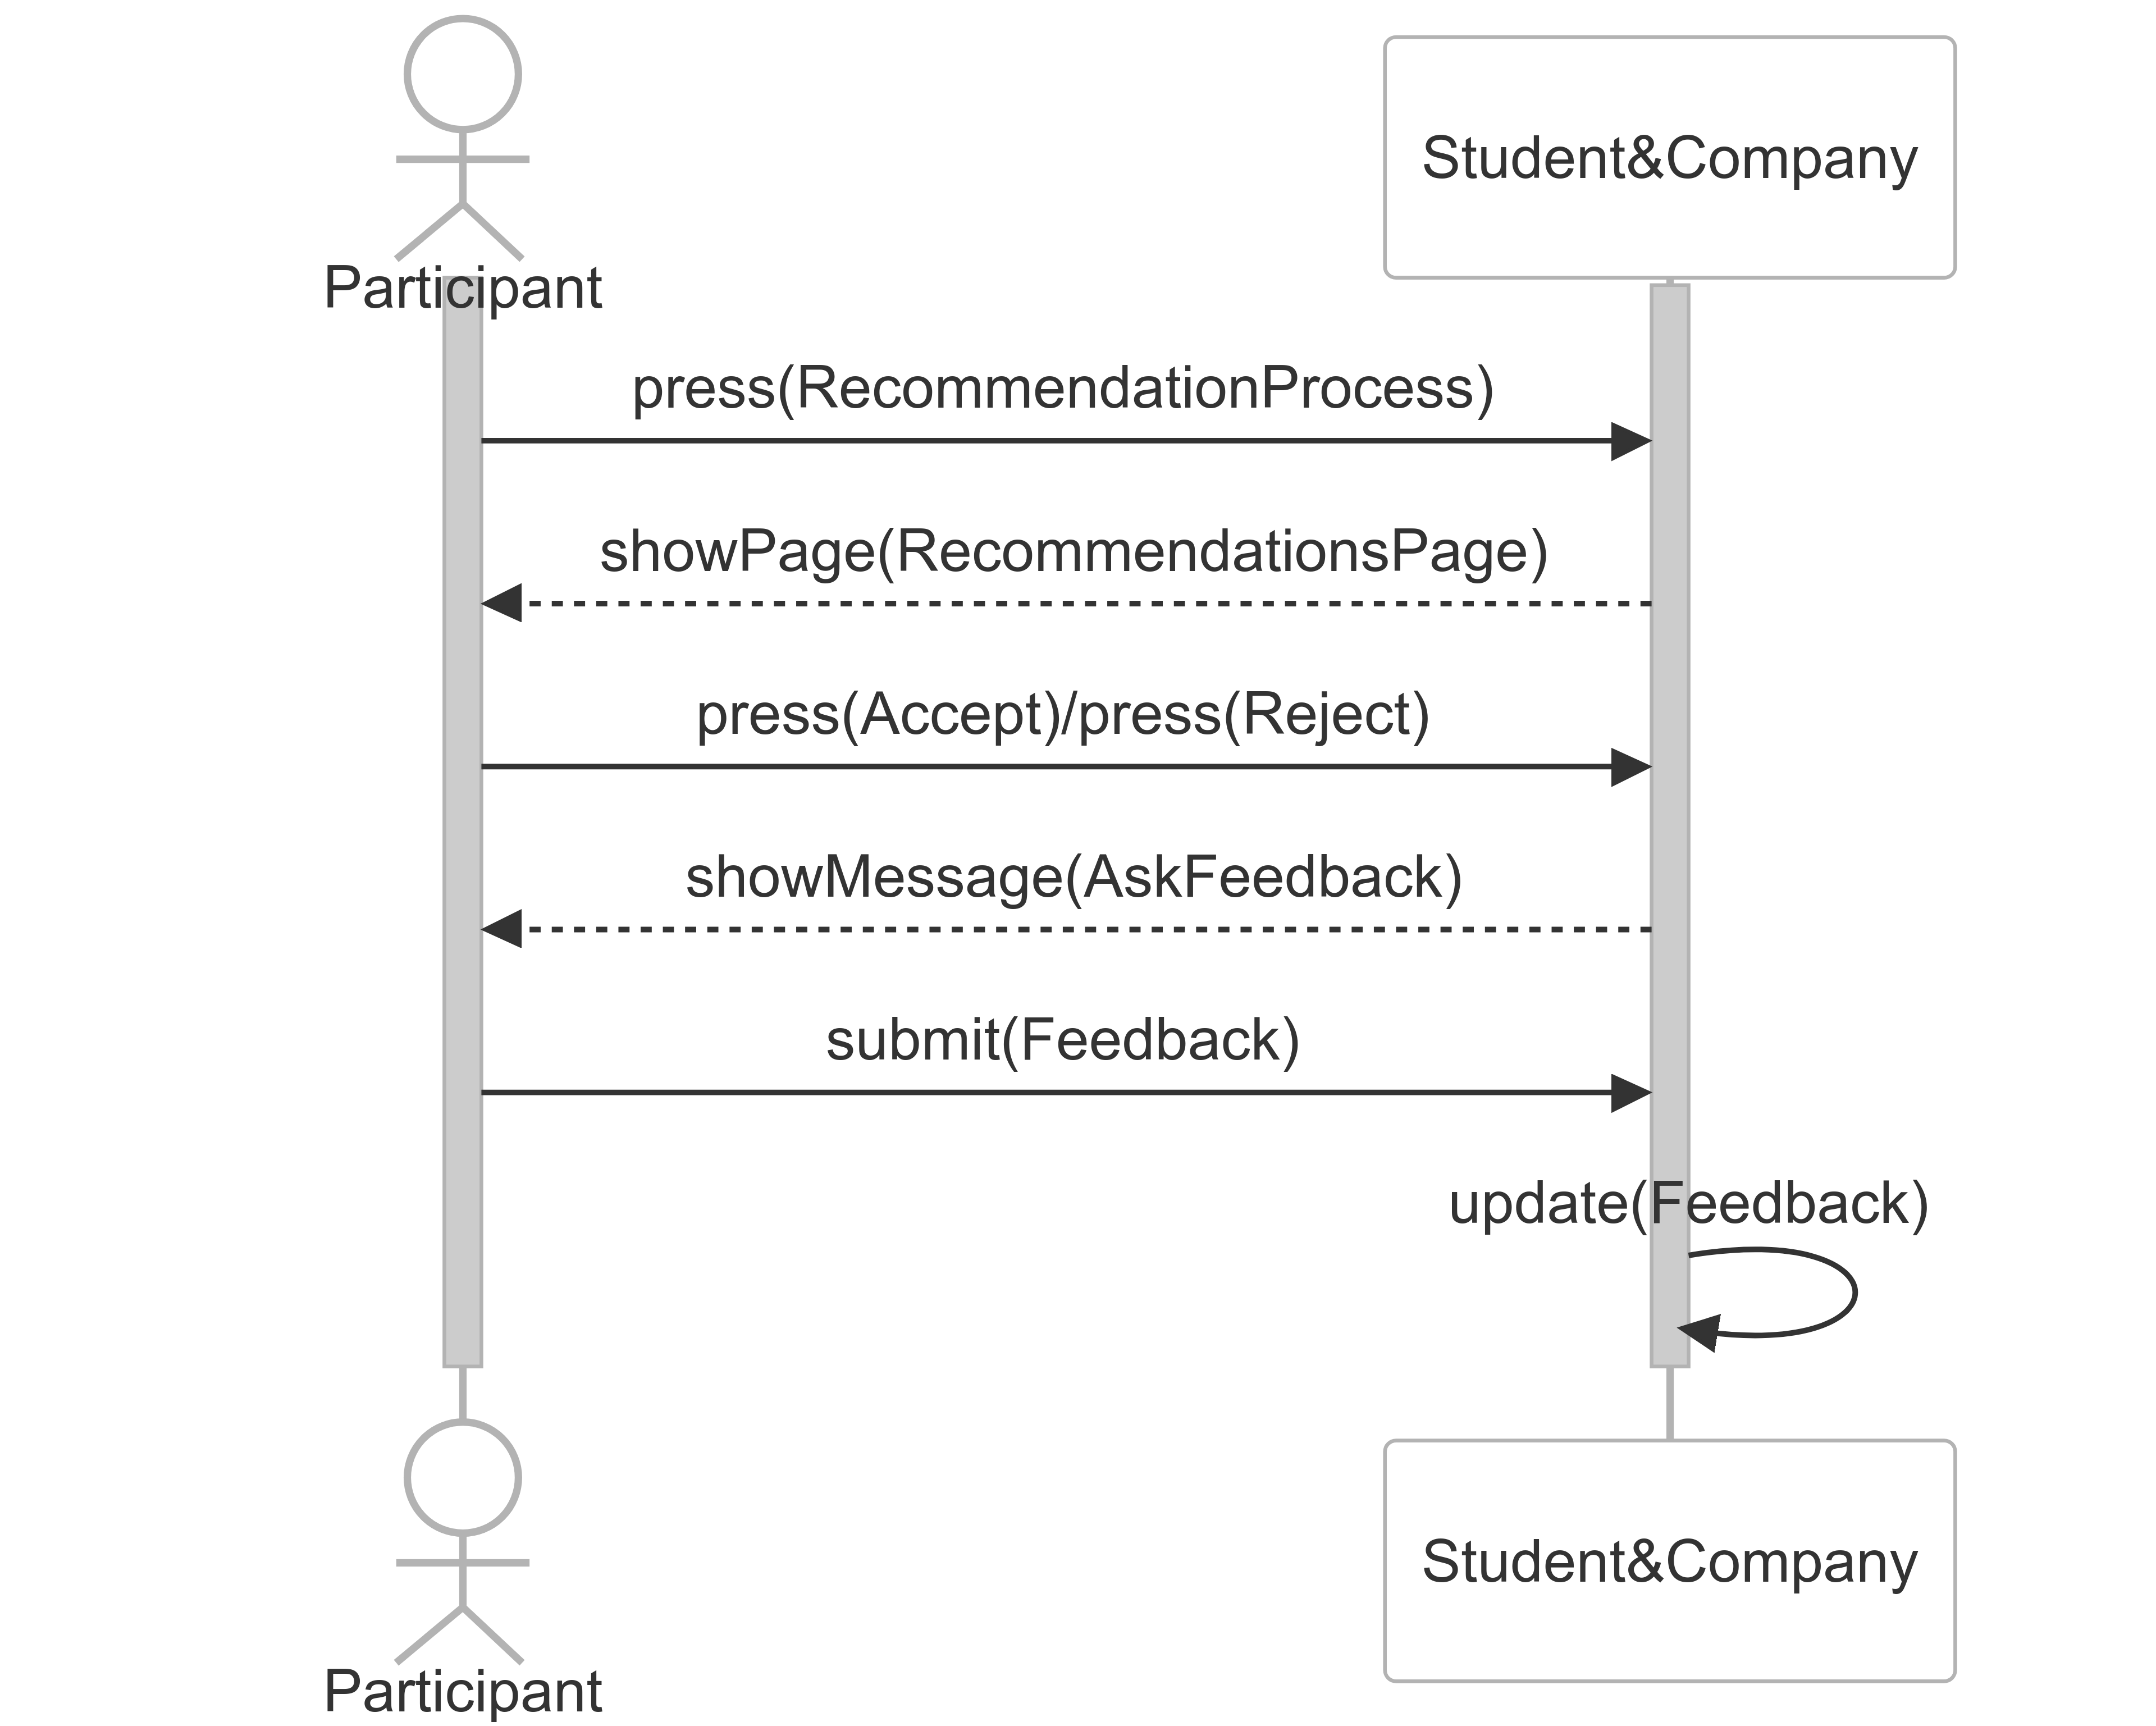
\includegraphics[width=0.55\textwidth]{Latex/Images/RASD/SequenceDiagrams/FeedbackMechanismSequenceDiagram.png}
    \caption{[SD9]: Feedback mechanism Sequence Diagram}
    \label{fig:SD9}
\end{figure}

\begin{figure}
    \centering
    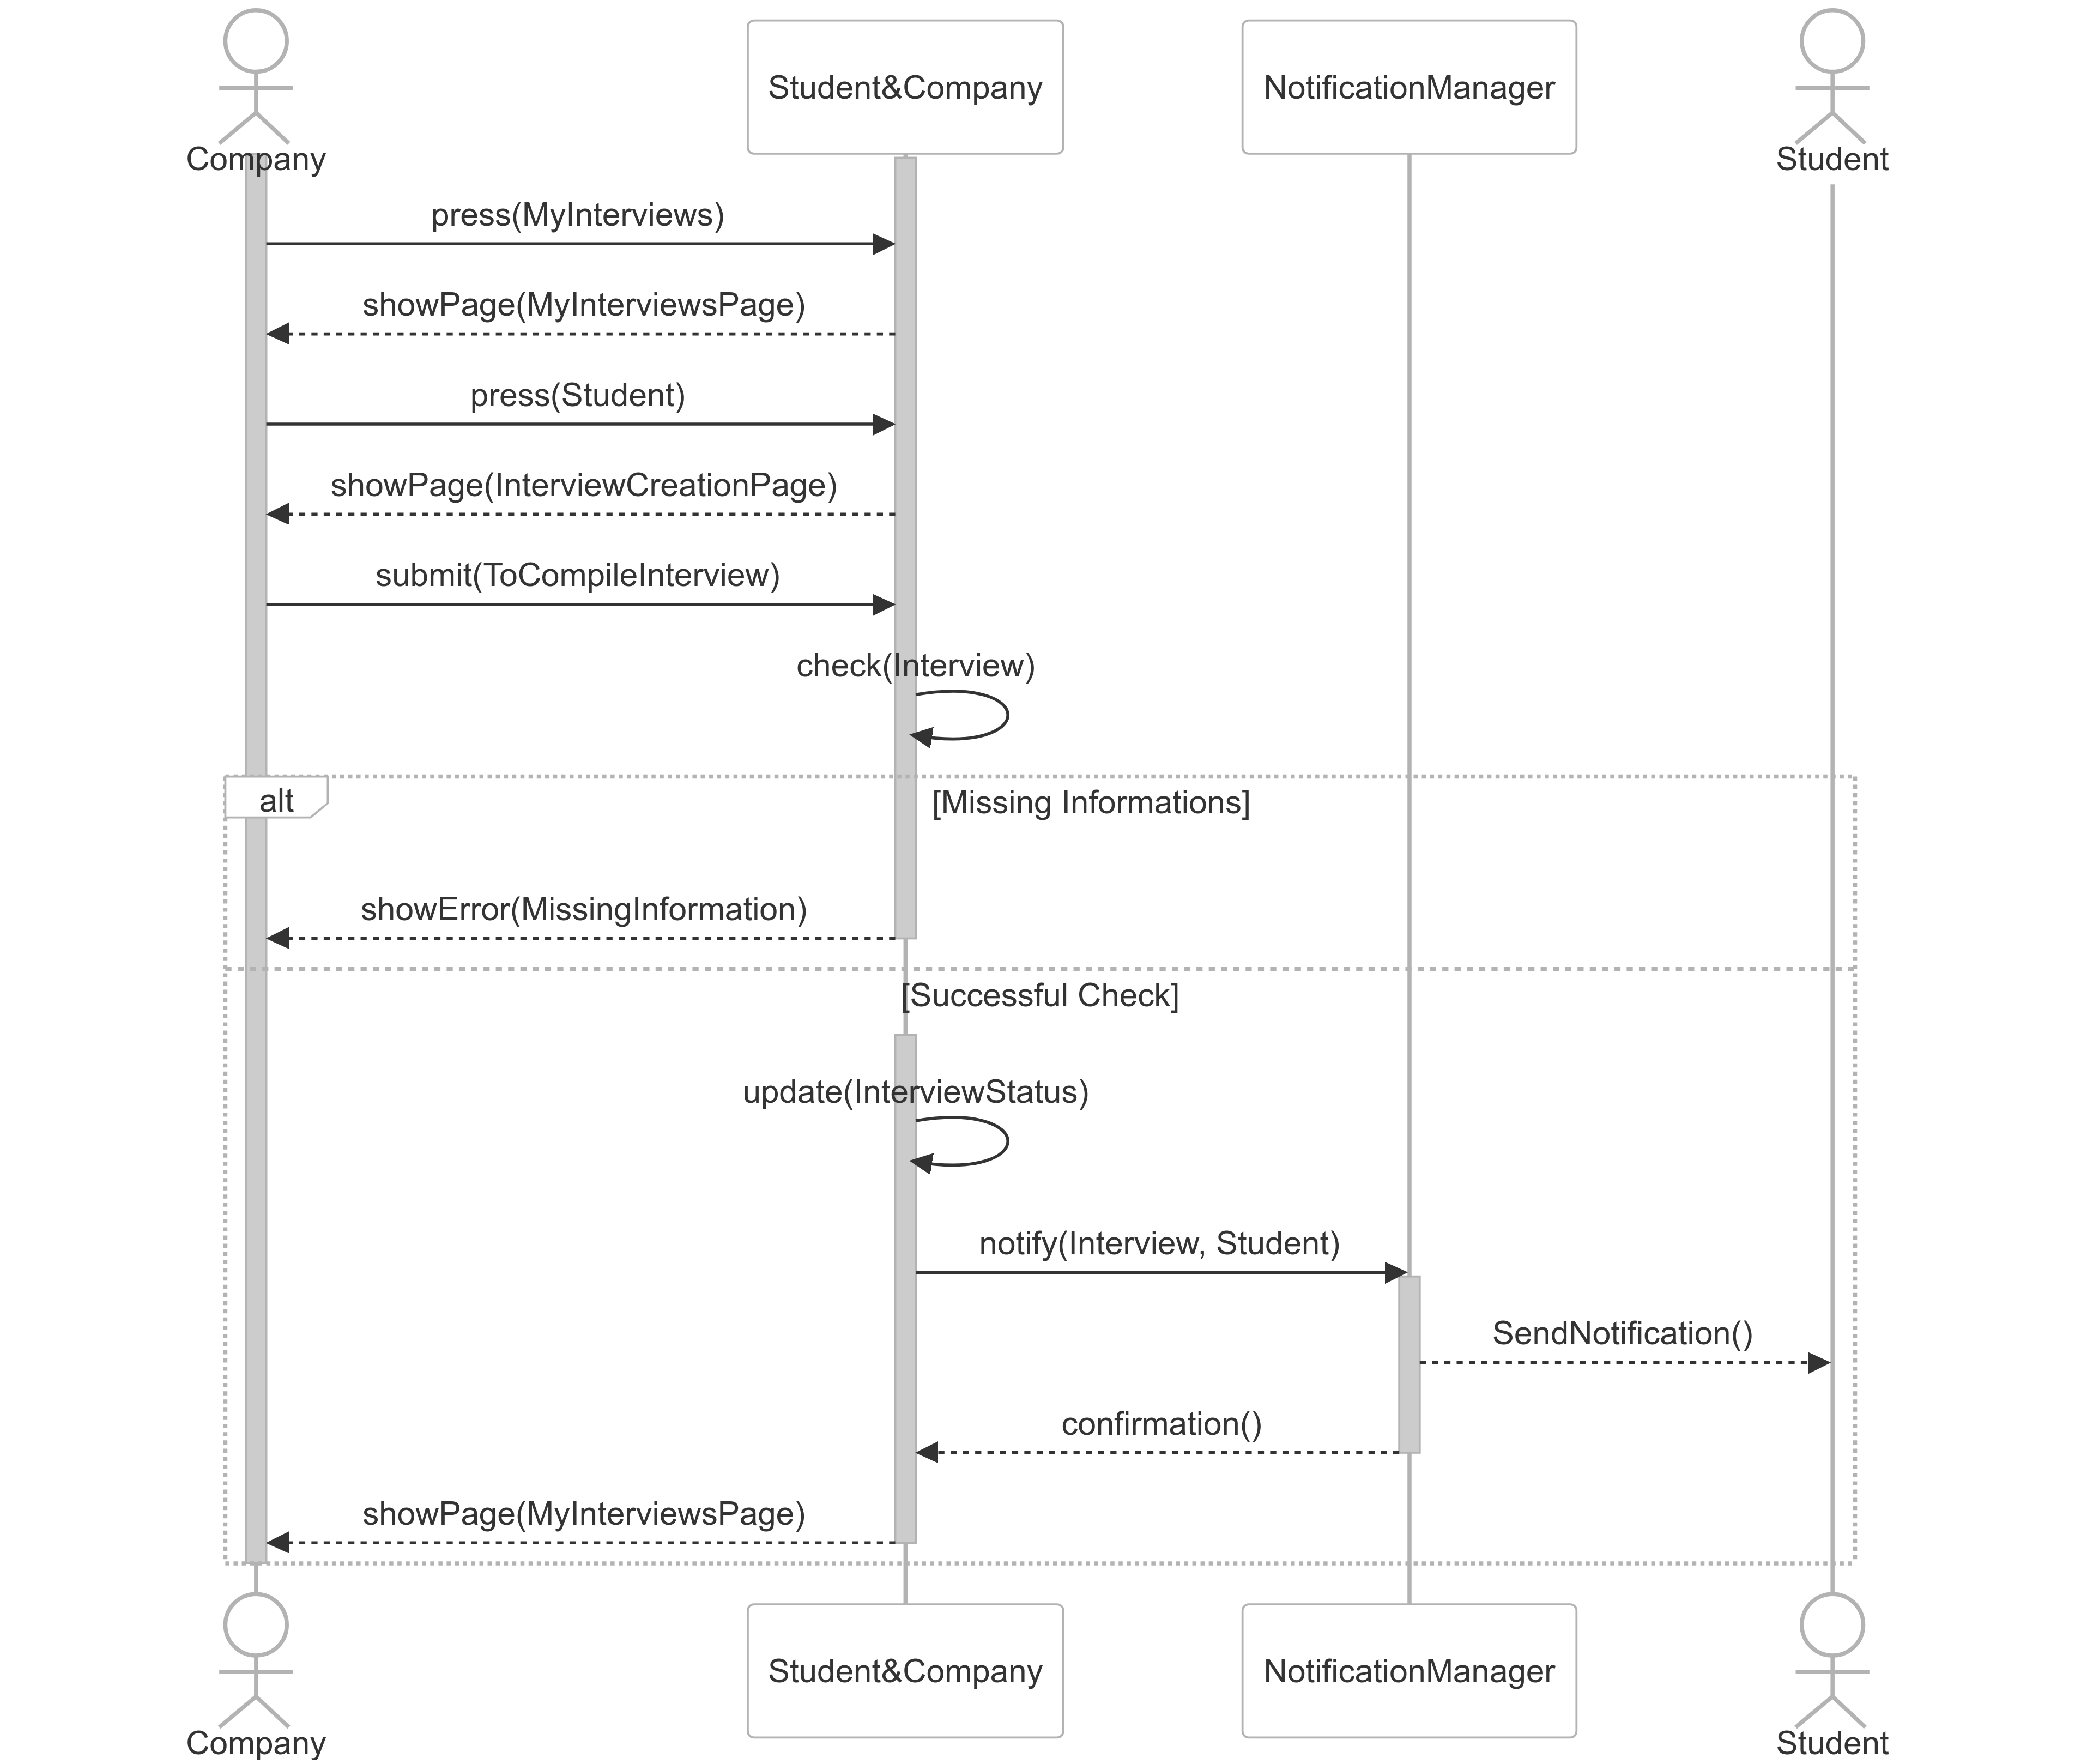
\includegraphics[width=0.8\textwidth]{Latex/Images/RASD/SequenceDiagrams/AssignInterviewSequenceDiagram.png}
    \caption{[SD10]: Assign Interview Sequence Diagram}
    \label{fig:SD10}
\end{figure}
\clearpage

\begin{figure}
    \centering
    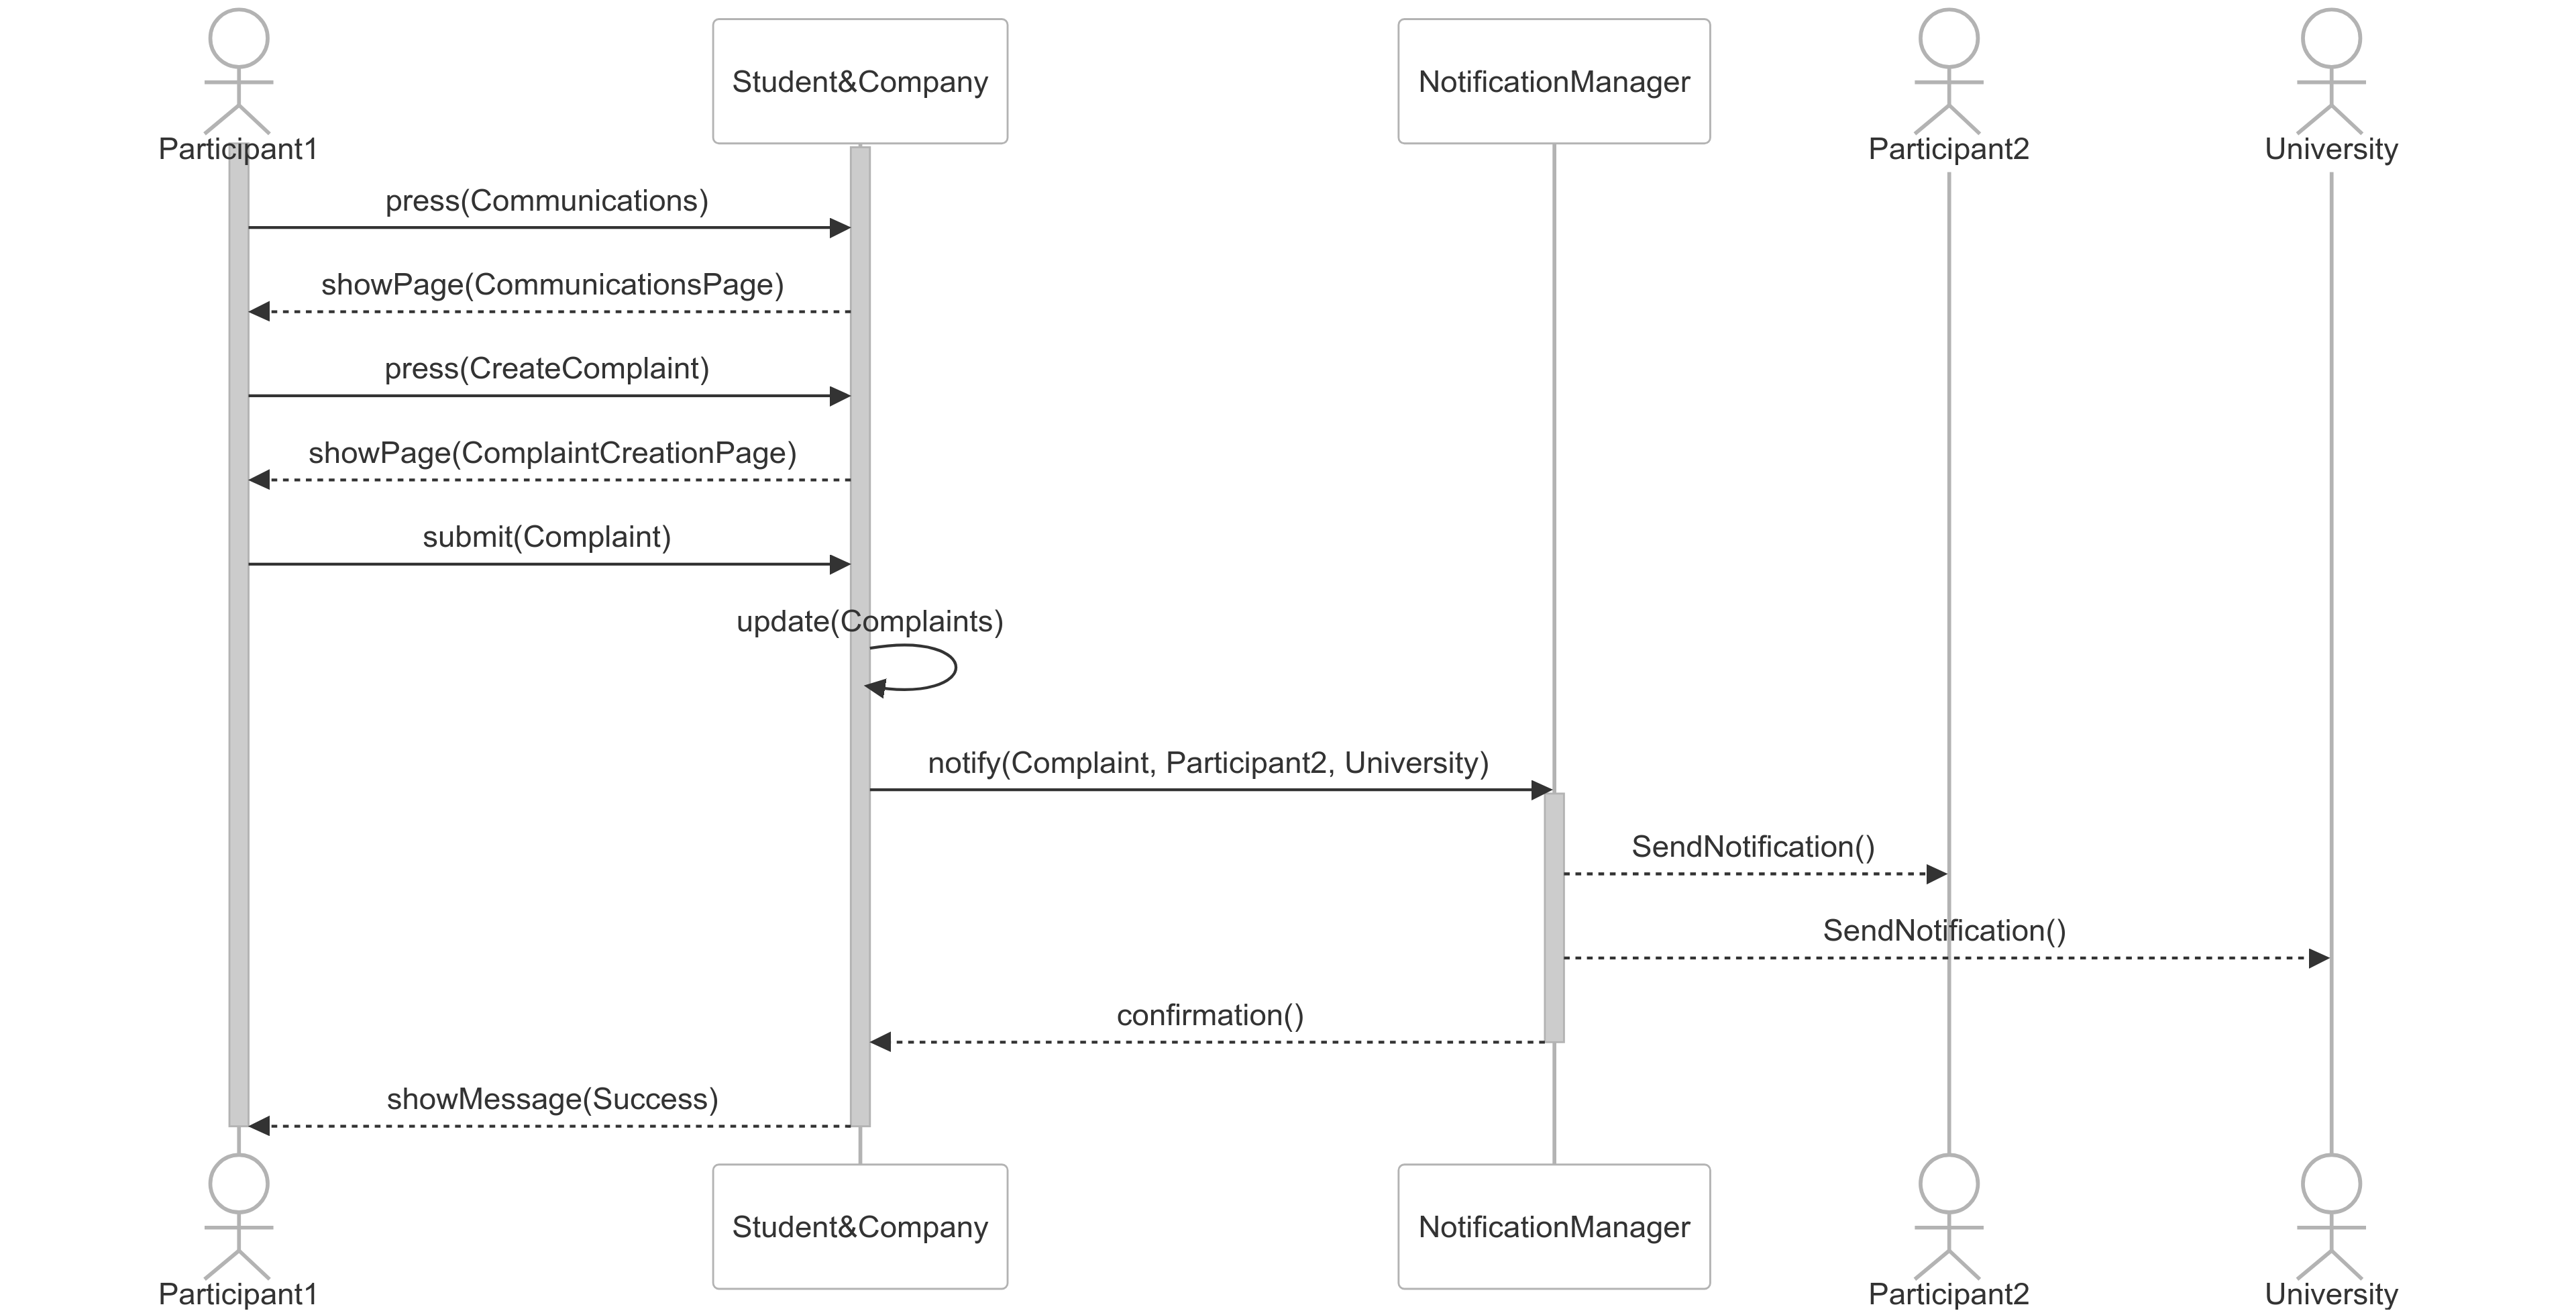
\includegraphics[width=1\textwidth]{Latex/Images/RASD/SequenceDiagrams/PublishComplaintSequenceDiagram.png}
    \caption{[SD11]: Publish Complaint Sequence Diagram}
    \label{fig:SD11}
\end{figure}

\begin{figure}
    \centering
    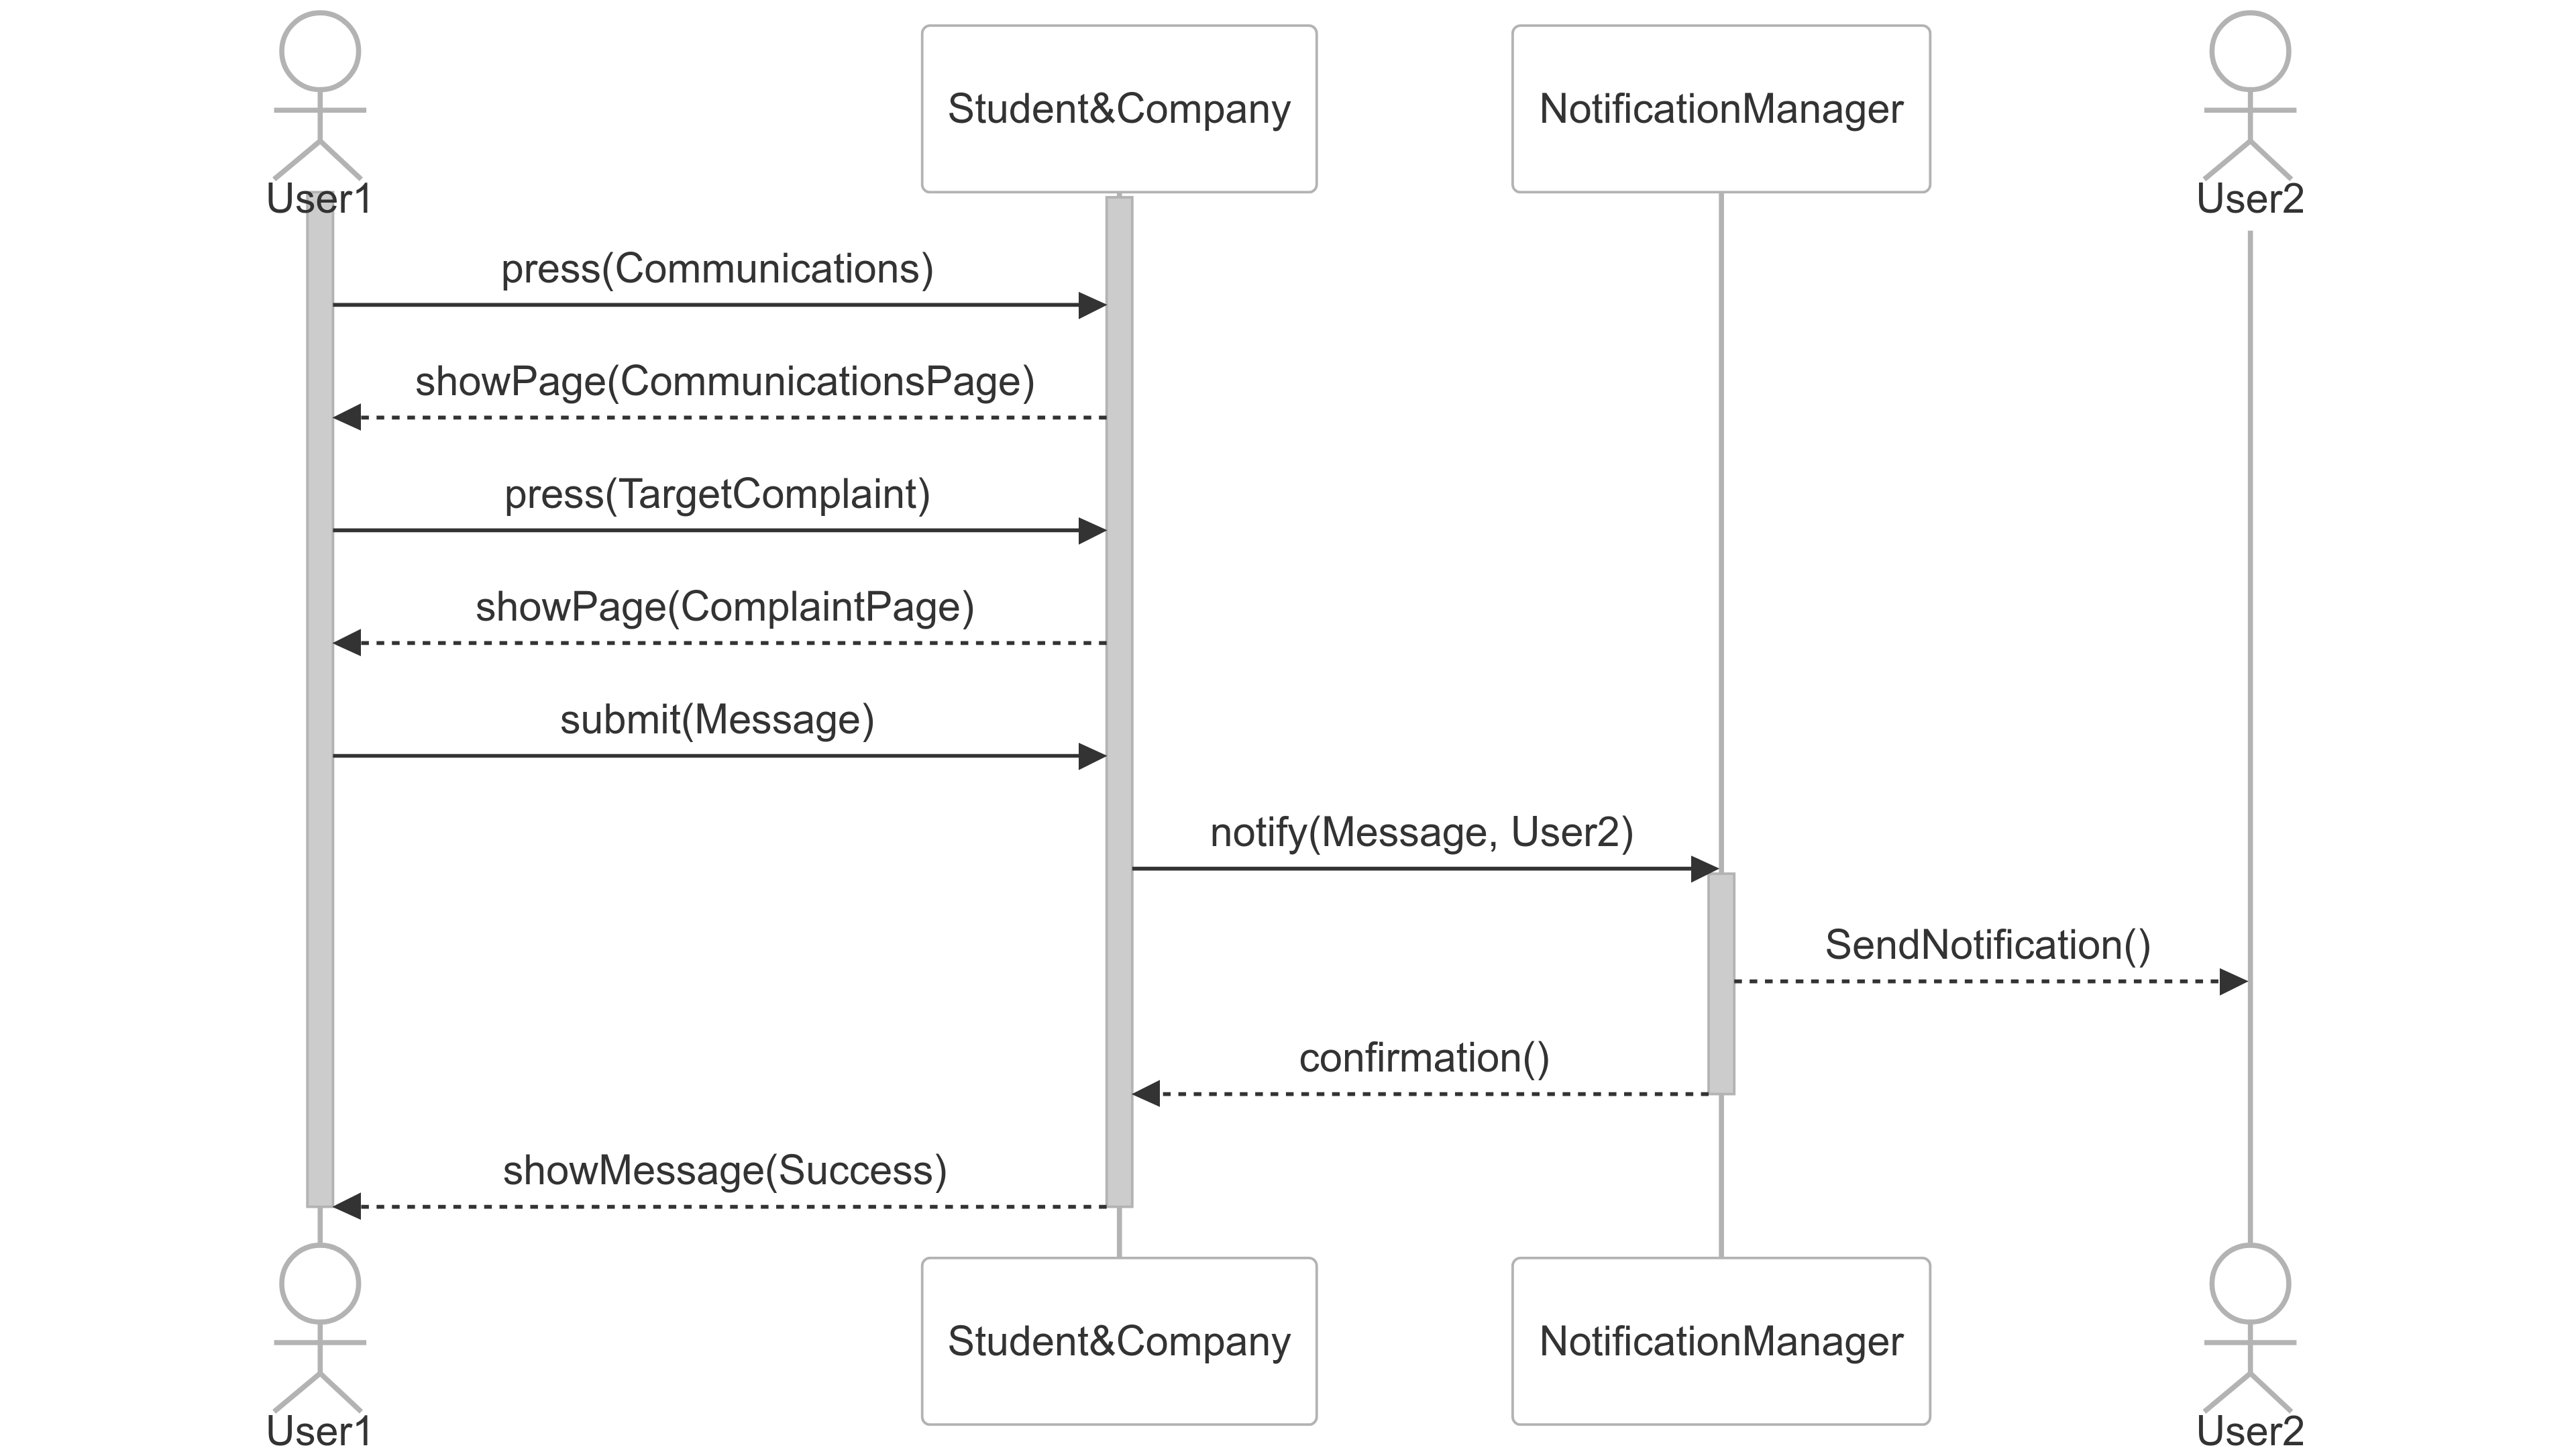
\includegraphics[width=0.7\textwidth]{Latex/Images/RASD/SequenceDiagrams/RespondToComplaintSequenceDiagram.png}
    \caption{[SD12]: Respond to Complaint Sequence Diagram}
    \label{fig:SD12}
\end{figure}

\begin{figure}
    \centering
    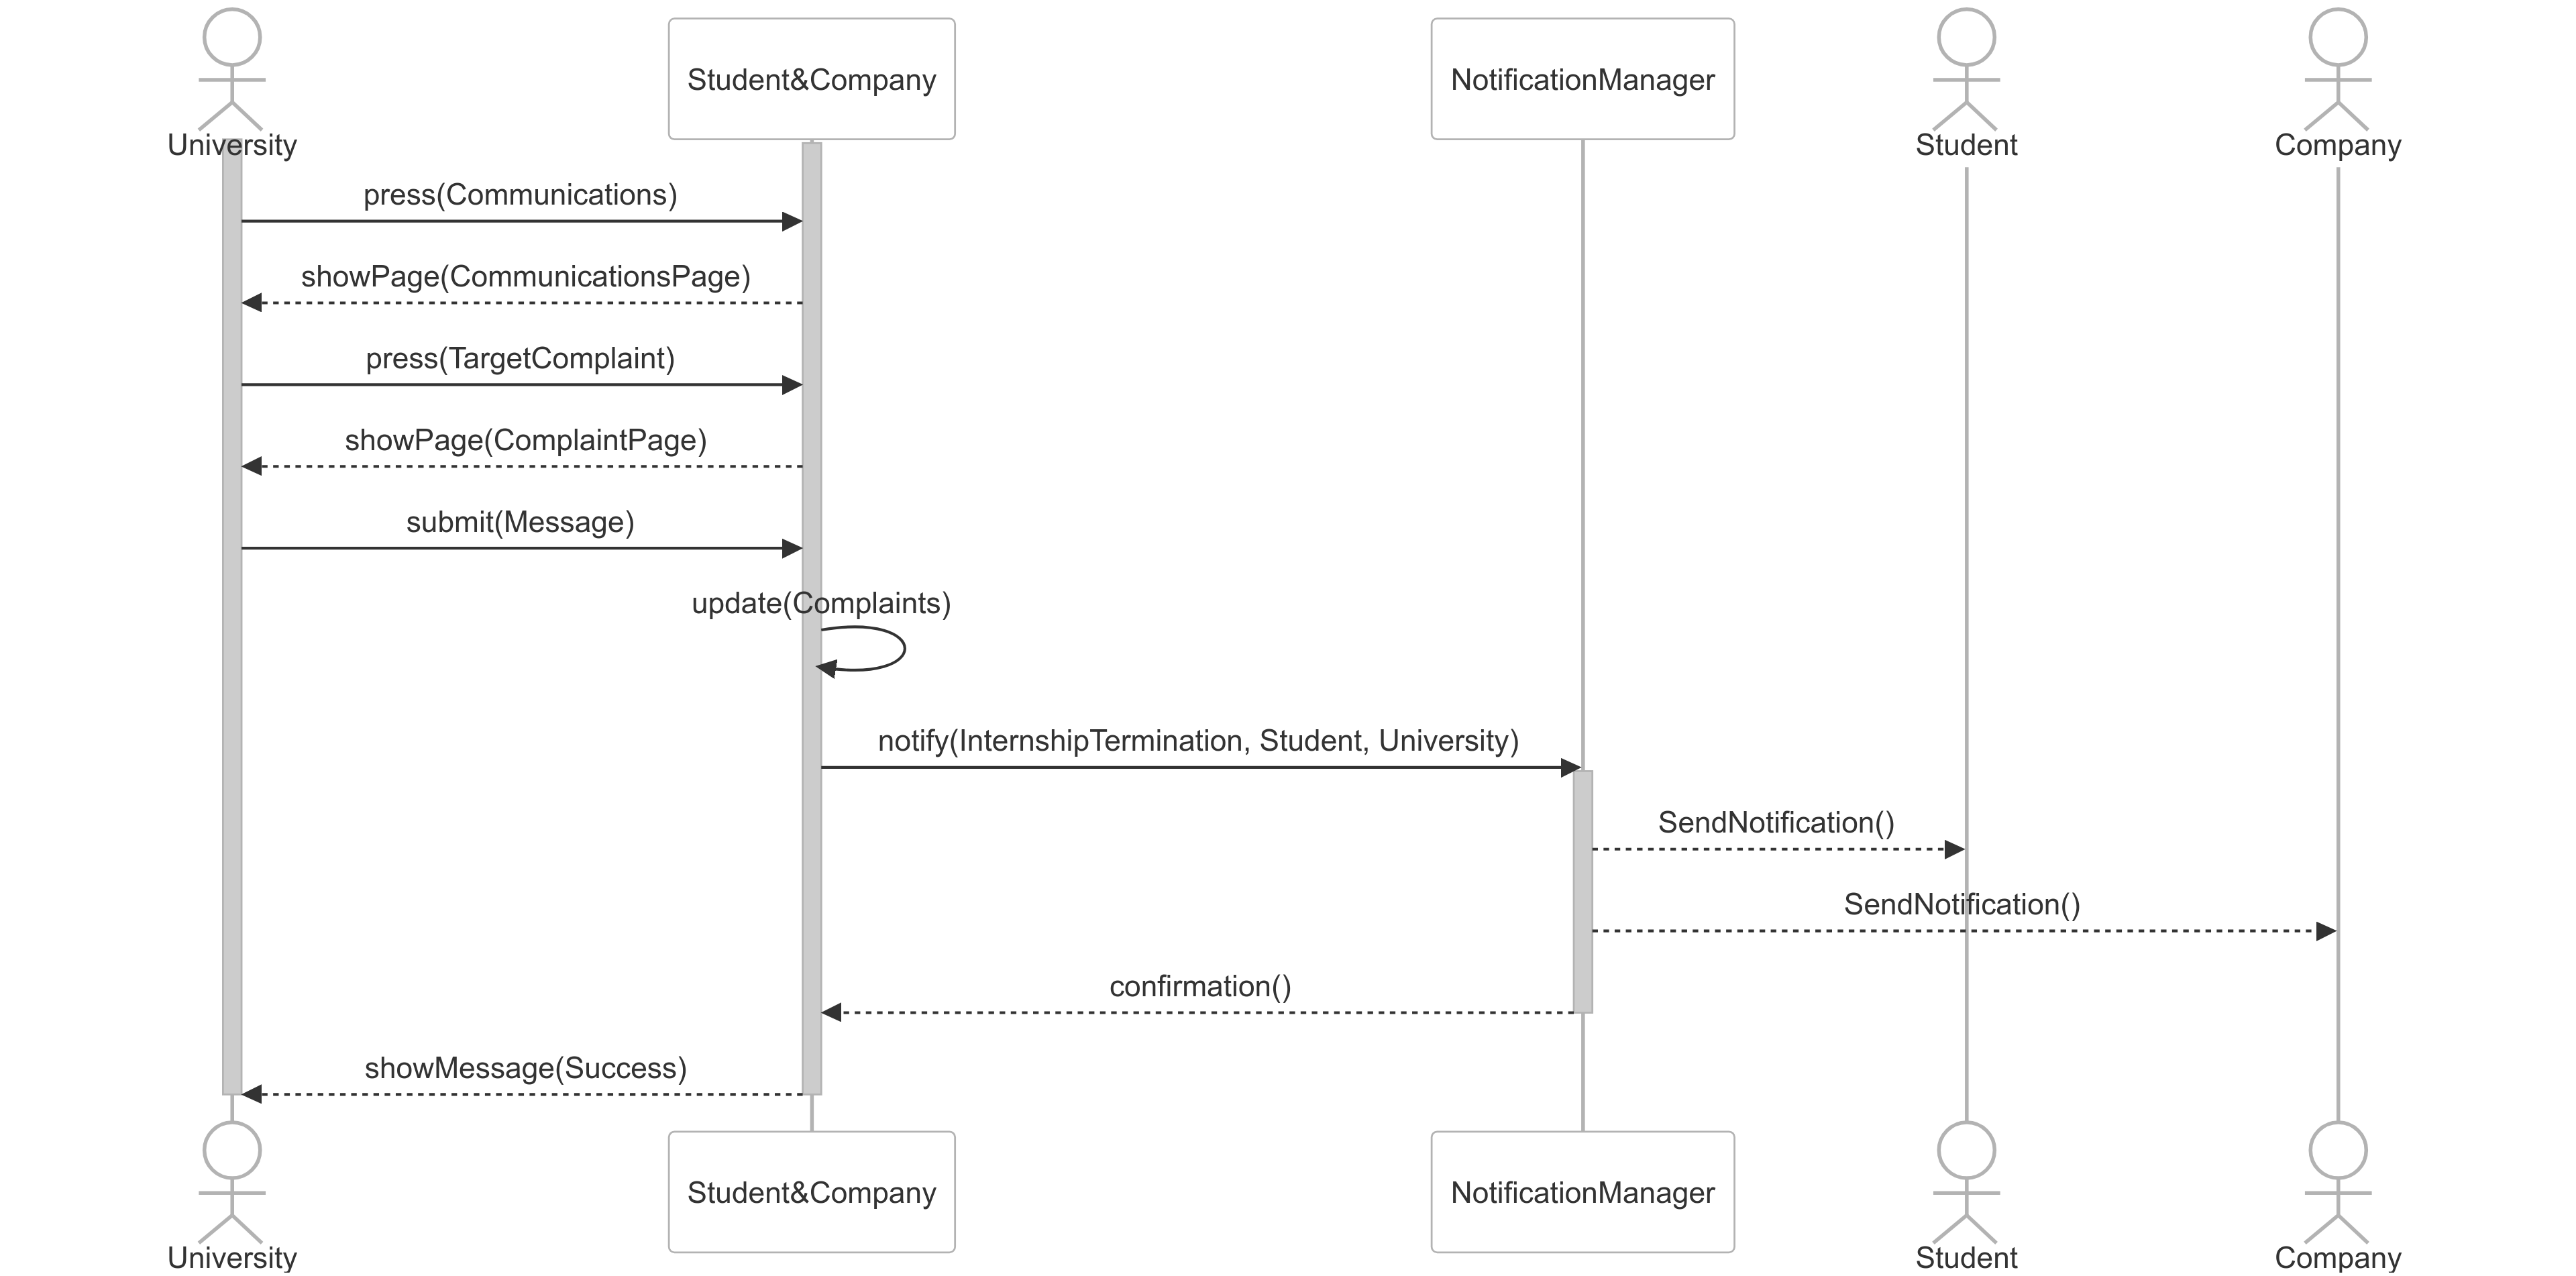
\includegraphics[width=1\textwidth]{Latex/Images/RASD/SequenceDiagrams/HandleComplaintSequenceDiagram.png}
    \caption{[SD13]: Handle Complaint Sequence Diagram}
    \label{fig:SD13}
\end{figure}

\begin{figure}
    \centering
    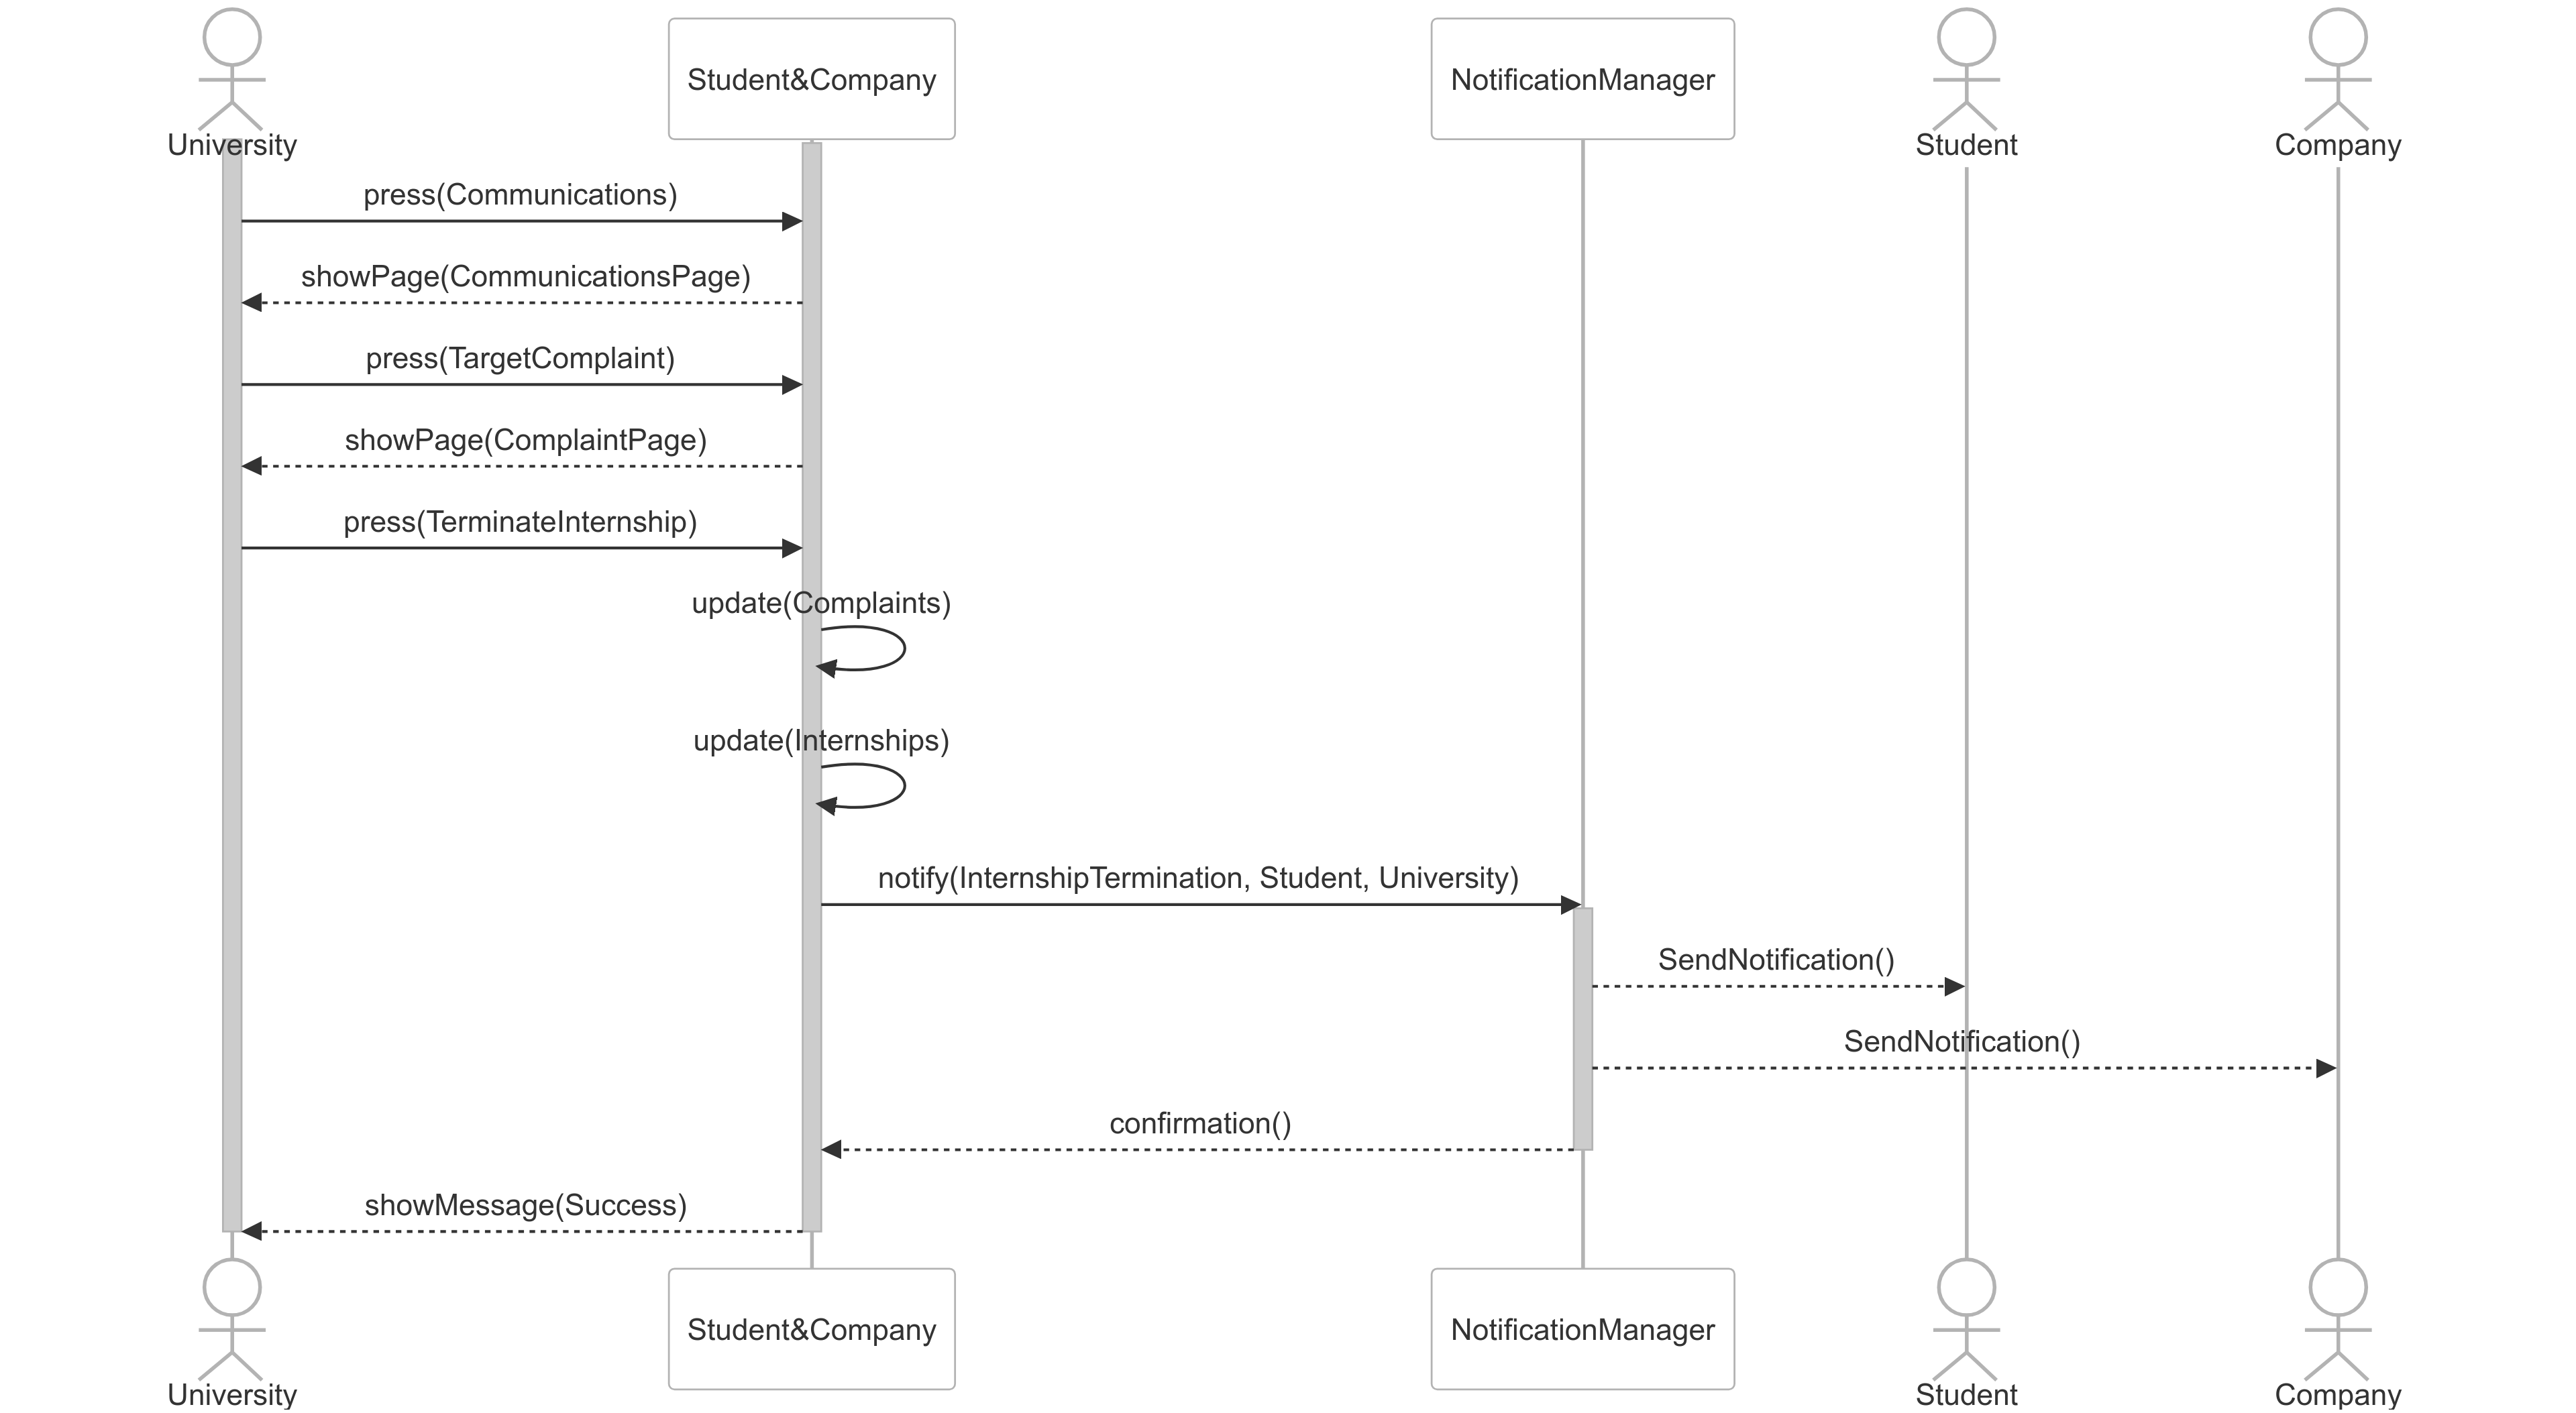
\includegraphics[width=1\textwidth]{Latex/Images/RASD/SequenceDiagrams/TerminateInternshipSequenceDiagram.png}
    \caption{[SD14]: Terminate Internship Sequence Diagram}
    \label{fig:SD14}
\end{figure}
\clearpage

\subsubsection{Requirements Mapping}

\begin{table}[H]
    \centering
    \begin{tabular}{|p{15cm}|}
         \hline
        \textbf{G1:} Companies would like to advertise the internships they offer. \\ \hline
        \begin{itemize}
            \item[\texttt{[D1]}] Students and Companies provide the Platform with correct and truthful information.
            \item[\texttt{[D2]}] Companies remove published Internship if they are no longer available.
            \item[\texttt{[D3]}] Students, Companies, and Universities receive every notification.
            \item[\texttt{[D4]}] Students, Companies, and Universities have a working internet connection.
        \end{itemize} \\ \hline
        \begin{itemize}
            \item[\texttt{[R1]}] The platform shall allow any unregistered students to register by providing personal information and selecting their University.
            \item[\texttt{[R2]}] The platform shall allow any companies to register by providing company information.
            \item[\texttt{[R3]}] The platform shall allow any universities to register by providing university information.
            \item[\texttt{[R4]}] The platform shall allow Users to log in using their email and password.
            \item[\texttt{[R5]}] The platform shall send notifications to Users when relevant events occur.
            \item[\texttt{[R6]}] The platform shall allow Companies to create and publish Internship offers specifying details.
            \item[\texttt{[R7]}] The platform shall allow Companies to terminate their Internship offers at their own discretion.
            \item[\texttt{[R9]}] The platform shall allow Students to view and navigate all available Internships.
        \end{itemize} \\ \hline
    \end{tabular}
    \caption{Goal 1 mapping}
    \label{tab:G1}
\end{table}
\clearpage
\begin{table}[H]
    \centering
    \begin{tabular}{|p{15cm}|}
         \hline
        \textbf{G2:} Students would like to autonomously candidate for available internships. \\ \hline
        \begin{itemize}
            \item[\texttt{[D1]}] Students and Companies provide the Platform with correct and truthful information. 
            \item[\texttt{[D2]}] Companies remove published Internship if they are no longer available.
            \item[\texttt{[D3]}] Students, Companies, and Universities receive every notification.
            \item[\texttt{[D4]}] Students, Companies, and Universities have a working internet connection.
        \end{itemize} \\ \hline
        \begin{itemize}
            \item[\texttt{[R1]}] The platform shall allow any unregistered students to register by providing personal information and selecting their University.
            \item[\texttt{[R2]}] The platform shall allow any companies to register by providing company information.
            \item[\texttt{[R3]}] The platform shall allow any universities to register by providing university information.
            \item[\texttt{[R4]}] The platform shall allow Users to log in using their email and password.
            \item[\texttt{[R5]}] The platform shall send notifications to Users when relevant events occur.
            \item[\texttt{[R6]}] The platform shall allow Companies to create and publish Internship offers specifying details.
            \item[\texttt{[R7]}] The platform shall allow Companies to terminate their Internship offers at their own discretion.
            \item[\texttt{[R9]}] The platform shall allow Students to view and navigate all available Internships.
            \item[\texttt{[R10]}] The platform shall enable Students to submit Spontaneous Applications to Internships they choose.
            \item[\texttt{[R13]}] The platform shall allow Students to monitor the status of their Spontaneous Applications.
            \item[\texttt{[R18]}] The platform shall allow Companies to accept a Spontaneous Application.
        \end{itemize} \\ \hline
    \end{tabular}
    \caption{Goal 2 mapping}
    \label{tab:G2}
\end{table}

\begin{table}[H]
    \centering
    \begin{tabular}{|p{15cm}|}
        \hline
        \textbf{G3:} Students would like to be matched with internships they might be interested in. \\ \hline
        \begin{itemize}
            \item[\texttt{[D1]}] Students and Companies provide the Platform with correct and truthful information.
            \item[\texttt{[D2]}] Companies remove published Internship if they are no longer available.
            \item[\texttt{[D3]}] Students, Companies, and Universities receive every notification.
            \item[\texttt{[D4]}] Students, Companies, and Universities have a working internet connection.
        \end{itemize} \\ \hline
        \begin{itemize}
            \item[\texttt{[R1]}] The platform shall allow any unregistered students to register by providing personal information and selecting their University.
            \item[\texttt{[R2]}] The platform shall allow any companies to register by providing company information.
            \item[\texttt{[R3]}] The platform shall allow any universities to register by providing university information.
            \item[\texttt{[R4]}] The platform shall allow Users to log in using their email and password.
            \item[\texttt{[R5]}] The platform shall send notifications to Users when relevant events occur.
            \item[\texttt{[R6]}] The platform shall allow Companies to create and publish Internship offers specifying details.
            \item[\texttt{[R7]}] The platform shall allow Companies to terminate their Internship offers at their own discretion.
            \item[\texttt{[R8]}] The platform shall provide Students with Matches automatically obtained by the Recommendation Process. 
            \item[\texttt{[R11]}] The platform shall allow Students to submit their CV.
            \item[\texttt{[R14]}] The platform shall allow Students to monitor the status of their Recommendation.
            \item[\texttt{[R15]}] The platform shall display to Students all the Internships found by the Recommendation Process.
            \item[\texttt{[R16]}] The platform shall display to Companies all the CVs of Matched Students obtained by the Recommendation Process.
            \item[\texttt{[R17]}] The platform shall allow Students and Companies to accept a Recommendation.
        \end{itemize} \\ \hline
    \end{tabular}
    \caption{Goal 3 mapping}
    \label{tab:G3}
\end{table}

\begin{table}[H]
    \centering
    \begin{tabular}{|p{15cm}|}
         \hline
        \textbf{G4:} Companies would like to perform interviews with suitable students. \\ \hline
        \begin{itemize}
            \item[\texttt{[D1]}] Students and Companies provide the Platform with correct and truthful information.
            \item[\texttt{[D2]}] Companies remove published Internship if they are no longer available.
            \item[\texttt{[D3]}] Students, Companies, and Universities receive every notification.
            \item[\texttt{[D4]}] Students, Companies, and Universities have a working internet connection.
        \end{itemize} \\ \hline
        \begin{itemize}
            \item[\texttt{[R1]}] The platform shall allow any unregistered students to register by providing personal information and selecting their University.
            \item[\texttt{[R2]}] The platform shall allow any companies to register by providing company information. 
            \item[\texttt{[R3]}] The platform shall allow any universities to register by providing university information.
            \item[\texttt{[R4]}] The platform shall allow Users to log in using their email and password.
            \item[\texttt{[R5]}] The platform shall send notifications to Users when relevant events occur.
            \item[\texttt{[R6]}] The platform shall allow Companies to create and publish Internship offers specifying details.
            \item[\texttt{[R17]}] The platform shall allow Students and Companies to accept a Recommendation.
            \item[\texttt{[R18]}] The platform shall allow Companies to accept a Spontaneous Application.
            \item[\texttt{[R19]}] The platform shall start a Selection Process only if both the Company and the Student have accepted the Recommendation.
            \item[\texttt{[R20]}] The platform shall start a Selection Process only if the Company has accepted the Spontaneous Application.
            \item[\texttt{[R21]}] The platform shall allow Companies to create Interviews.
            \item[\texttt{[R22]}] The platform shall allow Companies to submit Interviews to Students they have initiated a Selection Process with.
            \item[\texttt{[R23]}] The platform shall allow Students to answer Interview questions and submit them.
            \item[\texttt{[R24]}] The platform shall allow Companies to manually evaluate Interview submissions.
            \item[\texttt{[R25]}] The platform shall allow Students and Companies to monitor the status of their Interviews.
            \item[\texttt{[R26]}] The platform shall enable Companies to complete the Interview process by submitting the final outcome to each candidate.
        \end{itemize} \\ \hline
    \end{tabular}
    \caption{Goal 4 mapping}
    \label{tab:G4}
\end{table}

\begin{table}[H]
    \centering
    \begin{tabular}{|p{15cm}|}
        \hline
        \textbf{G5:} Students and companies would like to complain, communicate problems, provide information about an Ongoing Internship. \\ \hline
        \begin{itemize}
            \item[\texttt{[D1]}] Students and Companies provide the Platform with correct and truthful information.
            \item[\texttt{[D2]}] Companies remove published Internship if they are no longer available.
            \item[\texttt{[D3]}] Students, Companies, and Universities receive every notification.
            \item[\texttt{[D4]}] Students, Companies, and Universities have a working internet connection.
        \end{itemize} \\ \hline
        \begin{itemize}
            \item[\texttt{[R1]}] The platform shall allow any unregistered students to register by providing personal information and selecting their University.
            \item[\texttt{[R2]}] The platform shall allow any companies to register by providing company information.
            \item[\texttt{[R3]}] The platform shall allow any universities to register by providing university information.
            \item[\texttt{[R4]}] The platform shall allow Users to log in using their email and password.
            \item[\texttt{[R28]}] The platform shall enable Students to accept or reject an Internship Position Offer sent by a Company only if he previously passed the relative Interview.
            \item[\texttt{[R33]}] The platform shall provide a dedicated space for Students and Companies to exchange Communications about the current status of an Ongoing Internship.
        \end{itemize} \\ \hline
    \end{tabular}
    \caption{Goal 5 mapping}
    \label{tab:G5}
\end{table}

\begin{table}[H]
    \centering
    \begin{tabular}{|p{15cm}|}
        \hline
        \textbf{G6:} Students and companies would like to be provided with suggestions about how to improve their submission. \\ \hline
        \begin{itemize}
            \item[\texttt{[D1]}] Students and Companies provide the Platform with correct and truthful information.
            \item[\texttt{[D4]}] Students, Companies, and Universities have a working internet connection.
        \end{itemize} \\ \hline
        \begin{itemize}
            \item[\texttt{[R1]}] The platform shall allow any unregistered students to register by providing personal information and selecting their University.
            \item[\texttt{[R2]}] The platform shall allow any companies to register by providing company information.
            \item[\texttt{[R3]}] The platform shall allow any universities to register by providing university information.
            \item[\texttt{[R4]}] The platform shall allow Users to log in using their email and password.
            \item[\texttt{[R6]}] The platform shall allow Companies to create and publish Internship offers specifying details.
            \item[\texttt{[R7]}] The platform shall allow Companies to terminate their Internship offers at their own discretion.
            \item[\texttt{[R12]}] The platform shall allow Students to modify their CV.
            \item[\texttt{[R29]}] The platform shall collect Feedback from both Students and Companies regarding the Recommendation Process.
            \item[\texttt{[R30]}] The platform shall provide Suggestions to Students on improving their CVs.
            \item[\texttt{[R31]}] The platform shall provide Suggestions to Companies on improving Internship descriptions.
        \end{itemize} \\ \hline
    \end{tabular}
    \caption{Goal 6 mapping}
    \label{tab:G6}
\end{table}

\begin{table}[H]
    \centering
    \begin{tabular}{|p{15cm}|}
        \hline
        \textbf{G7:} Universities would like to handle complains about Ongoing Internships. \\ \hline
        \begin{itemize}
            \item[\texttt{[D1]}] Students and Companies provide the Platform with correct and truthful information.
            \item[\texttt{[D2]}] Companies remove published Internship if they are no longer available. 
            \item[\texttt{[D3]}] Students, Companies, and Universities receive every notification.
            \item[\texttt{[D4]}] Students, Companies, and Universities have a working internet connection.
            \item[\texttt{[D5]}] Universities interrupt an Ongoing Internship only if no solution to complaints are found.
        \end{itemize} \\ \hline
        \begin{itemize}
            \item[\texttt{[R1]}] The platform shall allow any unregistered students to register by providing personal information and selecting their University.
            \item[\texttt{[R2]}] The platform shall allow any companies to register by providing company information.
            \item[\texttt{[R3]}] The platform shall allow any universities to register by providing university information.
            \item[\texttt{[R4]}] The platform shall allow Users to log in using their email and password.
            \item[\texttt{[R5]}] The platform shall send notifications to Users when relevant events occur.
            \item[\texttt{[R32]}] The platform shall allow registered Universities to access and monitor Internship Communications related to their Students.
            \item[\texttt{[R33]}] The platform shall provide a dedicated space for Students and Companies to exchange Communications about the current status of an ongoing Internship.
            \item[\texttt{[R34]}] The platform shall allow registered Universities to handle Complaints and to interrupt an Internship at their own discretion.
        \end{itemize} \\ \hline
    \end{tabular}
    \caption{Goal 7 mapping}
    \label{tab:G7}
\end{table}


\begin{table}[H]
    \centering
    \begin{tabular}{|p{15cm}|}
        \hline
        \textbf{G8:} Students would like to choose which internship to attend from among those for which they passed the interview. \\ \hline
        \begin{itemize}
            \item[\texttt{[D1]}] Students and Companies provide the Platform with correct and truthful information.
            \item[\texttt{[D2]}] Companies remove published Internship if they are no longer available. 
            \item[\texttt{[D4]}] Students, Companies, and Universities have a working internet connection.
        \end{itemize} \\ \hline
        \begin{itemize}
            \item[\texttt{[R1]}] The platform shall allow any unregistered students to register by providing personal information and selecting their University.
            \item[\texttt{[R2]}] The platform shall allow any companies to register by providing company information.
            \item[\texttt{[R3]}] The platform shall allow any universities to register by providing university information.
            \item[\texttt{[R4]}] The platform shall allow Users to log in using their email and password.
            \item[\texttt{[R6]}] The platform shall allow Companies to create and publish Internship offers specifying details.
            \item[\texttt{[R7]}] The platform shall allow Companies to terminate their Internship offers at their own discretion.
            \item[\texttt{[R17]}] The platform shall allow Students and Companies to accept a Recommendation.
            \item[\texttt{[R18]}] The platform shall allow Companies to accept a Spontaneous Application.
            \item[\texttt{[R22]}] The platform shall allow Companies to submit Interviews to Students they have initiated a Selection Process with.
            \item[\texttt{[R23]}] The platform shall allow Students to answer Interview questions and submit them.
            \item[\texttt{[R26]}] The platform shall enable Companies to complete the Interview process by submitting the final outcome to each candidate.
            \item[\texttt{[R28]}] he platform shall enable Students to accept or reject an Internship Position Offer sent by a Company only if he previously passed the relative Interview.
        \end{itemize} \\ \hline
    \end{tabular}
    \caption{Goal 8 mapping}
    \label{tab:G8}
\end{table}


\begin{table}[H]
    \centering
    \begin{tabular}{|p{15cm}|}
        \hline
        \textbf{G9:} Companies would like to select students for the internship position among those who passed the interview. \\ \hline
        \begin{itemize}
            \item[\texttt{[D1]}] Students and Companies provide the Platform with correct and truthful information.
            \item[\texttt{[D2]}] Companies remove published Internship if they are no longer available. 
            \item[\texttt{[D4]}] Students, Companies, and Universities have a working internet connection.
        \end{itemize} \\ \hline
        \begin{itemize}
            \item[\texttt{[R1]}] The platform shall allow any unregistered students to register by providing personal information and selecting their University.
            \item[\texttt{[R2]}] The platform shall allow any companies to register by providing company information.
            \item[\texttt{[R3]}] The platform shall allow any universities to register by providing university information.
            \item[\texttt{[R4]}] The platform shall allow Users to log in using their email and password.
            \item[\texttt{[R6]}] The platform shall allow Companies to create and publish Internship offers specifying details.
            \item[\texttt{[R7]}] The platform shall allow Companies to terminate their Internship offers at their own discretion.
            \item[\texttt{[R17]}] The platform shall allow Students and Companies to accept a Recommendation.
            \item[\texttt{[R18]}] The platform shall allow Companies to accept a Spontaneous Application.
            \item[\texttt{[R22]}] The platform shall allow Companies to submit Interviews to Students they have initiated a Selection Process with.
            \item[\texttt{[R23]}] The platform shall allow Students to answer Interview questions and submit them.
            \item[\texttt{[R26]}] The platform shall enable Companies to complete the Interview process by submitting the final outcome to each candidate.
            \item[\texttt{[R27]}] The platform shall enable Companies to send an Internship Position Offer to a Student only if he previously passed the relative Interview.
        \end{itemize} \\ \hline
    \end{tabular}
    \caption{Goal 9 mapping}
    \label{tab:G9}
\end{table}


\begin{table}[H]
    \centering
    \begin{tabular}{|c|c|c|c|c|c|c|c|c|c|}
        \hline &   
        \textbf{G1} & 
        \textbf{G2} & 
        \textbf{G3} & 
        \textbf{G4} & 
        \textbf{G5} & 
        \textbf{G6} & 
        \textbf{G7} & 
        \textbf{G8} & 
        \textbf{G9} \\ \hline
        %              1   2   3   4   5   6   7   8   9
        \textbf{D1}  & x & x & x & x & x & x & x & x & x \\ \hline
        \textbf{D2}  & x & x & x & x & x &   & x & x & x \\ \hline
        \textbf{D3}  & x & x & x & x & x &   & x &   &   \\ \hline
        \textbf{D4}  & x & x & x & x & x & x & x & x & x \\ \hline
        \textbf{D5}  &   &   &   &   &   &   & x &   &   \\ \hline\hline
        \textbf{R1}  & x & x & x & x & x & x & x & x & x \\ \hline
        \textbf{R2}  & x & x & x & x & x & x & x & x & x \\ \hline
        \textbf{R3}  & x & x & x & x & x & x & x & x & x \\ \hline
        \textbf{R4}  & x & x & x & x & x & x & x & x & x \\ \hline
        \textbf{R5}  & x & x & x & x & x &   & x &   &   \\ \hline
        \textbf{R6}  & x & x & x & x &   & x &   & x & x \\ \hline
        \textbf{R7}  & x & x & x &   &   & x &   & x & x \\ \hline
        \textbf{R8}  &   &   & x &   &   &   &   &   &   \\ \hline
        \textbf{R9}  & x & x &   &   &   &   &   &   &   \\ \hline
        \textbf{R10} &   & x &   &   &   &   &   &   &   \\ \hline
        \textbf{R11} &   &   & x &   &   &   &   &   &   \\ \hline
        \textbf{R12} &   &   &   &   &   & x &   &   &   \\ \hline
        \textbf{R13} &   & x &   &   &   &   &   &   &   \\ \hline
        \textbf{R14} &   &   & x &   &   &   &   &   &   \\ \hline
        \textbf{R15} &   &   & x &   &   &   &   &   &   \\ \hline
        \textbf{R16} &   &   & x &   &   &   &   &   &   \\ \hline
        \textbf{R17} &   &   & x & x &   &   &   & x & x \\ \hline
        \textbf{R18} &   & x &   & x &   &   &   & x & x \\ \hline
        \textbf{R19} &   &   &   & x &   &   &   &   &   \\ \hline
        \textbf{R20} &   &   &   & x &   &   &   &   &   \\ \hline
        \textbf{R21} &   &   &   & x &   &   &   &   &   \\ \hline
        \textbf{R22} &   &   &   & x &   &   &   & x & x \\ \hline
        \textbf{R23} &   &   &   & x &   &   &   & x & x \\ \hline
        \textbf{R24} &   &   &   & x &   &   &   &   &   \\ \hline
        \textbf{R25} &   &   &   & x &   &   &   &   &   \\ \hline
        \textbf{R26} &   &   &   & x &   &   &   & x & x \\ \hline
        \textbf{R27} &   &   &   &   &   &   &   &   & x \\ \hline
        \textbf{R28} &   &   &   &   & x &   &   & x &   \\ \hline
        \textbf{R29} &   &   &   &   &   & x &   &   &   \\ \hline
        \textbf{R30} &   &   &   &   &   & x &   &   &   \\ \hline
        \textbf{R31} &   &   &   &   &   & x &   &   &   \\ \hline
        \textbf{R32} &   &   &   &   &   &   & x &   &   \\ \hline
        \textbf{R33} &   &   &   &   & x &   & x &   &   \\ \hline
        \textbf{R34} &   &   &   &   &   &   & x &   &   \\ \hline
    \end{tabular}
    \caption{Goals and Requirements Mapping Table}
    \label{tab:requirements_mapping}
\end{table}
\clearpage 
\subsection{Performance Requirements}
 Given the system's non-critical nature, stringent performance criteria are unnecessary. However, to ensure an optimal User experience:
\begin{itemize}
  \item The system shall notify Users within 2 seconds after an event has occurred
  \item The system shall respond to User requests within 2 seconds under normal load conditions
  \item The system shall support at least 1000 concurrent Users
  \item Database queries shall be completed within 1.5 seconds
  \item The system shall handle up to 10,000 internship listings simultaneously
  \item The system shall support up to 100,000 registered Users
  \item The system shall support up to 1000 registered Companies
  \item The system shall support up to 100 registered Universities
  \item The Recommendation Process shall be completed within 300 seconds under normal load conditions
  \item The Suggestions computed by the platform shall be provided to the User within 180 seconds after the CV or the Internship Offer has been submitted
\end{itemize}
\subsection{Design Constraints}
This section explain the different constraints that the platform must respect such as the standard compliance for the data protection and hardware limitations.
\subsubsection{Standards Compliance}
Student\&Company will handle and process highly sensitive data, including but not limited to personal information, Student's CVs and proprietary information of Company and University.\\
Because of that the Platform must not only be able to comply with the General Data Protection Regulation (GDPR) and any other Data/Privacy Law present in the countries where the Platform will be used (e.g California Consumer Privacy Act "CCPA" or similar law), but also have to be flexible enough to adopt custom policies set by Companies and Universities to protect their data and the data of their own users.
\subsubsection{Hardware limitations}
The platform is a web application that can be accessed from any device with a web browser and an internet connection. No special hardware is required a part from a device with a network card
\subsection{Software System Attributes}
This section provides an overview of the system's key attributes such as reliability and availability, security, maintainability, and portability explained in a technical and non-technical way.
\subsubsection{Reliability \& Availability}
The platform is designed to be highly reliable and available to Users, with a target uptime of at lest 99.862\%. This means that the system should be unreachable for Users for no more than 12 hours in a year. To achieve this, the platform will be hosted on redundant servers with automatic failover capabilities and a load balancer to distribute traffic evenly between the different machines. \\
Furthermore, to ensure the availability of the platform, scheduled maintenance will be schedule during low traffic days such as during winter or summer break.\\
This approach is intended to guarantee that the system remains fully operational at the start of each semester, when the traffic expected to be much higher due to the increase in the number of Students and Companies looking for Internships.\\
\subsubsection{Security}
Due to the highly sensitive nature of the data processed by the platform, security is a top priority for S\&C. We will implement a multi-layered security approach to protect the data of our Users such as:
\begin{itemize}
  \item The use of HTTPS protocol to encrypt data exchanged between the User and the Platform
  \item Strong password requirements and email verification for all users
  \item Failed login attempts shall be limited to 5 before temporary account lockout
  \item Password encryption using industry-standard hashing algorithms such as MD5 or SHA-256
  \item Role-based access control to ensure that Users can only access the data they are authorized to see
  \item Verification of Companies and Universities profile will be conducted using their VAT numbers, once the official governance API becomes available.
\end{itemize}

\subsubsection{Maintainability}
The system should be designed to be easily maintainable and scalable to accommodate future growth. This includes the use of modular code, clear documentation, and a well-defined architecture that allows for easy updates and modifications both on the front and the back end. \\
The platform should also be designed to be easily scalable to accommodate an increase in the number of Users and Internship Offers and in a way where the need of adding new features or fixing bugs should not require a complete overhaul of the system.\\
\subsubsection{Portability}
As a web application, the platform is inherently portable by design, allowing access from any device equipped with a web browser and an internet connection. There are no additional portable constraints on the server-side infrastructure of the platform.
    %------------------------------------------------------------------------------------------------------------------------------------------------
    \clearpage
    \section{Formal Analysis Using Alloy}
    \label{sect:alloy}
    In this section, we will provide a formal analysis of the system using the Alloy language. Alloy is a lightweight formal specification language that allows us to model the system's structure and behavior and verify the correctness of the system's design. The Alloy model will be used to verify the consistency of the system's requirements and to identify potential design flaws or inconsistencies of the Student\&Company platform. \\
First we will provide the code used to generate the model, broken down into tree main parts: the signature, the facts, and the assertion. Each part will be explained through comments present in the code itself. We will also provide a visual representation of the model generated by the code and it's evolution thought time as the model represents a dynamic system.
Finally, we will provide a discussion of the results obtained from the analysis and the potential implications for the system's design and implementation.
We decided to use Alloy to provide a formal analysis of the system Recommendation and Interview Process as they are the most complex part of the system and the one that could benefit the most from a formal correctness verification.

\subsection{Signatures}
The signature part of the code defines the different entities present in the system and their relationships. In this case, we will define the main entities of S\&C such as Students, Companies, Universities, InternshipsOffer, Recommendation, and Interview. 
\lstinputlisting[language=alloy]{Latex/Signatures.txt}
% \begin{verbatim}
% sig Email, VatNumber, CV{}{
%     //No Email, VatNumber or CV can be created without an associated user
%     Email = User.userEmail
%     VatNumber = (Company.companyVatNumber + University.universityVatNumber)
%     CV = Student.cv
% }
% abstract sig User {
%     userEmail: one Email,
% }
% sig Student extends User {
%     enrolledIn: one University,
%     cv: lone CV,
%     recommendations: set Recommendation,
%     spontaneousApplications: set SpontaneousApplication
% }
% sig University extends User {
%     universityVatNumber: one VatNumber,
% }
% sig Company extends User {
%     companyVatNumber: one VatNumber,
%     offeredInternshipPosition: set InternshipsOffer,
% }
% sig InternshipsOffer{
%     recommendations: set Recommendation,
%     spontaneousApplications: set SpontaneousApplication
% }{
%     //A InternshipOffer exists only if a company has offered it
%     InternshipsOffer = Company.offeredInternshipPosition
% }
% /*
% Define the possible status of a Recommendation.
% - toBeAccepted represents a match by the Platform 
% - acceptedByStudent and acceptedByCompany are refer in the document as "PendingMatch"
% - acceptedMatch and rejectedMatch have the same definition as in the document
% */
% enum recommendationStatus{toBeAccepted, acceptedByStudent, acceptedByCompany, acceptedMatch, rejectedMatch}
% /*
% Define the possible status of a SpontaneousApplication.
% - toBeEvaluated represents the sending of a spontaneous application that has not been evaluated by the Company yet
% - acceptedApplication and rejectedApplication are the possible outcomes of the evaluation of a spontaneous application
% */
% enum spontaneousApplicantStatus{toBeEvaluated, acceptedApplication, rejectedApplication}
% /*
% Define the possible status of an Interview.
% - toBeSubmitted represents the creation of an interview that has not been submitted yet
% - submitted represents the submission of the interview
% - passed and failed are the possible outcomes of the interview
% */
% enum interviewStatus{toBeSubmitted, submitted, passed, failed}
% sig Recommendation{
%     matchedStudent: one Student,
%     matchedInternship: one InternshipsOffer,
%     var status: one recommendationStatus
% }{
%     //A recommendation exists only if a student and an internship have been matched
%     (InternshipsOffer.recommendations & Student.recommendations) = Recommendation
% }
% sig SpontaneousApplication{
%     spontaneousApplicant : one Student,
%     interestedInternshipOffer: one InternshipsOffer,
%     var status: one spontaneousApplicantStatus
% }{
%     //A spontaneous application exists only if a student has sent it
%     (SpontaneousApplication & Student.spontaneousApplications) = SpontaneousApplication
% }
% //The signature Interview is variable as it is created only when a Recommendation or a SpontaneousApplication is accepted
% var sig Interview{
%     var recommendation: lone Recommendation,
%     var spontaneousApplication: lone SpontaneousApplication,
%     var status: one interviewStatus
% }{
%     //An interview can only be assign to a recommendation or a spontaneous application
%     recommendation.status = acceptedMatch <=> !spontaneousApplication.status = acceptedApplication
%     one recommendation => no spontaneousApplication
%     one spontaneousApplication => no recommendation
% }
% \end{verbatim}
\subsection{Facts}
Facts represent the constraints that the system must respect and are always true in the model. For this application we defined facts such as the necessity of a Student to have a CV to be matched with an Internship or the different stage of evolution of an Internship Offer and Interview
\lstinputlisting[language=alloy]{Latex/Facts.txt}
% \begin{verbatim}
% // Two distinct interview cannot share the same reccomendation or spontaneous application
% fact interviewUniqueness{
%     always all i1, i2: Interview | i1 != i2 => ((i1.recommendation & i2.recommendation) = none) and ((i1.spontaneousApplication & i2.spontaneousApplication) = none)
% }
% //Ensure that VatNumbers and unique for Company and University
% fact UniqueVatNumber{
%     //The set of VatNumbers for companies and universities should be different from each other
%     Company.companyVatNumber & University.universityVatNumber = none
%     //Different companies and universities should have different vat numbers
%     all c1, c2: Company | c1 != c2 => c1.companyVatNumber != c2.companyVatNumber
%     all u1, u2: University | u1 != u2 => u1.universityVatNumber != u2.universityVatNumber
% }
% //Different Users shall have different emails
% fact UniqueEmailEndEnrollment{
%     all u1, u2: User | u1 != u2 => u1.userEmail != u2.userEmail
% }
% //All students shall be enrolled in a university
% fact StudentEnrolledInUniversity{
%     all s: Student | s.enrolledIn != none
% }
% //Different students shall have different CVs
% fact CurriculumUniqueness{
%     all s1, s2: Student | (s1 != s2 and s1.cv != none and s2.cv != none) => s1.cv != s2.cv
% }
% //Different companies shall have different offeredInternshipPositions
% fact UniqueInternshipOffer{
%     all c1, c2: Company | (c1 != c2 and c1.offeredInternshipPosition != none and c2.offeredInternshipPosition != none) => c1.offeredInternshipPosition != c2.offeredInternshipPosition
% }
% //Only a student with a Cv and a Company with an OfferedInternshipPosition can be matched.
% //Only a student with a Cv can send a spontaneous application
% fact StudentWithCVInteraction{
%     all r: Recommendation | r.matchedStudent.cv != none && r.matchedInternship != none
%     all s: SpontaneousApplication | s.spontaneousApplicant.cv != none && s.interestedInternshipOffer != none
% }
% //Define how one Recommendation differs from another Recommendation and similarly for SpontaneousApplications
% fact SingleApplicationSource{
%     all r1, r2: Recommendation | r1 != r2 => r1.matchedStudent != r2.matchedStudent or r1.matchedInternship != r2.matchedInternship 
%     all sa1, sa2: SpontaneousApplication | sa1 != sa2 => sa1.spontaneousApplicant != sa2.spontaneousApplicant or sa1.interestedInternshipOffer != sa2.interestedInternshipOffer
% }
% //Define the reflexive property Recommendation and SpontaneousApplication
% fact ApplicationReflexivity{
%     all r: Recommendation, i: InternshipsOffer | r in i.recommendations <=> r.matchedInternship = i
%     all r: Recommendation, s: Student | r in s.recommendations => r.matchedStudent = s
%     all sa: SpontaneousApplication, i: InternshipsOffer | sa in i.spontaneousApplications <=> sa.interestedInternshipOffer = i
%     all sa: SpontaneousApplication, s: Student | sa in s.spontaneousApplications => sa.spontaneousApplicant = s
% }
% //An Application is unique and cannot be shared between two different Students or InternshipOffers
% fact ApplicationUniqueness{
%     all i1, i2: InternshipsOffer | i1 != i2 =>  ((i1.recommendations & i2.recommendations) = none)
%     all sa1, sa2: SpontaneousApplication | sa1 != sa2 =>  ((sa1.interestedInternshipOffer & sa2.interestedInternshipOffer) = none)
% }
% //Define the initial status of a Recommendation and a SpontaneousApplication
% fact initAcceptance {
%     Recommendation.status = toBeAccepted
%     SpontaneousApplication.status = toBeEvaluated
% }
% //Constraints that define the evolution of the status of a Recommendation
% fact RecommendationEvolutionRules{
%     //A Match need to be accepted by both parties before it can be considered accepted. It can't become accepted in one-step
%     all r: Recommendation | always ((r.status = toBeAccepted) => (r.status' != acceptedMatch))
%     //A party cannot retract its acceptance of a match. Once accepted, it remains accepted.
%     all r: Recommendation | always ((r.status = acceptedByStudent) => (r.status' != acceptedByCompany and r.status' != toBeAccepted))
%     all r: Recommendation | always ((r.status = acceptedByCompany) => (r.status' != acceptedByStudent and r.status' != toBeAccepted))
%     //Rejected and accepted matches remain rejected and accepted forever
%     all r: Recommendation | always ((r.status = rejectedMatch) => always (r.status = rejectedMatch))
%     all r: Recommendation | always ((r.status = acceptedMatch) => always (r.status = acceptedMatch))
% }
% //Constraints that define the evolution of the status of a SpontaneousApplication
% fact SpontaneousApplicationEvolutionRules{
%     always all sa: SpontaneousApplication | (sa.status = toBeEvaluated) => ((sa.status' = acceptedApplication) or (sa.status' = rejectedApplication) or (sa.status' = toBeEvaluated))
%     //Once a spontaneous application has been accepted or rejected, it cannot change its status
%     all sa: SpontaneousApplication | always ((sa.status = acceptedApplication) => always (sa.status = acceptedApplication))
%     all sa: SpontaneousApplication | always ((sa.status = rejectedApplication) => always (sa.status = rejectedApplication))
    
% }
% //Here the Interviews are created and for now the starting status is toBeSubmitted
% fact InterviewIFRecommendationAccepted{
%     always all r: Recommendation | ((r.status = acceptedMatch) => (one i: Interview |  i.recommendation = r ))
%     always all sa: SpontaneousApplication | ((sa.status = acceptedApplication) => (one i: Interview | i.spontaneousApplication = sa))
%     always all i: Interview, r:Recommendation | ((i.recommendation = r) => always (i.recommendation = r))
%     always all i: Interview, r:SpontaneousApplication | ((i.spontaneousApplication = r) => always (i.spontaneousApplication = r))
%     always (all i: Interview | once (i.status = toBeSubmitted))
% }
% fact InterviewStatusEvolution{
%     // If interview is submitted, then sometime in the past it had to be toBeSubmitted
%     always all i: Interview | always ((i.status = submitted) => once (i.status = toBeSubmitted and i.status' = submitted)) 
%     // If interview is failed, then sometime in the past it had to be submitted
%     always all i: Interview | always ((i.status = failed) => once (i.status = submitted and i.status' = failed))
%     // If interview is passed, then sometime in the past it had to be submitted
%     always all i: Interview | always ((i.status = passed) => once (i.status = submitted and i.status' = passed)) 
%     always all i: Interview | always ((i.status = submitted) => after always (i.status != toBeSubmitted))
%     always all i: Interview | always ((i.status = passed) => after always (i.status != submitted))
%     always all i: Interview | always ((i.status = failed) => after always (i.status != submitted))
%     always all i: Interview | always ((i.status' != toBeSubmitted) => once (i.status = toBeSubmitted))
% }
% \end{verbatim}
\subsection{Assertions}
Assertions are the properties that we want to verify in the model to avoid unwanted behavior by the Platform. For this scenario we verified different aspects such as the necessity of both Student and Company to accept a Match before starting an Interview or the fact that only a student with a CV uploaded to the platform can have completed an interview.

\lstinputlisting[language=alloy]{Latex/Assertions.txt}
% \begin{verbatim}
% //A function that returns the company that has offered a specific InternshipsOffer
% fun FindInternshipPositionCompany[i: InternshipsOffer]: lone Company {
%     { c: Company | i in c.offeredInternshipPosition }
% }
% //If a student has no CV, then it cannot be matched with a recommendation or send a spontaneous application
% //If a company has no offeredInternshipPosition, then it cannot be matched with a recommendation
% assert NoInfoProvided{
%     all s: Student, r: Recommendation | (s.cv = none) => (r.matchedStudent != s)
%     all s: Student, sa: SpontaneousApplication | (s.cv = none) => (sa.spontaneousApplicant != s)
%     all c: Company, r: Recommendation | (c.offeredInternshipPosition = none) => (FindInternshipPositionCompany[r.matchedInternship] != c)
% }
% //For a recommendation to be accepted, both the student and the company need to accept it
% //For a spontaneous application to be accepted, it needs to be evaluated
% assert BothPartyNeedToAct{
%     always all r: Recommendation | (r.status' = acceptedMatch) => (r.status = acceptedByStudent or r.status = acceptedByCompany or r.status = acceptedMatch)
%     always all sa: SpontaneousApplication | (sa.status' = acceptedApplication) => (sa.status = toBeEvaluated or sa.status = acceptedApplication)
% }
% //If a student has multiple recommendations, then the recommendations are for different InternshipOffers
% //If a InternshipOffer has multiple recommendations, then the students recommended are different
% assert UniqueRecommendation{
%     all s: Student, r1, r2: Recommendation | (r1 != r2 and r1.matchedStudent = s and r2.matchedStudent = s) => r1.matchedInternship != r2.matchedInternship
%     all i: InternshipsOffer, r1, r2: Recommendation | (r1 != r2 and r1.matchedInternship = i and r2.matchedInternship = i) => r1.matchedStudent != r2.matchedStudent
% }
% //Two companies cannot offer the same InternshipOffer
% assert internshipsOfferUniqueness{
%     all c1, c2: Company | (c1 != c2 and c1.offeredInternshipPosition != none and c2.offeredInternshipPosition != none) => c1.offeredInternshipPosition != c2.offeredInternshipPosition
% }
% //Two students cannot have the same CV
% assert CVUniqueness{
%     all s1, s2: Student | (s1 != s2 and s1.cv != none and s2.cv != none) => s1.cv != s2.cv
% }
% //An interview can be assigned to a recommendation or a spontaneous application only if they have been accepted
% assert InterviewAssignment{
%     always all i: Interview | (i.recommendation.status = acceptedMatch or i.spontaneousApplication.status = acceptedApplication)
% }
% //An interview can be assigned only to a student with a CV
% assert StudentWithInterviewHasCV{
%     //(A <=> !B) equivalent to (A = !B and B = !A) equivalent to (A XOR B)
%     always all i: Interview | (i.recommendation.matchedStudent.cv != none) <=> !(i.spontaneousApplication.spontaneousApplicant.cv != none)
% }
% \end{verbatim}

\subsection{Model Visualization}
The following model was obtained with the following run:
\lstinputlisting[language=alloy]{Latex/Run.txt}
% \begin{verbatim}
%         run {} for 7 but exactly 3 Recommendation, exactly 2 Company, exactly 3 Student, exactly 2 University, exactly 2 SpontaneousApplication, exactly 4 InternshipsOffer, exactly 2 CV, exactly 10 steps 
% \end{verbatim}
and represent a typical evolution of the system composed where it is possible to see the different entities, their relationships and the evolution of the status of such entities like Recommendation and Interview
Such parameter for the run command were chosen to provide a clear and readable model that can be easily understood by the reader, but they can be easily modified to provide a more detailed or more general model. 

\begin{figure}[H]
    \hspace{-2.5cm}
    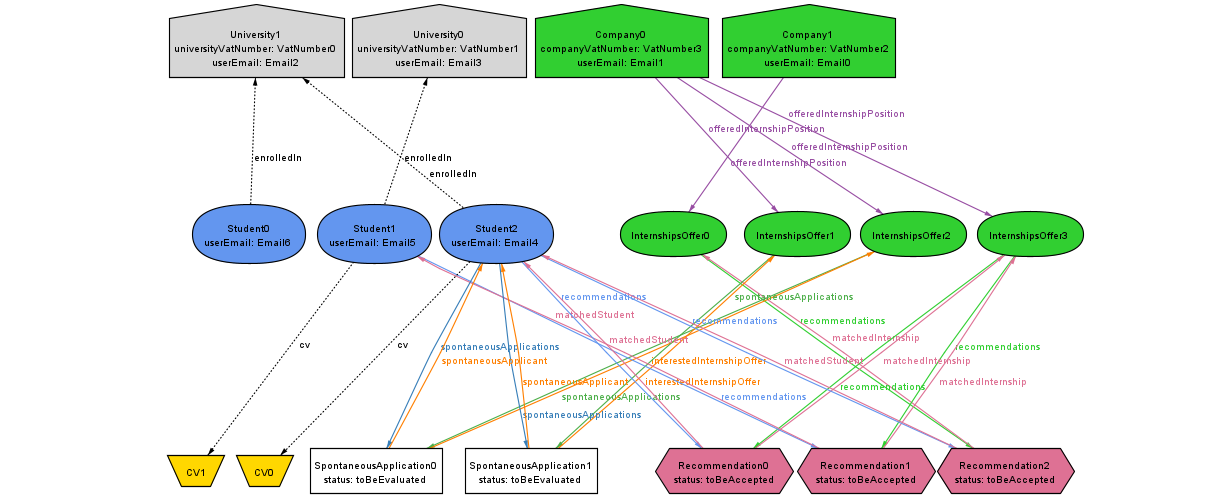
\includegraphics[width=1.3\linewidth]{Alloy/AlloyImage/0.png}
    \caption{Step 0: All Recommendations and Spontaneous Applications have been sent but have not yet been evaluated.}
    \label{fig:ALIMG0}
\end{figure}
\begin{figure}[H]
    \hspace{-2.5cm}
    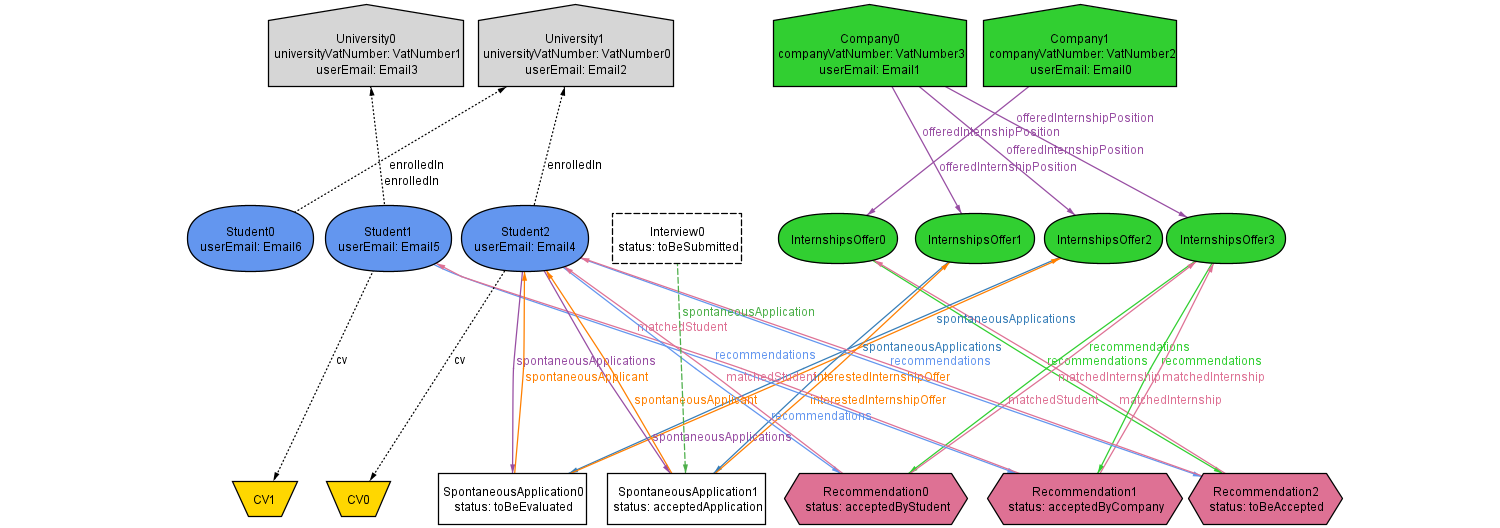
\includegraphics[width=1.3\linewidth]{Alloy/AlloyImage/1.png}
    \caption{Step 1: A Spontaneous Application has been accepted, and an Interview has been created}
    \label{fig:ALIMG1}
\end{figure}
\begin{figure}[H]
    \hspace{-2.5cm}
    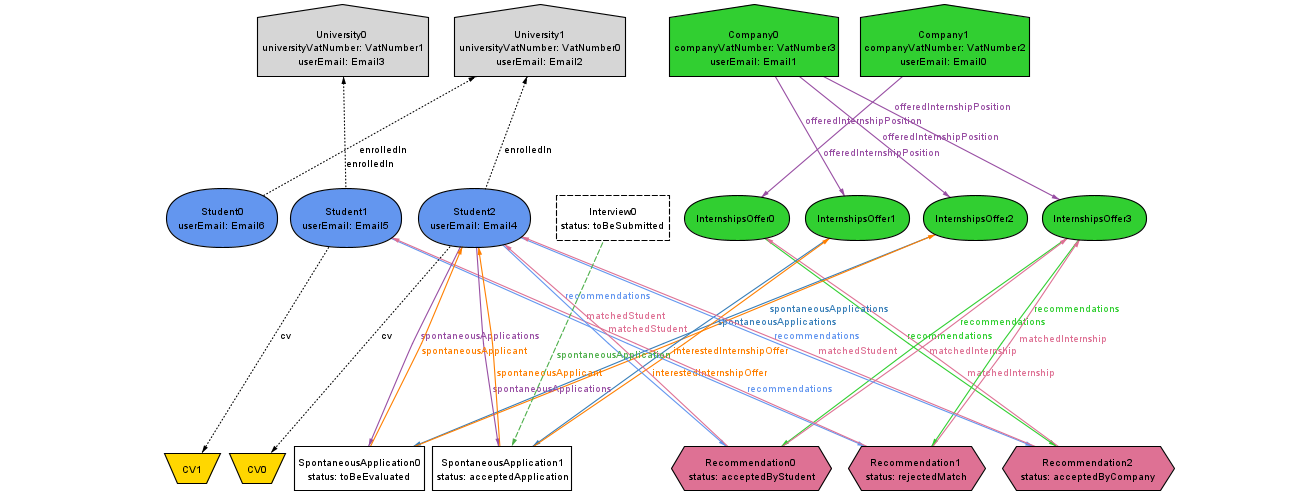
\includegraphics[width=1.3\linewidth]{Alloy/AlloyImage/2.png}
    \caption{Step 2: A Recommendation has been rejected by one of the party}
    \label{fig:ALIMG2}
\end{figure}
\begin{figure}[H]
    \hspace{-2.5cm}
    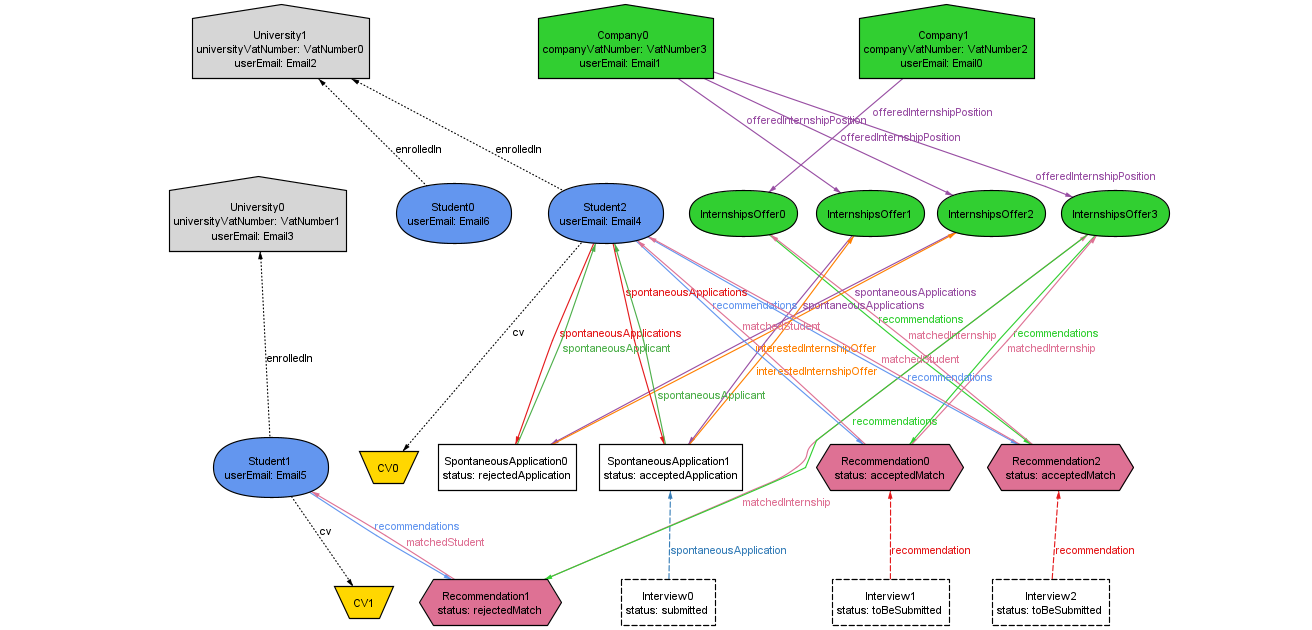
\includegraphics[width=1.3\linewidth]{Alloy/AlloyImage/3.png}
    \caption{Step 3: Another Spontaneous Application has been accepted, and the first Interview has been sent. }
    \label{fig:ALIMG3}
\end{figure}


    %------------------------------------------------------------------------------------------------------------------------------------------------
    \clearpage
    \section{Effort Spent}
    \label{sect:effort}
    \subsection*{Lorenzo Ricci}
\begin{table}[H]
    \centering
\begin{tabular}{|l|c|}
        \hline
        \textbf{Section} & \textbf{Hours} \\ \hline
        Introduction & 10 \\ \hline
        Overall Description & 8 \\ \hline
        Specific Requirements & 15\\ \hline
        Formal Analysis Using Alloy & 10 \\ \hline
        Misc Activities & 20 \\ \hline
    \end{tabular}
    \caption{Effort - Lorenzo Ricci}
    \label{tab:effotricci}
\end{table}
\subsection*{Matteo Giovanni Paoli}
\begin{table}[H]
    \centering
\begin{tabular}{|l|c|}
        \hline
        \textbf{Section} & \textbf{Hours} \\ \hline
        Introduction & 7 \\ \hline
        Overall Description & 16 \\ \hline
        Specific Requirements & 22\\ \hline
        Formal Analysis Using Alloy & 13 \\ \hline
        Misc Activities & 2 \\ \hline
    \end{tabular}
    \caption{Effort - Matteo Giovanni Paoli}
    \label{tab:effotpaoli}
\end{table}
\subsection*{Samuele Grisoni}
\begin{table}[H]
    \centering
\begin{tabular}{|l|c|}
        \hline
        \textbf{Section} & \textbf{Hours} \\ \hline
        Introduction & 11\\ \hline
        Overall Description & 15\\ \hline
        Specific Requirements & 9\\ \hline
        Formal Analysis Using Alloy & 16 \\ \hline
        Misc Activities & 7\\ \hline
    \end{tabular}
    \caption{Effort - Samuele Grisoni}
    \label{tab:effotgrisoni}
\end{table}
    %------------------------------------------------------------------------------------------------------------------------------------------------
    \clearpage
    \addcontentsline{toc}{section}{References}
    \bibliographystyle{plain}
    \bibliography{main}
    %------------------------------------------------------------------------------------------------------------------------------------------------
    
\end{document}
